\documentclass[12pt, twoside, openright]{report} %fuente a 12pt, formato doble pagina y chapter a la derecha
\raggedbottom % No ajustar el contenido con un salto de pagina

% MÁRGENES: 2,5 cm sup. e inf.; 3 cm izdo. y dcho.
\usepackage[
a4paper,
vmargin=2.5cm,
hmargin=3cm
]{geometry}

% INTERLINEADO: Estrecho (6 ptos./interlineado 1,15) o Moderado (6 ptos./interlineado 1,5)
\renewcommand{\baselinestretch}{1.15}
\parskip=6pt

% DEFINICIÓN DE COLORES para portada y listados de código
\usepackage[table]{xcolor}
\definecolor{azulUC3M}{RGB}{0,0,102}
\definecolor{gray97}{gray}{.97}
\definecolor{gray75}{gray}{.75}
\definecolor{gray45}{gray}{.45}

% Soporte para GENERAR PDF/A
\usepackage[a-1b]{pdfx}

% ENLACES
\usepackage{hyperref}
\hypersetup{colorlinks=true,
	linkcolor=black, % enlaces a partes del documento (p.e. índice) en color negro
	urlcolor=blue} % enlaces a recursos fuera del documento en azul

% Añadir pdfs como partes del documento
\usepackage{pdfpages}

% Quitar la indentación de principio de los parrafos
\setlength{\parindent}{0em}

% EXPRESIONES MATEMATICAS
\usepackage{amsmath,amssymb,amsfonts,amsthm}

\usepackage{txfonts} 
\usepackage[T1]{fontenc}
\usepackage[utf8]{inputenc}

% Insertar graficas y fotos
\usepackage{tikz}
\usepackage{pgfplots}

\usepackage[spanish, es-tabla]{babel} 
\usepackage[babel, spanish=spanish]{csquotes}
\AtBeginEnvironment{quote}{\small}

% diseño de PIE DE PÁGINA
\usepackage{fancyhdr}
\pagestyle{fancy}
\fancyhf{}
\renewcommand{\headrulewidth}{0pt}
\fancyfoot[LO,RE]{\thepage}
\fancypagestyle{plain}{\pagestyle{fancy}}

% DISEÑO DE LOS TÍTULOS de las partes del trabajo (capítulos y epígrafes o subcapítulos)
\usepackage{titlesec}
\usepackage{titletoc}
\titleformat{\chapter}[block]
{\large\bfseries\filcenter}
{\thechapter.}
{5pt}
{\MakeUppercase}
{}
\titlespacing{\chapter}{0pt}{0pt}{*3}
\titlecontents{chapter}
[0pt]                                               
{}
{\contentsmargin{0pt}\thecontentslabel.\enspace\uppercase}
{\contentsmargin{0pt}\uppercase}                        
{\titlerule*[.7pc]{.}\contentspage}                 

\titleformat{\section}
{\bfseries}
{\thesection.}
{5pt}
{}
\titlecontents{section}
[5pt]                                               
{}
{\contentsmargin{0pt}\thecontentslabel.\enspace}
{\contentsmargin{0pt}}
{\titlerule*[.7pc]{.}\contentspage}

\titleformat{\subsection}
{\normalsize\bfseries}
{\thesubsection.}
{5pt}
{}
\titlecontents{subsection}
[10pt]                                               
{}
{\contentsmargin{0pt}                          
	\thecontentslabel.\enspace}
{\contentsmargin{0pt}}                        
{\titlerule*[.7pc]{.}\contentspage}  


% DISEÑO DE TABLAS.
\usepackage{multirow} % permite combinar celdas 
\usepackage{caption} % para personalizar el título de tablas y figuras
\usepackage{floatrow} % utilizamos este paquete y sus macros \ttabbox y \ffigbox para alinear los nombres de tablas y figuras de acuerdo con el estilo definido. Para su uso ver archivo de ejemplo 
\usepackage{array} % con este paquete podemos definir en la siguiente línea un nuevo tipo de columna para tablas: ancho personalizado y contenido centrado
\newcolumntype{P}[1]{>{\centering\arraybackslash}p{#1}}
\DeclareCaptionFormat{upper}{#1#2\uppercase{#3}\par}

% Diseño de tabla para ingeniería
\captionsetup[table]{
	format=hang,
	name=Tabla,
	justification=centering,
	labelsep=colon,
	width=.75\linewidth,
	labelfont=small,
	font=small,
}

% DISEÑO DE FIGURAS.
\usepackage{graphicx}
\graphicspath{{img/}} %ruta a la carpeta de imágenes

% Diseño de figuras para ingeniería
\captionsetup[figure]{
	format=hang,
	name=Fig.,
	singlelinecheck=off,
	labelsep=colon,
	labelfont=small,
	font=small		
}

% NOTAS A PIE DE PÁGINA
\usepackage{chngcntr} %para numeración continua de las notas al pie
\counterwithout{footnote}{chapter}

% LISTADOS DE CÓDIGO
% soporte y estilo para listados de código. Más información en https://es.wikibooks.org/wiki/Manual_de_LaTeX/Listados_de_código/Listados_con_listings
\usepackage{listings}

% definimos un estilo de listings
\lstdefinestyle{estilo}{ frame=Ltb,
	framerule=0pt,
	aboveskip=0.5cm,
	framextopmargin=3pt,
	framexbottommargin=3pt,
	framexleftmargin=0.4cm,
	framesep=0pt,
	rulesep=.4pt,
	backgroundcolor=\color{gray97},
	rulesepcolor=\color{black},
	%
	basicstyle=\ttfamily\footnotesize,
	keywordstyle=\bfseries,
	stringstyle=\ttfamily,
	showstringspaces = false,
	commentstyle=\color{gray45},     
	%
	numbers=left,
	numbersep=15pt,
	numberstyle=\tiny,
	numberfirstline = false,
	breaklines=true,
	xleftmargin=\parindent
}

\captionsetup[lstlisting]{font=small, labelsep=period}
% fijamos el estilo a utilizar 
\lstset{style=estilo}
\renewcommand{\lstlistingname}{\uppercase{Código}}

\pgfplotsset{compat=1.17} 
%-------------
%	DOCUMENTO
%-------------

\begin{document}
\pagenumbering{roman} % Se utilizan cifras romanas en la numeración de las páginas previas al cuerpo del trabajo
	
%----------
%	PORTADA
%----------	
\begin{titlepage}
	\begin{sffamily}
	\color{azulUC3M}
	\begin{center}
		\begin{figure}[H] %incluimos el logotipo de la Universidad
			\makebox[\textwidth][c]{
\includegraphics[width=16cm]{Portada_Logo.png}}
		\end{figure}
		\vspace{2.5cm}
		\begin{Large}
			Grado en Ingeniería Informática\\			
			2020-2021\\
			\vspace{2cm}		
			\textsl{Apuntes}\\
			\bigskip
		\end{Large}
		 	{\Huge Aprendizaje Automático}\\
		 	\vspace*{0.5cm}
	 		\rule{10.5cm}{0.1mm}\\
			\vspace*{0.9cm}
			{\LARGE Jorge Rodríguez Fraile\footnote{\href{mailto:100405951@alumnos.uc3m.es}{Universidad: 100405951@alumnos.uc3m.es}  |  \href{mailto:jrf1616@gmail.com}{Personal: jrf1616@gmail.com}}}\\ 
			\vspace*{1cm}
	\end{center}
	\vfill
	\color{black}
		
\includegraphics[width=4.2cm]{img/creativecommons.png}\\
		Esta obra se encuentra sujeta a la licencia Creative Commons\\ \textbf{Reconocimiento - No Comercial - Sin Obra Derivada}
	\end{sffamily}
\end{titlepage}

%----------
%	ÍNDICES
%----------	

%--
% Índice general
%-
\tableofcontents
\thispagestyle{fancy}

%--
% Índice de figuras. Si no se incluyen, comenta las líneas siguientes
%-
\listoffigures
\thispagestyle{fancy}

%----------
%	TRABAJO
%----------	
\pagenumbering{arabic} % numeración con números arábigos para el resto de la publicación	


%----------
%	COMENZAR A ESCRIBIR AQUI
%----------	
\chapter{Información}
\section{Profesores}

\begin{quote}
Teorías: Raquel Fuentetaja rfuentet@inf.uc3m.es 2.1B19

Prácticas: Rubén Majadas rmajadas@pa.uc3m.es 2.2A12
\end{quote}

\section{Presentación}

Vamos a trabajar sobre una modificación del Pac-man.

Los fantasmas no van a por Pac-man, sino que si los toca se los come.

Las prácticas consisten en 4 Tutoriales 0.5 cada uno y 2 Prácticas 1.5 cada una.

El objetivo de la asignatura es conseguir que gane solo el Pac-man sin ayuda nuestra.

El objetivo de las prácticas no es pegar los resultados o con captura, sino documentar bien, incluyendo tablas y gráficas.

Los casos que no funcionan son importantes, no solo poner pruebas con éxito. Así se documentan los cambios realizados.


\chapter{Tema 1: Introducción}

\textbf{Definición}:

Campo de estudio que da al computador la habilidad de aprender.

Un programa se dice que aprende de una experiencia con respecto a una tarea y alguna medida del rendimiento, si el rendimiento con la tarea al ser medido mejora con la experiencia.

\textbf{Objetivo}: Aprender conocimiento nuevo y mejorar el comportamiento de un sistema.

Se encuentra en las fronteras de la programación.

\textbf{Programación tradicional}: Lo normal, es que el usuario construya el programa que resuelve el problema.

\begin{figure}[H]
	\ffigbox[\FBwidth]
	{\caption{Programación tradicional}}
	{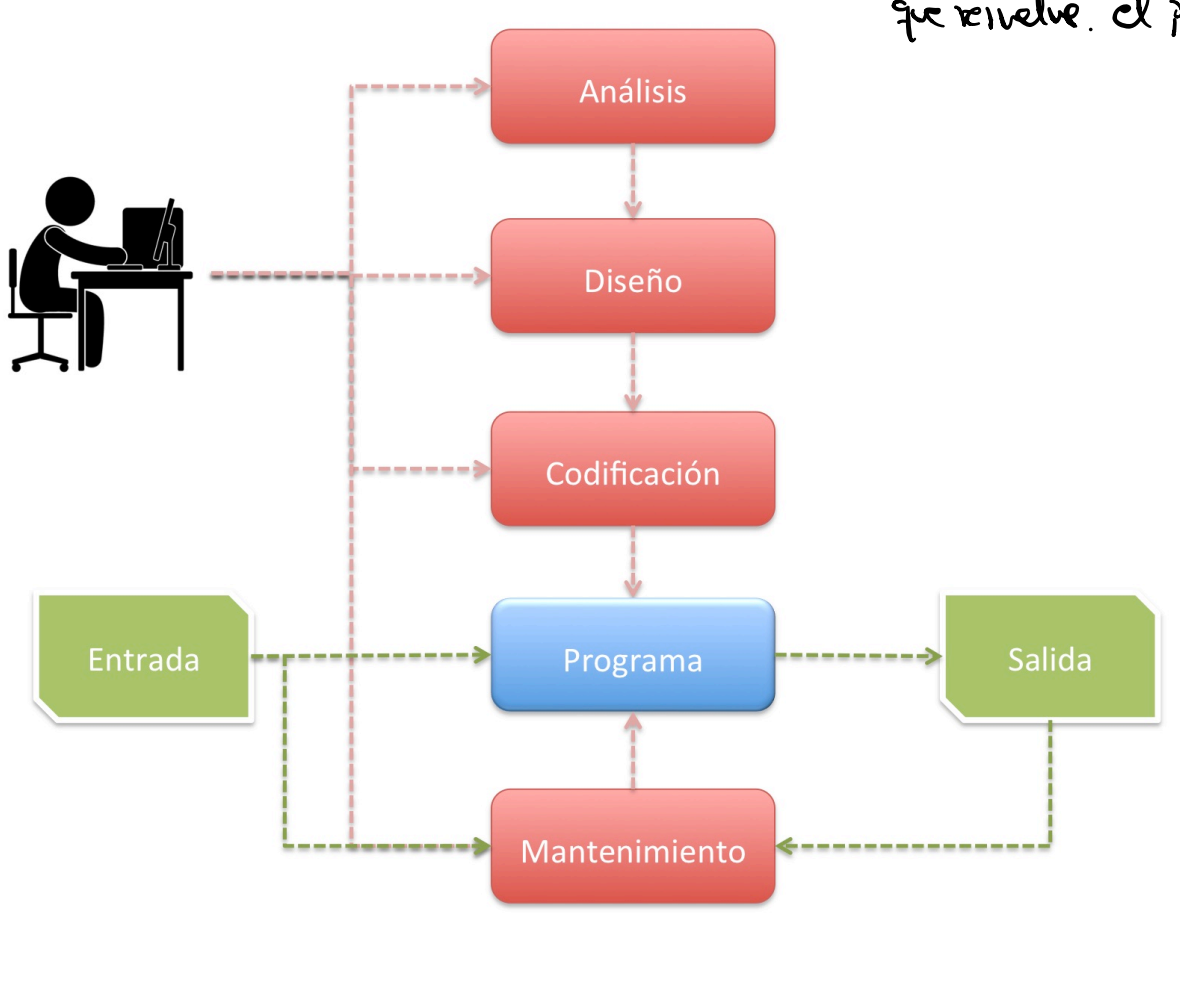
\includegraphics[scale=.15]{Untitled.png}}
\end{figure}

\textbf{Programación automática}: Se crea un programa capaz de generar
el programa que es capaz de resolver nuestro problema.

\begin{figure}[H]
	\ffigbox[\FBwidth]
	{\caption{Programación automática}}
	{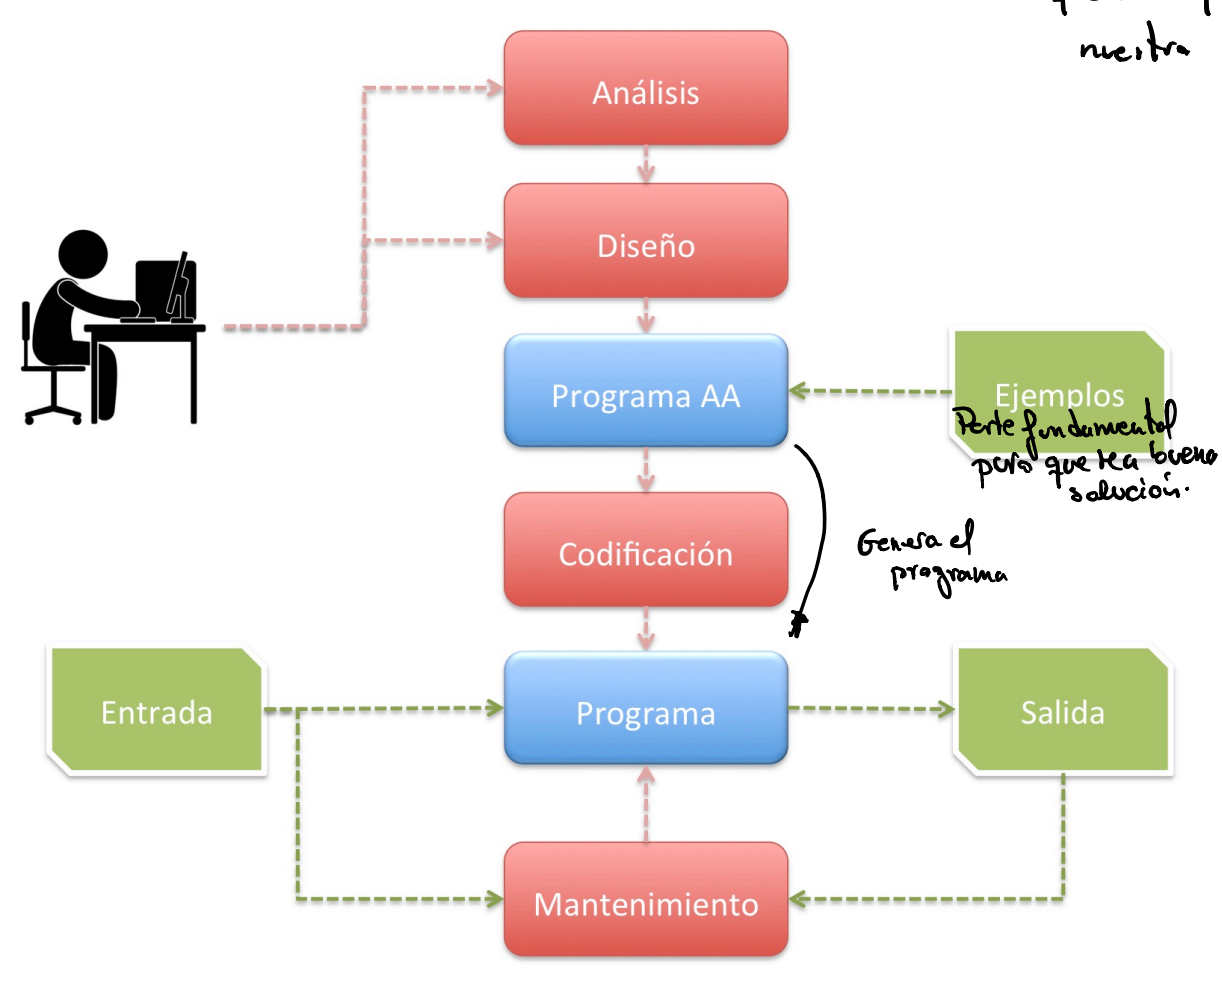
\includegraphics[scale=.15]{Untitled 1.png}}
\end{figure}

\pagebreak

\textbf{Es útil cuando:}

\begin{itemize}
\item
  No existe experiencia humana.
\item
  Los humanos no saben explicar su experiencia.
\item
  Los modelos deben ser personalizados
\item
  Los modelos se basan en enormes cantidades de datos.
\end{itemize}

\textbf{Actualmente}: Existen muchos algoritmos de aprendizaje
automático efectivo y eficientes, recursos computacionales y datos
disponibles.

\textbf{Definición de tarea de Aprendizaje Automático}: Mejorar en una
\textbf{tarea} T, respecto a una \textbf{medida de rendimiento} P,
basándose en la \textbf{experiencia} E (los ejemplos).

Tarea, Medida y Experiencia.

\begin{figure}[H]
	\ffigbox[\FBwidth]
	{\caption{Tipos de tareas de Aprendizaje Automático}}
	{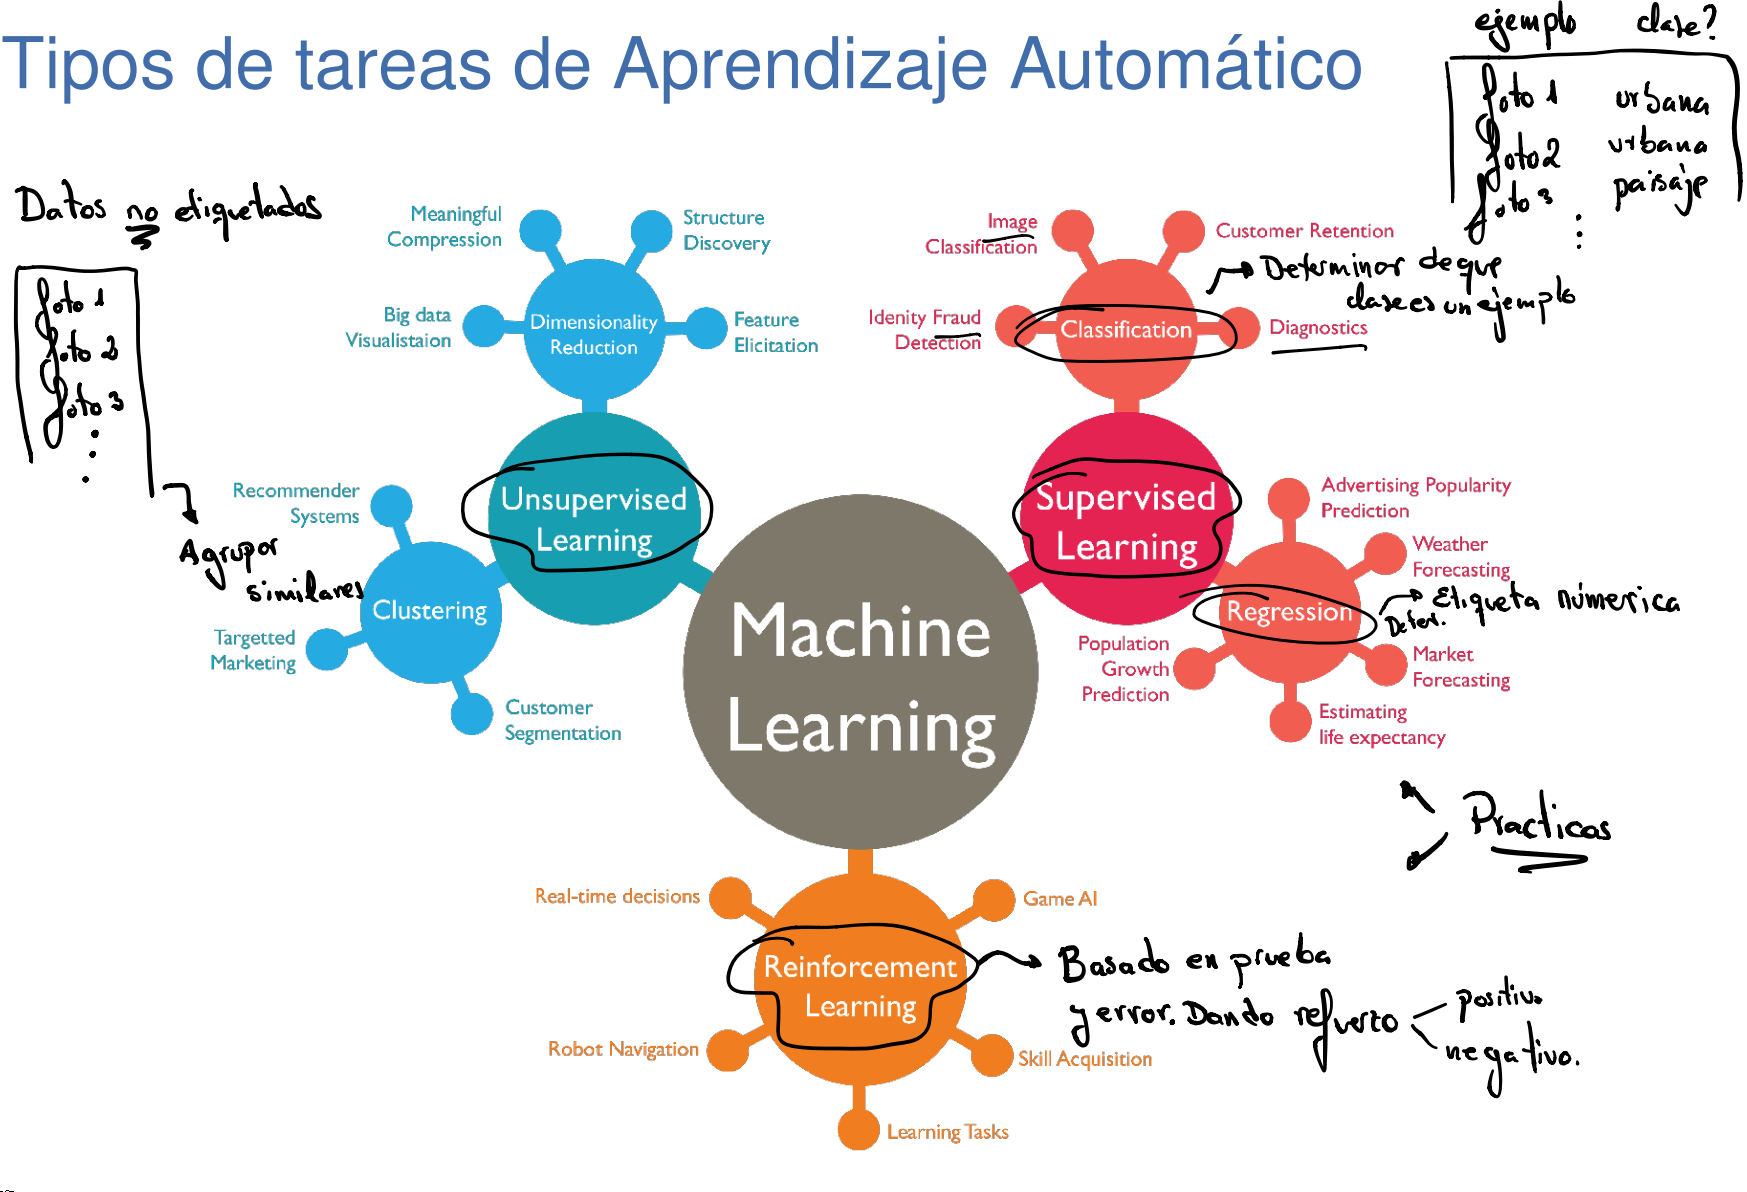
\includegraphics[scale=.2]{Untitled 2.png}}
\end{figure}
\pagebreak
\textbf{Tipos de tareas de Aprendizaje Automático:}
\begin{itemize}

\item
  \textbf{Aprendizaje supervisado}: Consiste en etiquetar los datos.

  \begin{itemize}
  
  \item
    \textbf{Clasificación}: Determinar de qué clase es un ejemplo.
    
  \item
    \textbf{Predicción -- Regresión}: Determinar una etiqueta numérica.

  \end{itemize}
\item
  \textbf{Aprendizaje no supervisado}: Agrupa elementos similares, no
  etiqueta.

  \begin{itemize}
  
  \item
    \textbf{Agrupación}.
  \end{itemize}
\item
  \textbf{Aprendizaje por refuerzo}: Basado en prueba y error. Dando
  refuerzo positivo/negativo.
\end{itemize}

\textbf{Algunas aplicaciones}: Sanidad, Domótica, Banca, Marketing,
Personalización, Seguridad, Videojuego, etc.

\textbf{Problemas no técnicos:}

\begin{itemize}
\item
  Las máquinas no son responsables de los diagnósticos, predicciones, o
  clasificaciones que hacen.
\item
  Los humanos no se fían de los resultados.
\item
  La salida no es entendible por el humano. No explica sus decisiones,
  se está avanzando para lograr saber cómo piensa.
\item
  Leyes de protección de datos.
\item
  Miedo de los humanos a la pérdida de control.
\item
  Cuestiones éticas.
\end{itemize}

\chapter{Tema 2: Árboles y Reglas de Decisión}

\section{Aprendizaje inductivo (De lo más específico a lo más general)}

Encontrar una \textbf{función h} (la hipótesis o modelo) que aproxime la \textbf{función f} (desconocida) definida por un conjunto de ejemplos.

Los ejemplos normalmente se representan como pares, \textbf{(x, f(x))}.

\textbf{Según como sea la salida de f}: Es \textbf{clasificación} si es
categórica y es de \textbf{regresión} si es numérica.

Se basa en inducción, se parte de un ejemplo específico para obtener
modelos generales.

\textbf{Asume que:}

\begin{itemize}
\item
  La \textbf{hipótesis del aprendizaje es inductiva.}
\item
  Si un modelo o hipótesis \textbf{categoriza bien en función a un
  conjunto de ejemplos grande también lo hará bien para futuros
  ejemplos.}
\item
  \textbf{Siempre hay un sesgo inductivo}, que influye en la decisión,
  nos lleva más a uno que a otro.
\item
  El lenguaje de representación nos limita si no lo puede expresar bien.
  Por ejemplo, limitarnos a una función lineal, pero es cuadrática.
\item
  Encontrar una hipótesis adecuada puede ser difícil, f es desconocida y
  puede ser complicado determinar si h es buena.
\end{itemize}

El \textbf{espacio de hipótesis} es el conjunto de hipótesis que se consideran para aproximar f, \textbf{influye mucho para encontrar una
buena aproximación}, pueden ser: funciones lineales, polinómicas, lógica de predicados, árboles de decisión, etc.

Los ejemplos tienen atributos/características que los identifican y nos permitirán clasificarlos por clases. Cada ejemplo es una instancia, da valor a los atributos y su clase.

Todos los ejemplos clasificados forman el conjunto de entrenamiento.

\section{Definiciones}

\textbf{Atributos}: Característica que define a un elemento de un conjunto.

\textbf{Instancia}: Colección de valores de atributos.

\textbf{Clase}: Cada uno de los subconjuntos disjuntos.

\textbf{Ejemplo (positivo)}: Instancia que pertenece al subconjunto definido por la clase.

\textbf{Ejemplo negativo}: No pertenece al subconjunto definido por la clase.

\textbf{Generalización de un conjunto de ejemplos de una clase (hipótesis)}: Descripción que representa al subconjunto de instancias de la clase y no de otras.

\section{Árboles y reglas de decisión}

Usaremos \textbf{modelos simbólicos como árboles de decisión}, que usan símbolos para representar lo que los hace más fáciles para ver explicaciones de las decisiones, las podemos entender. Sin embargo, en otros tipos de modelos como los numéricos (redes neuronales), usa números para representar y no es posible que dé explicaciones que entendamos.

\section{Aprendizaje de árboles de
decisión}

Nosotros estudiaremos \textbf{ID3 (Dicotomizador Iterativo, Quinlan 1986)}, a partir de ejemplos de partida genera árboles de decisión. Normalmente NO son árboles binarios.

Usa búsqueda avara, para encontrar el árbol más sencillo que separa mejor los ejemplos. Utiliza una heurística basada en entropía. Trata de escoger para empezar la clasificación el atributo que mejor separa las distintas clases.

\section{Algoritmo}

\begin{enumerate}
\def\labelenumi{\arabic{enumi}.}
\item
  \textbf{Seleccionar el atributo} \(A_i\) que maximice la ganancia
  \(G(A_i)\).
\item
  \textbf{Crear un nodo} para ese atributo con \textbf{tantos sucesores como valores} tenga.
\item
  \textbf{Dividir los ejemplos} en los sucesores según el valor del atributo.
\item
  Por cada sucesor,

  sí solo hay \textbf{ejemplo de una clase}, entonces se \textbf{etiqueta con esa clase},

  si no, \textbf{ejecutar el ID3} con la tabla formada por los ejemplos de ese nodo, pero sin el atributo que todos tiene en común.
\end{enumerate}
\pagebreak
  Ejemplo:
\begin{figure}[H]
	\ffigbox[\FBwidth]
	{\caption{Diagramas ID3 I}}
	{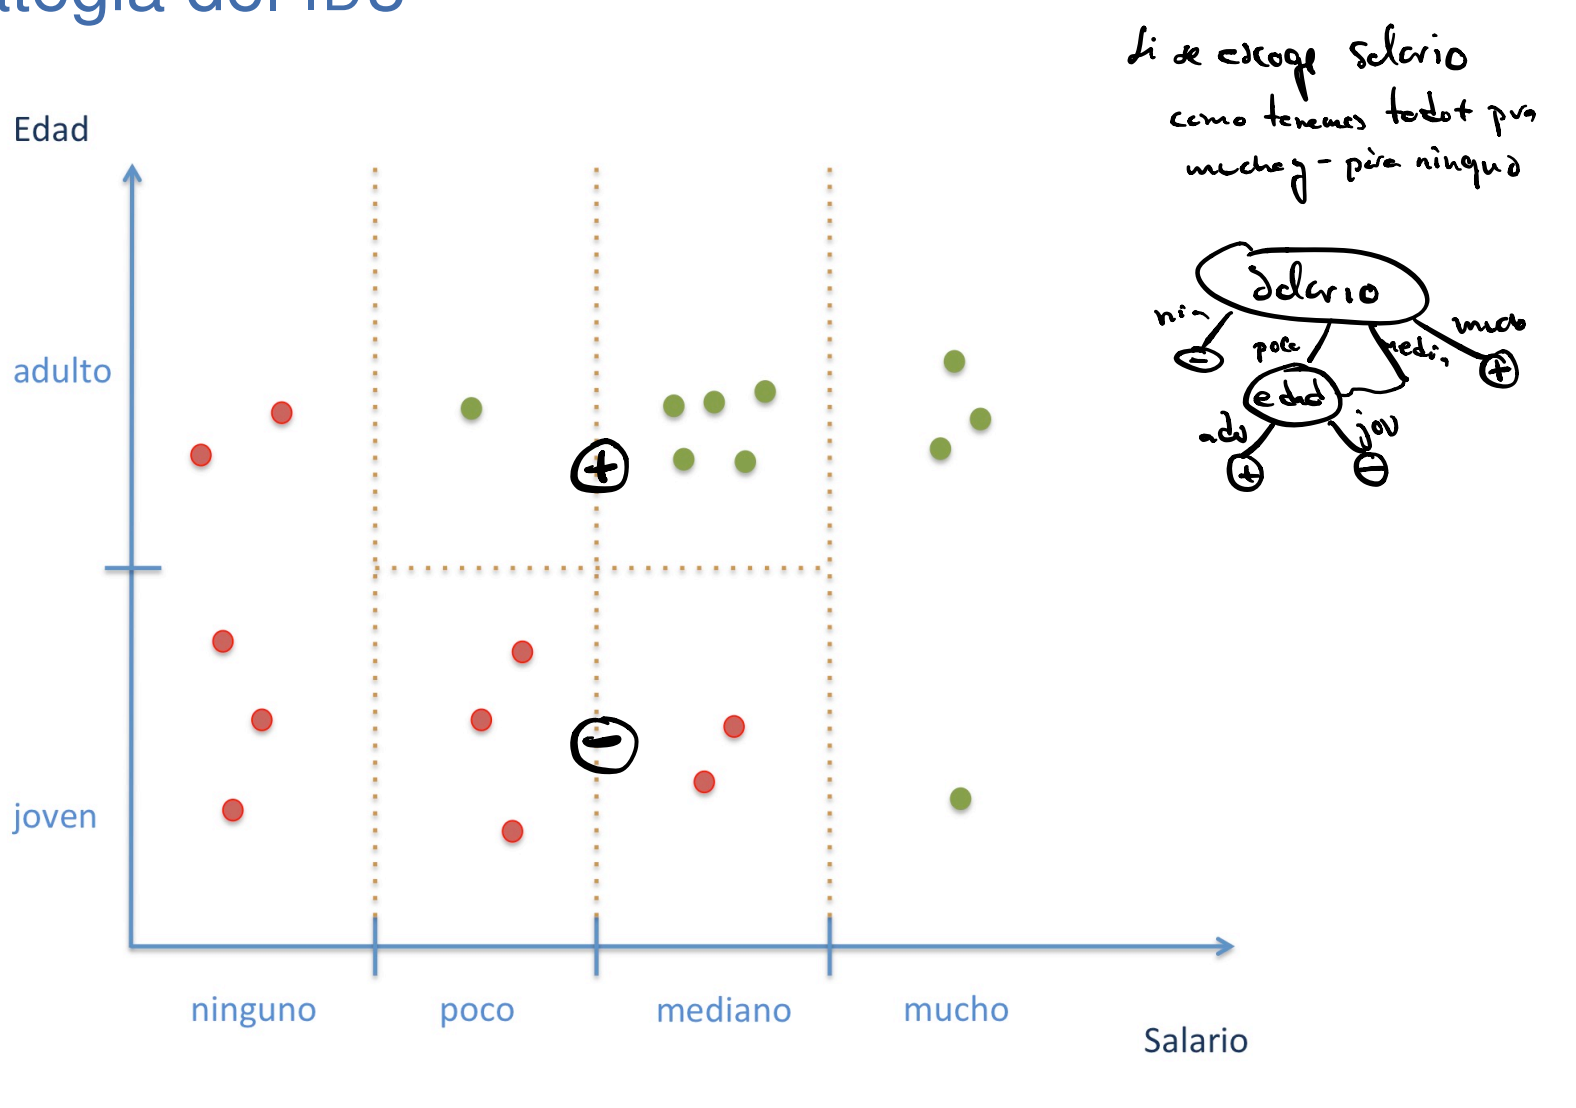
\includegraphics[scale=.2]{Untitled 3.png}}
\end{figure}
\begin{figure}[H]
	\ffigbox[\FBwidth]
	{\caption{Diagramas ID3 II}}
	{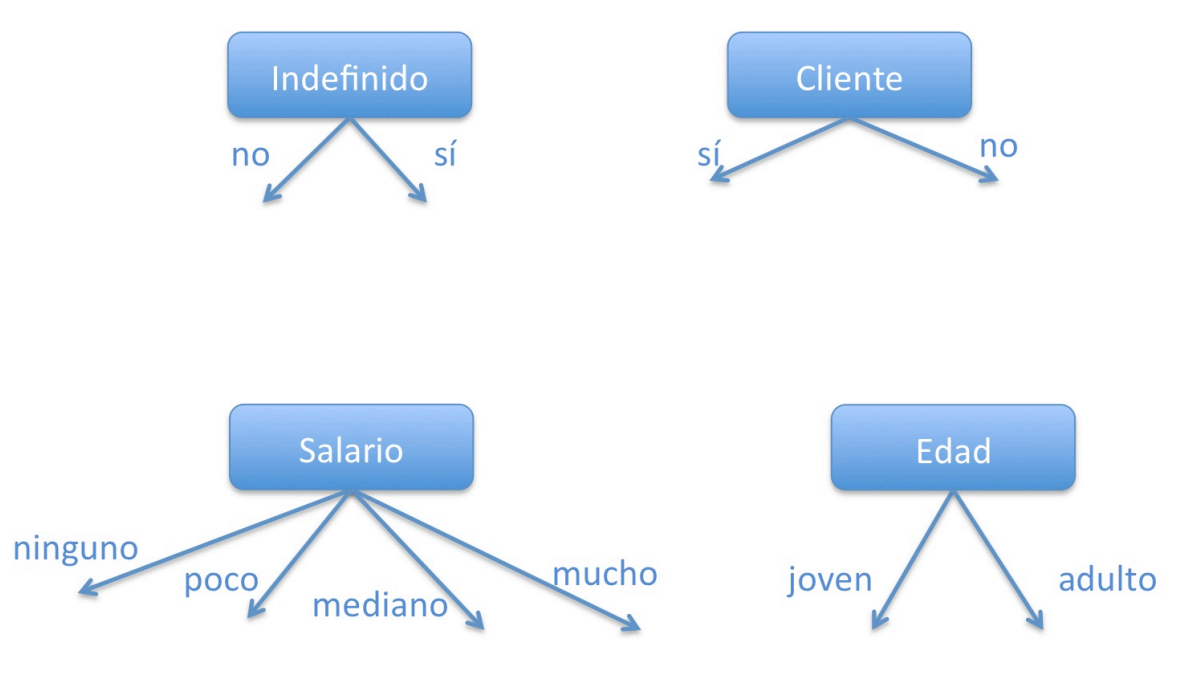
\includegraphics[scale=.2]{Untitled 4.png}}

\end{figure}
\begin{figure}[H]
	\ffigbox[\FBwidth]
	{\caption{Diagramas ID3 III}}
	{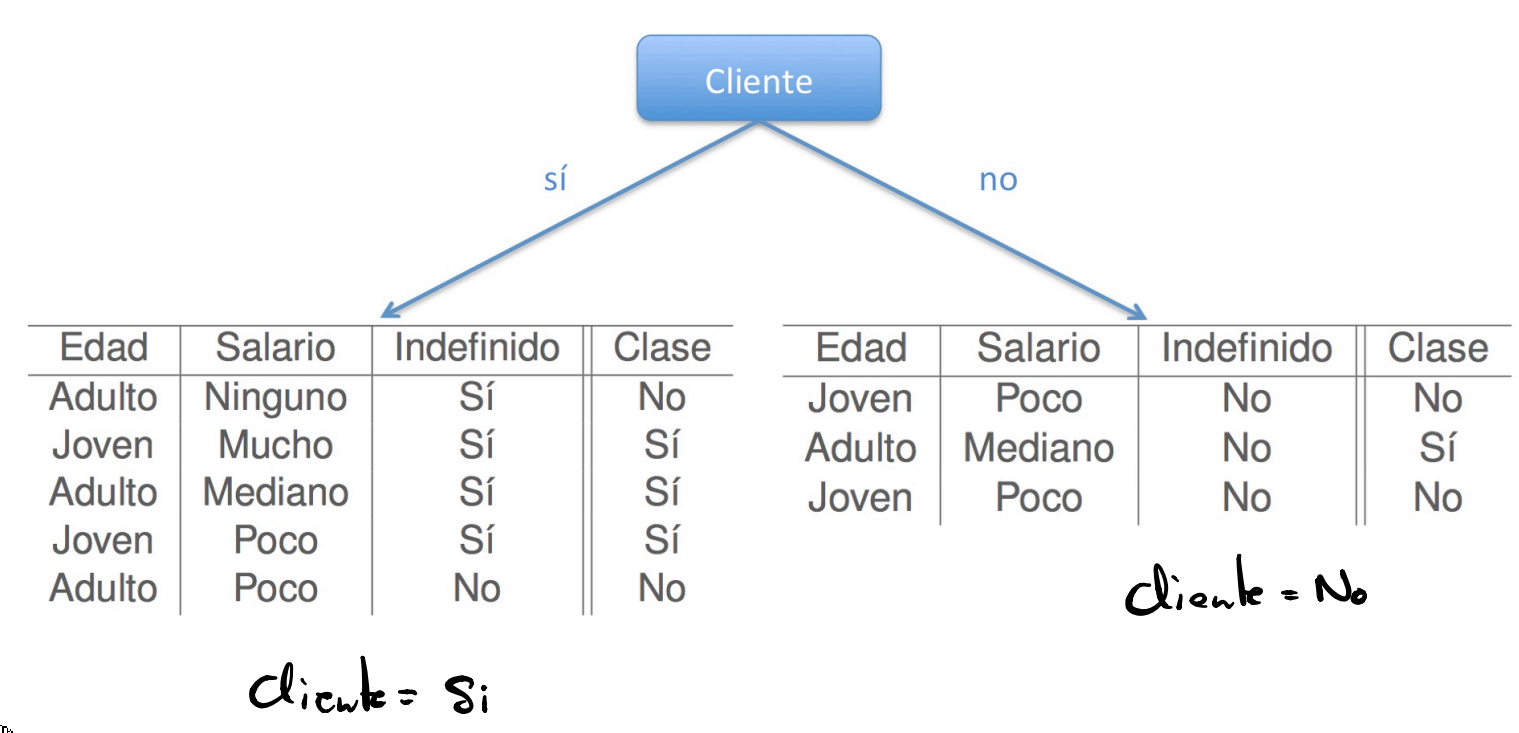
\includegraphics[scale=.2]{Untitled 5.png}}
\end{figure}
\begin{figure}[H]
	\ffigbox[\FBwidth]
	{\caption{Diagramas ID3 IV}}
	{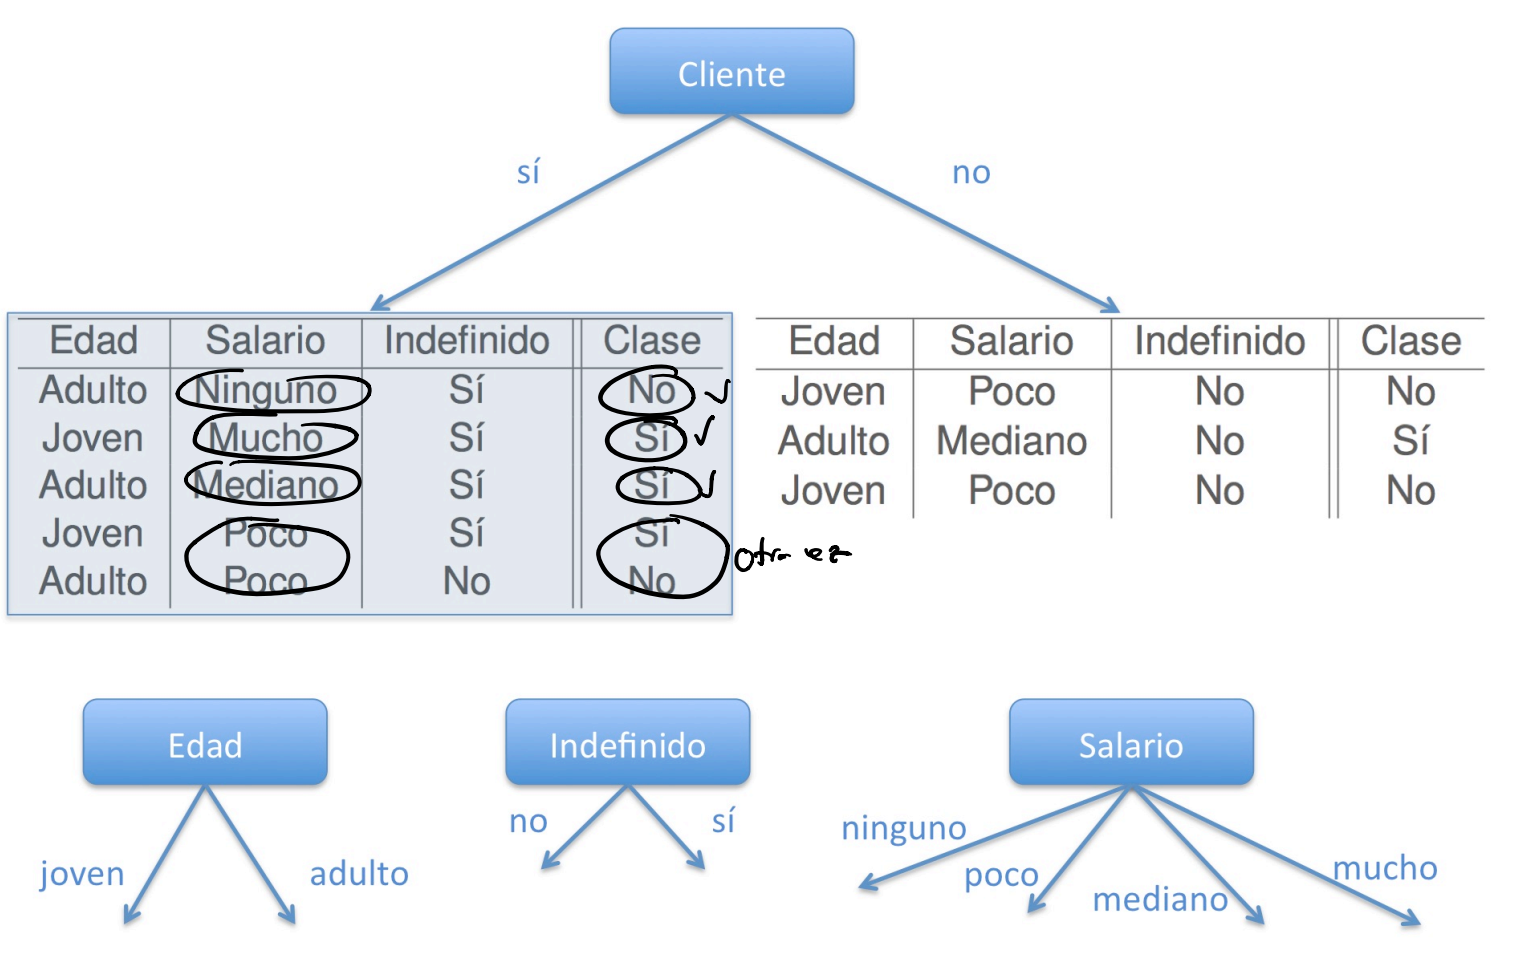
\includegraphics[scale=.2]{Untitled 6.png}}
\end{figure}
\begin{figure}[H]
	\ffigbox[\FBwidth]
	{\caption{Diagramas ID3 V}}
	{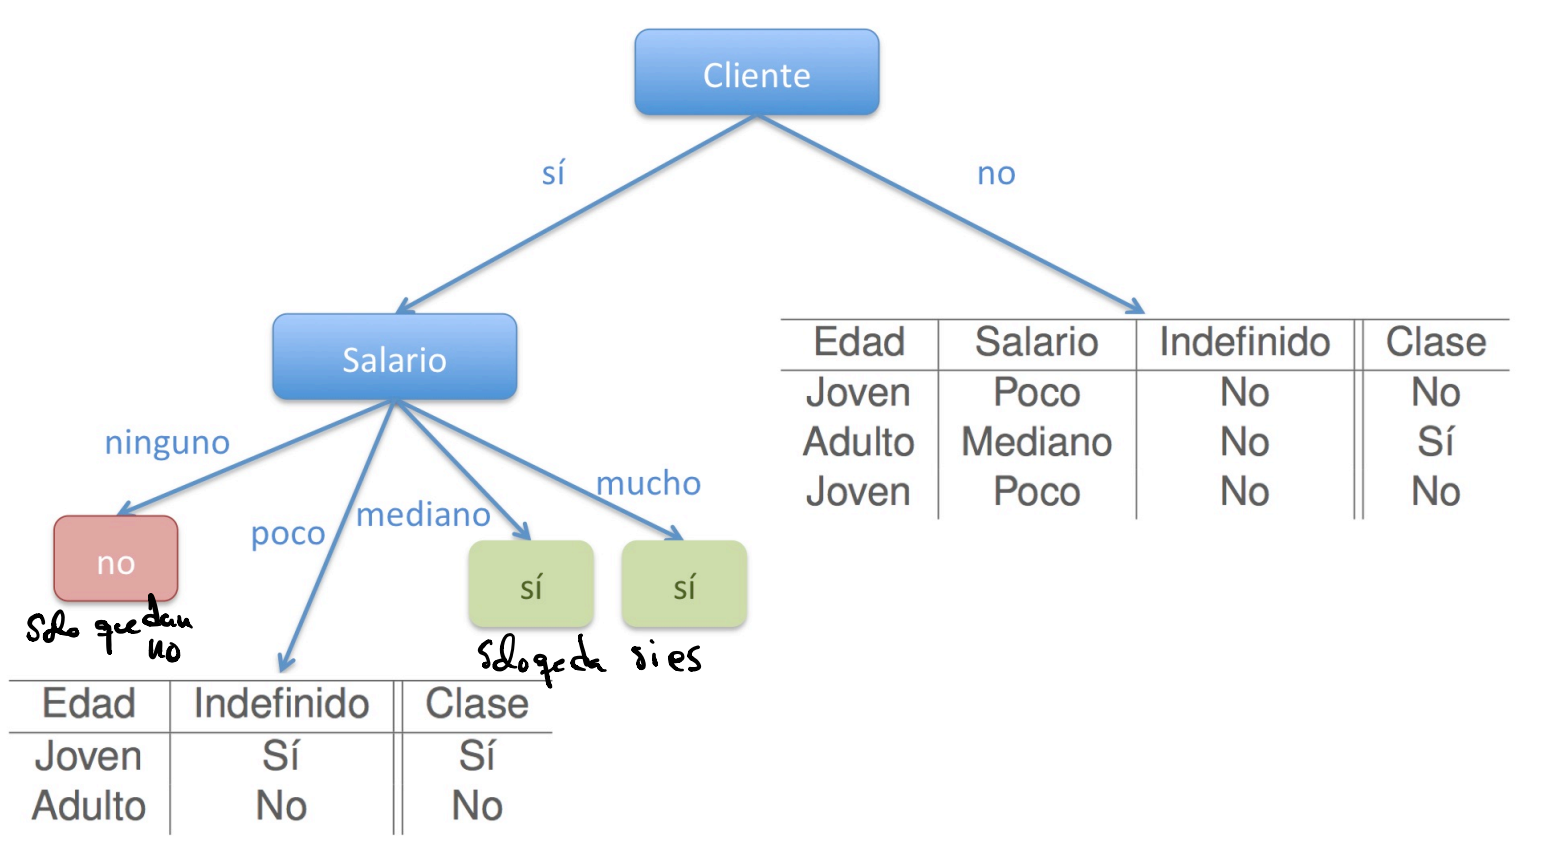
\includegraphics[scale=.2]{Untitled 7.png}}
\end{figure}
\begin{figure}[H]
	\ffigbox[\FBwidth]
	{\caption{Diagramas ID3 VI}}
	{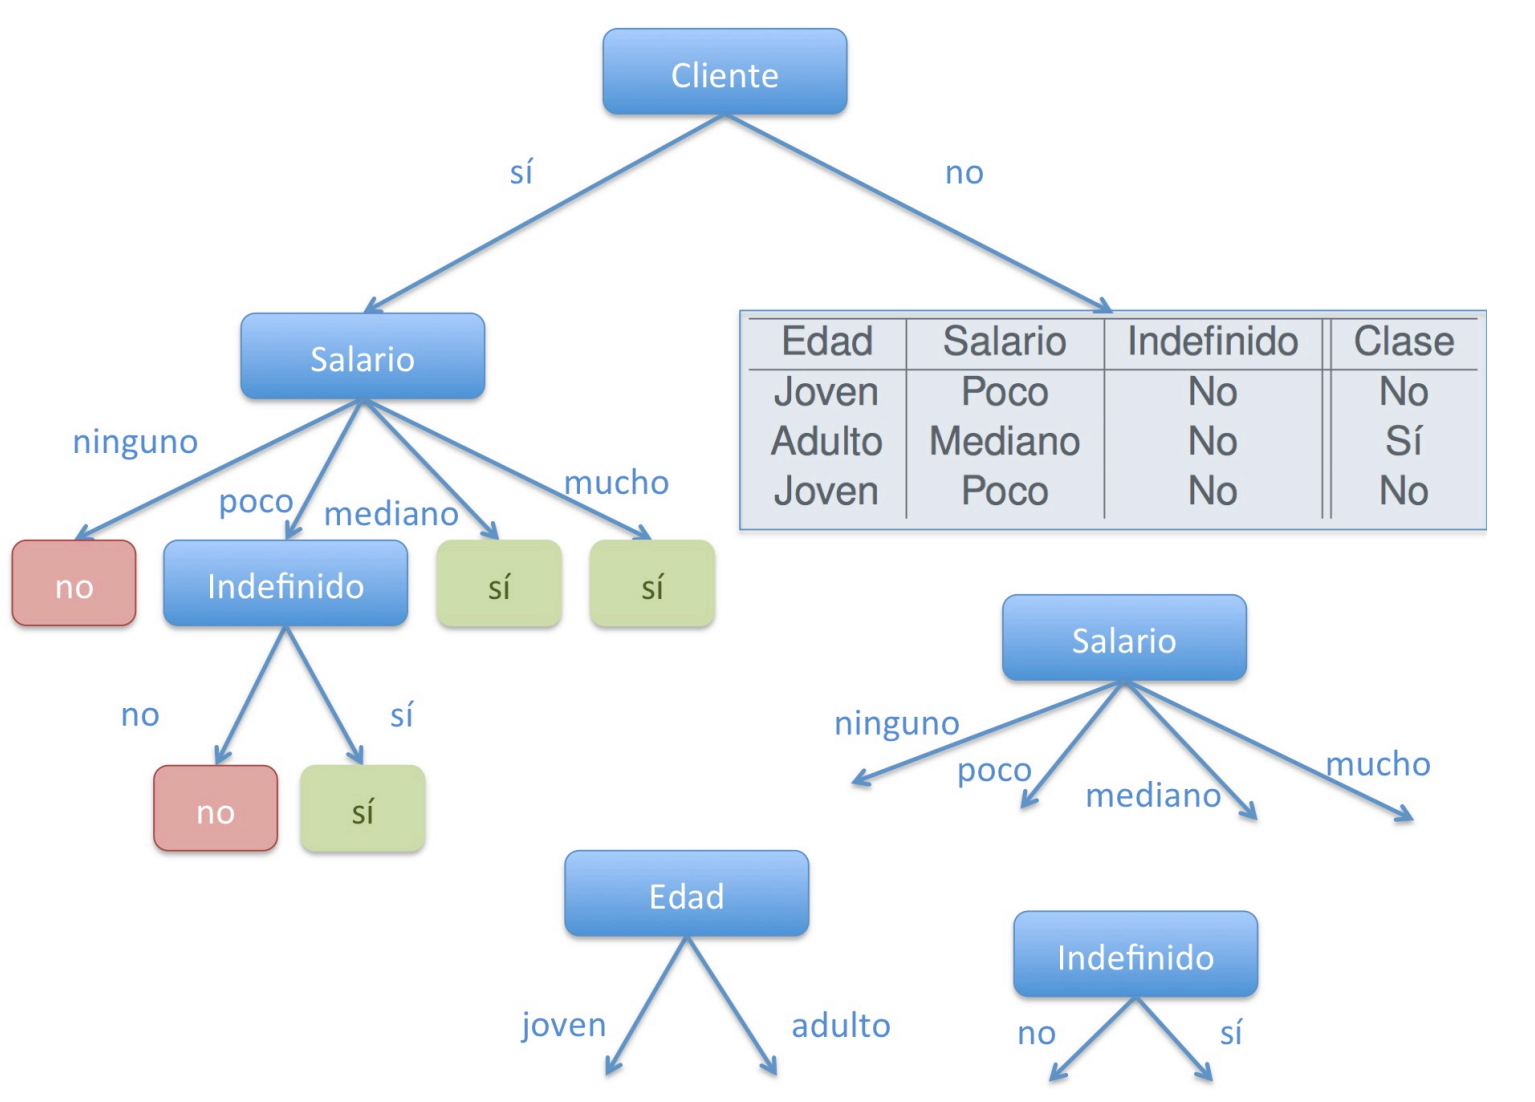
\includegraphics[scale=.2]{Untitled 8.png}}
\end{figure}
\begin{figure}[H]
	\ffigbox[\FBwidth]
	{\caption{Diagramas ID3 VII}}
	{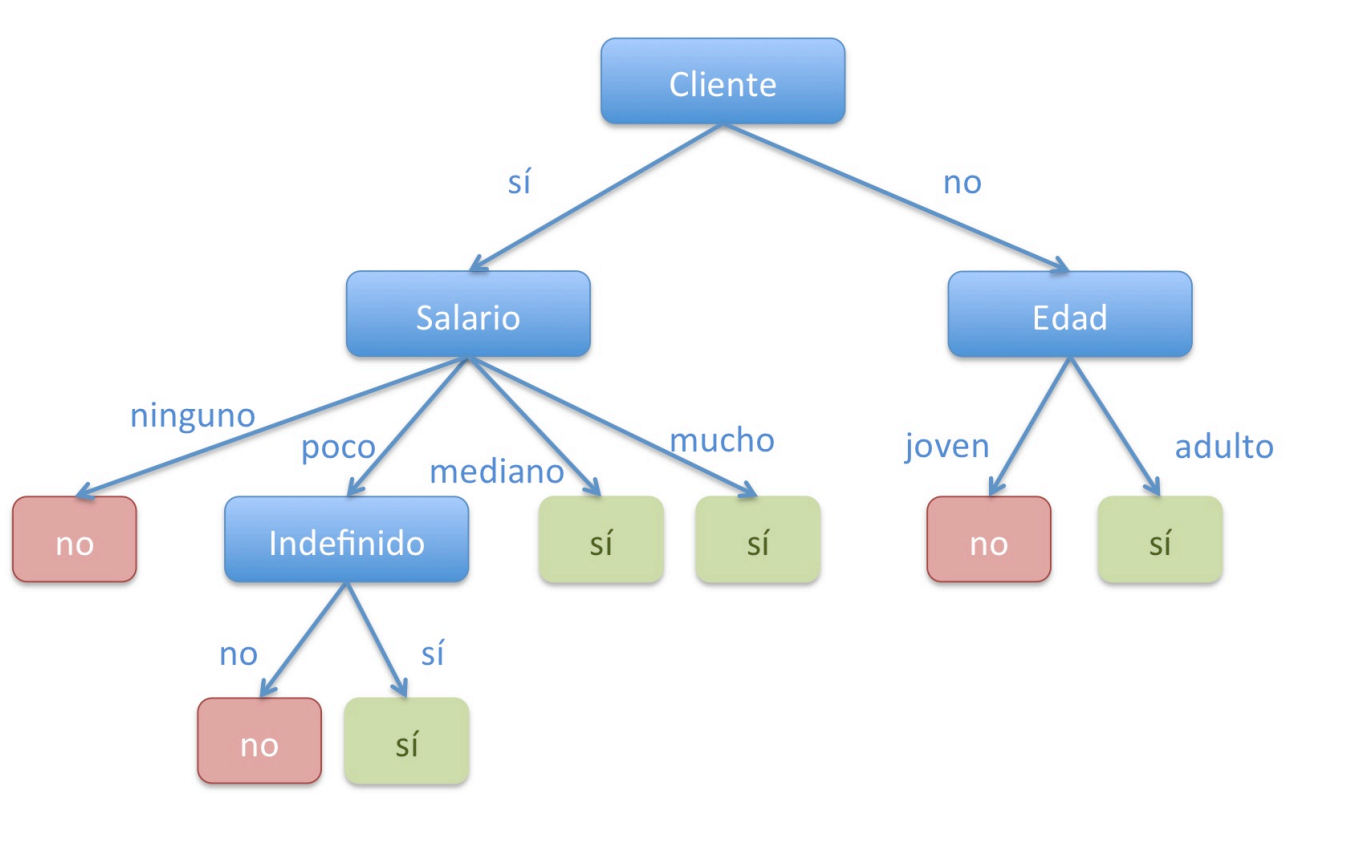
\includegraphics[scale=.2]{Untitled 9.png}}
\end{figure}


\section{Heurística de ID3 (Heurística de la ganancia de
información)}

Seleccionar el \textbf{atributo que mejor separe los ejemplos de acuerdo
con las clases}, que deje subconjuntos más puros (orientados más a un
valor)

Para calcular la ganancia se utiliza el concepto de Entropía, como medida de la pureza o impureza de un conjunto ejemplos.
\pagebreak
\section{Entropía}

\textbf{Entropía en clasificación binaria}: El conjunto de ejemplos S
pertenece a una de las dos clases:
\textbf{\(Entropia(S) \equiv -p_\oplus \log _2 p_\oplus -p_\ominus \log _2 p_\ominus\)}

\begin{itemize}
\item
  \(p_\oplus\): \textbf{Proporción} de ejemplos \textbf{positivos} sobre el total.
\item
  \(p_\ominus\): \textbf{Proporción} de ejemplos \textbf{negativos} sobre el total.
\end{itemize}

\(p_\oplus+p_\ominus=1\)

\(p_\oplus+p_\ominus=0.5\) Entropía máxima

\textbf{Entropía en múltiples clases}:
\(Entropia(S) \equiv \sum_{c\in C} -p_c \log _2 p_c\)

Cuanto más se diferencian las proporciones, cuanto más notablemente hay de una que de otra, más tiende a 0.

\textbf{Nuestro objetivo es minimizar la entropía.}

\textbf{La ganancia de información:} mide la efectividad de un atributo
para clasificar, es la \textbf{reducción esperada de la entropía} cuando
se divide el conjunto de datos original S según el atributo dado A.
\begin{figure}[H]
  \begin{itemize}
    \item
      \(G(S, A)=Entropia(S) - Entropia\_ Atr(S, A)\)
    \item
      \(Entropia\_ Atr(S, A)= \sum_{c \in valores(A)} \frac {|S_{A=v}|}{|S|} Entropia(S_{A=v})\)
    \item
      \(Entropia(S_{A=v})= -\sum_{c \in C} \frac {|S_{A=v, C=c}|}{|_{A=v}|} \log_2 \frac {|S_{A=v,C=c}|}{|_{A=v}|}\)
    \end{itemize}
    \captionsetup{justification=centering}
  \caption{Fórmulas Entropía}
\end{figure}


\textbf{Se elige el atributo que maximiza la ganancia de información},
ya que menos resta es el que menos entropía tiene, o elegir el que menor
\textbf{entropía tenga}.

\(A= \arg\max_{A \in \mathcal{A}} G(S,A) = \arg\min_{A \in \mathcal{A}} Entropia \_ Atr(A,S)\)


\begin{figure}[H]
	Ejemplo
	\ffigbox[\FBwidth]
	{\caption{Ejemplo cálculo de entropía}}
	{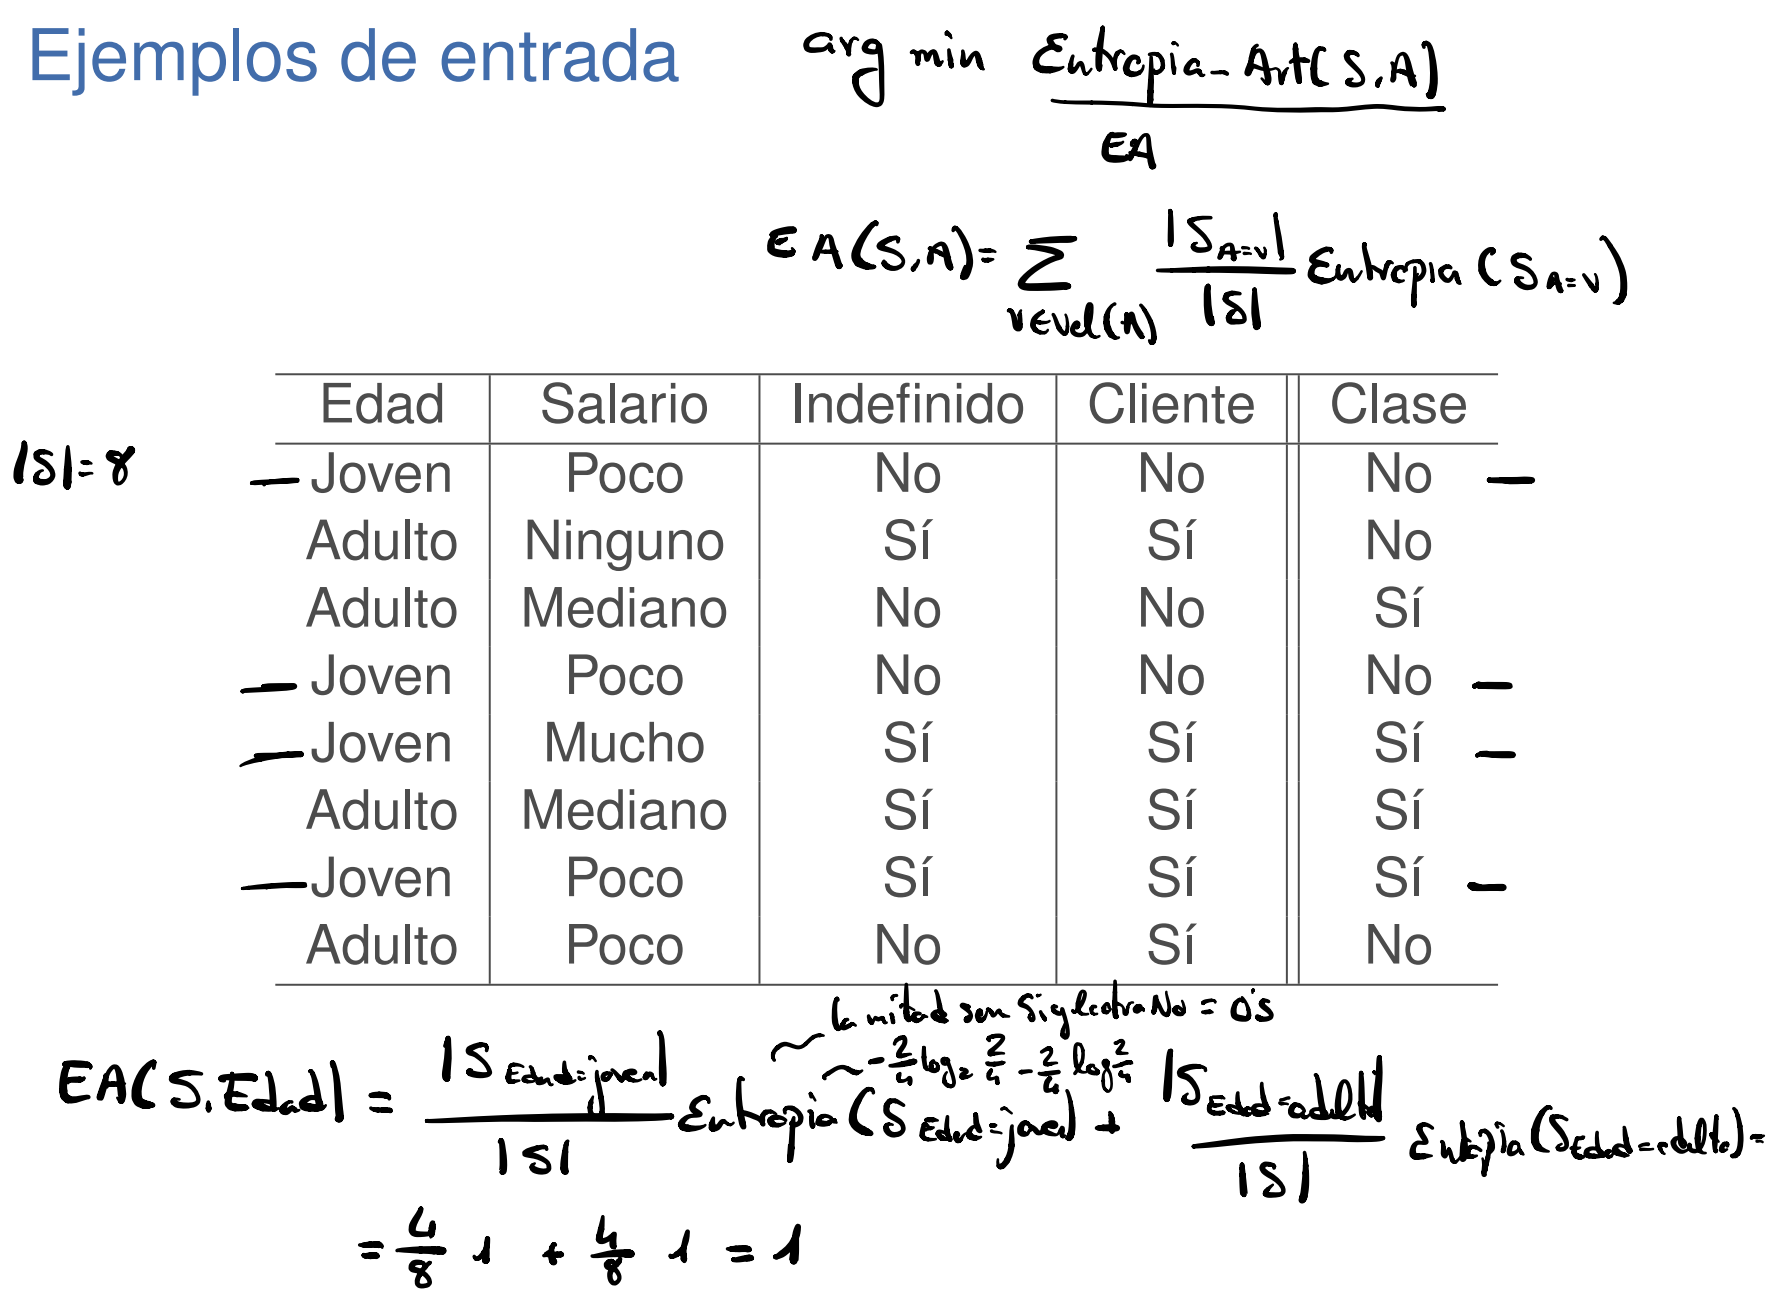
\includegraphics[scale=.1]{Untitled 10.png}}
\end{figure}


\section{Aprendizaje de reglas de
decisión}

\textbf{Traducción a reglas:}

\begin{itemize}
\item
  Cualquier árbol de decisión se puede convertir a reglas.
\item
  \textbf{Reglas}: Estructura del tipo \textbf{Si(valor de los
  atributos)-Entonces(clase a la que pertenece)}
\item
  \textbf{Algoritmo}: Por cada rama del árbol, las preguntas y sus
  valores estarán en la parte de la izquierda de las reglas y la
  etiqueta del nodo hoja correspondiente será la parte derecha.
\end{itemize}

\textbf{Sesgo inductivo en ID3}

\begin{itemize}
\item
  Preferir árboles con atributos con más información cerca de la raíz, y
  árboles cortos.
\item
  \textbf{La navaja de Ockham/Occam:} Preferir siempre la hipótesis más
  sencilla que describa los datos.
\item
  Favorece atributos con muchos valores.
\end{itemize}

\section{Ampliación del ID3}

En los datos puede haber errores, ruido. Si se ajusta mucho a los datos
se produce \textbf{sobreajuste}.

\textbf{No se pueden tratar:}

\begin{itemize}

\item
  \textbf{Valores continuos de atributos}, números reales, lo que no son
  discretos.
\item
  \textbf{Valores discretos con muchos valores.}
\end{itemize}

Hay valores de atributos más caros de obtener.

\begin{itemize}
\item
  Hay métodos que los ejemplos vienen incrementalmente, se puede ampliar el modelo, no hace falta volver a empezar: ID4, ID5 y Hoeffding tree.
\item
  Clases continuas: M5
\item
  Representación relacional, la más común es con lógica de predicados:
  ILP.
\end{itemize}

Normalmente recibimos los datos como \textbf{atributo-valor}, pero 
también se pueden recibir de forma \textbf{relacional}, hay-robot(imagen).

\section{Ruido}

Cualquier cosa que pueda oscurecer la relación entre los atributos y la
clase.

\begin{itemize}

\item
  Que los atributos no estén bien descritos o seleccionados.
\item
  Que no sean relevantes los atributos.
\end{itemize}

\textbf{Ruido en atributos:} Valores erróneos, sin valor (missing values) u outliers (que se salen de sus valores)

\textbf{Ruido en la clase:} Ejemplos con una clase incorrecta, ejemplos
exactamente iguales, pero clase distinta (contradictorio)

\section{Evaluación para Validación de un
modelo}

No se pueden usar para evaluar ejemplos conocidos, tienen que ser
nuevos, para ello se tienen \textbf{dos conjuntos de ejemplos, uno para
entrenar y otros de prueba}. Tras crear el modelo se pasan los ejemplos
de prueba y se calcula el número de errores, se evalúan los resultados.

  $Accuracy= \frac {numeroEjemplosClasificadosCorrectamente}{numeroTotalEjemplos}$
Proporción de aciertos sobre conjunto de prueba.
  Proporción de aciertos sobre el conjunto de prueba.

Un problema de hacer la división de conjuntos es que no se usan todos
para entrenar, y esto es problemático si no se tienen muchos.

\textbf{Validación cruzada k-veces:} Método para definir el conjunto de
entrenamiento y de pruebas, que permite usar todos los datos para
entrenar el modelo. Sirve para \textbf{estimar el error del modelo
final, no para generar el modelo final}, en el que se usan todos los
ejemplos.

Estimación del error del modelo final, en el que se usan todos los
ejemplos para entrenarlo.

\begin{enumerate}
\def\labelenumi{\arabic{enumi}.}

\item
  Divide el \textbf{conjunto de ejemplos en k partes} iguales.
\item
  Para cada conjunto, se \textbf{entrena con los k-1 conjuntos
  restantes}, y se pasa por el modelo generado el conjunto seleccionado
  calculando el error de ese modelo sobre el conjunto. \(e_i\)
\item
  Se estima la \textbf{tasa de error total haciendo la media} aritmética
  de los errores. \(r= \sum_{i=1}^k \frac {e_i}{k}\)
\end{enumerate}

Si k=5, se hacen 5 modelos (clasificadores) para evaluar y otro que es
el final que usa todos. k=n entonces n+1 modelos.

El valor de \textbf{k típico es 10}, pero la mejor sería que fuese
`Leave one out'(aunque es muy lento y costoso), coger todas menos 1
instancia para entrenar y usar esa para hacer test.

\section{Medidas adicionales del
rendimiento}

Tener una precisión alta, no quiere decir que sea bueno, la clase puede
estar desbalanceada, que haya más de una clase que otra, aunque se
admite cierta diferencia.

\textbf{Basadas en la Matriz de confusión:}

\begin{figure}[H]
	\ffigbox[\FBwidth]
	{\caption{Matriz de confusión con fórmulas}}
	{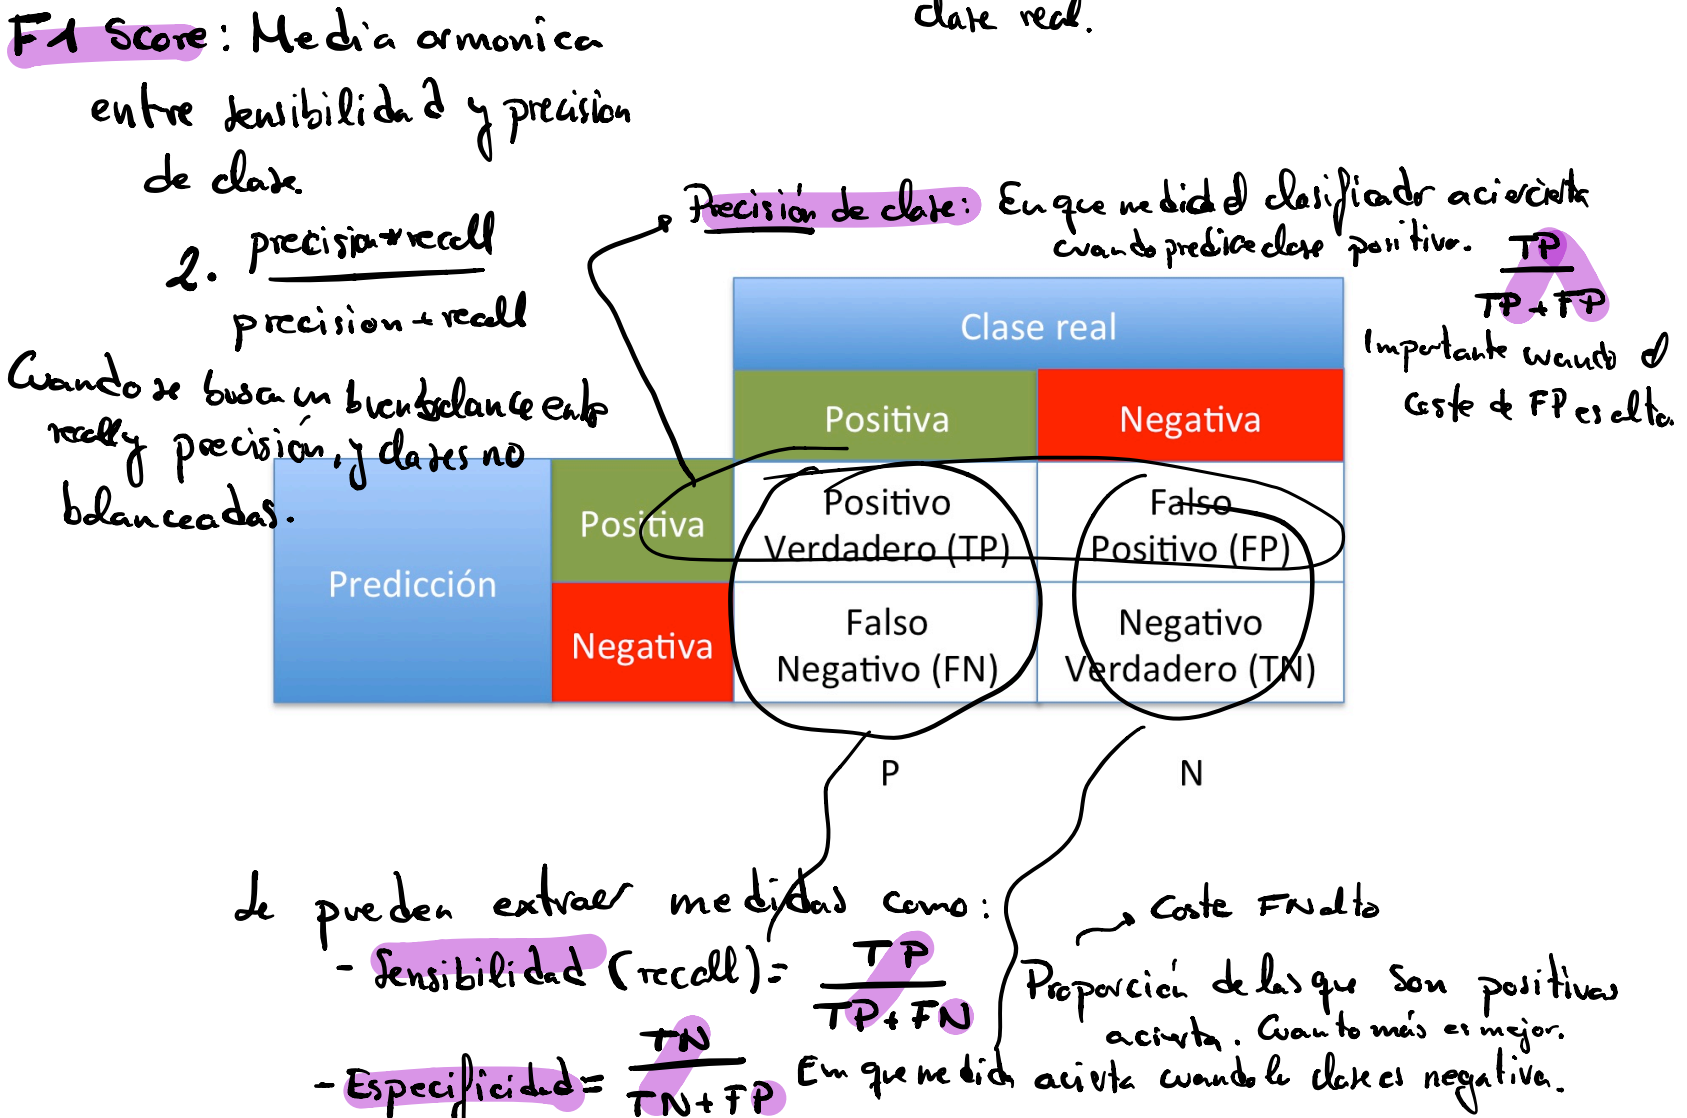
\includegraphics[scale=.2]{Untitled 11.png}}
\end{figure}

\(Accuracy= \frac {TP+TN}{TP+TP+FP+FN}\)

\(\textit{Sensibilidad(recall)}= \frac {TP}{TP+FN}\) Proporción de las que son
positivas acierta. Cuanto más es mejor.

Cuando el coste de FN es alto.

\(\textit{Especificidad}= \frac {TN}{TN+FP}\) En qué medida acierta cuando la
clase es negativa.

\(\textit{Tasa de falsos positivos}=1-\textit{Especificidad}= \frac {FP}{TN+FP}\)

\(\textit{Precision de clase}= \frac {TP}{TP+FP}\) En qué medida el
clasificador acierta cuando predice clase positiva.

Importante cuando el coste FP es alto.

\(\textit{F1 score}= 2\cdot \frac {precision \cdot recall}{precision +recall}\)
Medida armónica entre sensibilidad y precisión de clase.

Cuando se busca un buen balance entre recall y precisión de clase, y las
clases no balanceadas.
\newpage
\textbf{Espacio ROC:} Mide como de útil es un clasificador para
distinguir entre clases. Cuanto más cerca de la esquina superior
izquierda mejor, recoge más área y está más cerca del punto óptimo.
\begin{figure}[H]
	Ejemplo
	\ffigbox[\FBwidth]
	{\caption{Espacio ROC}}
	{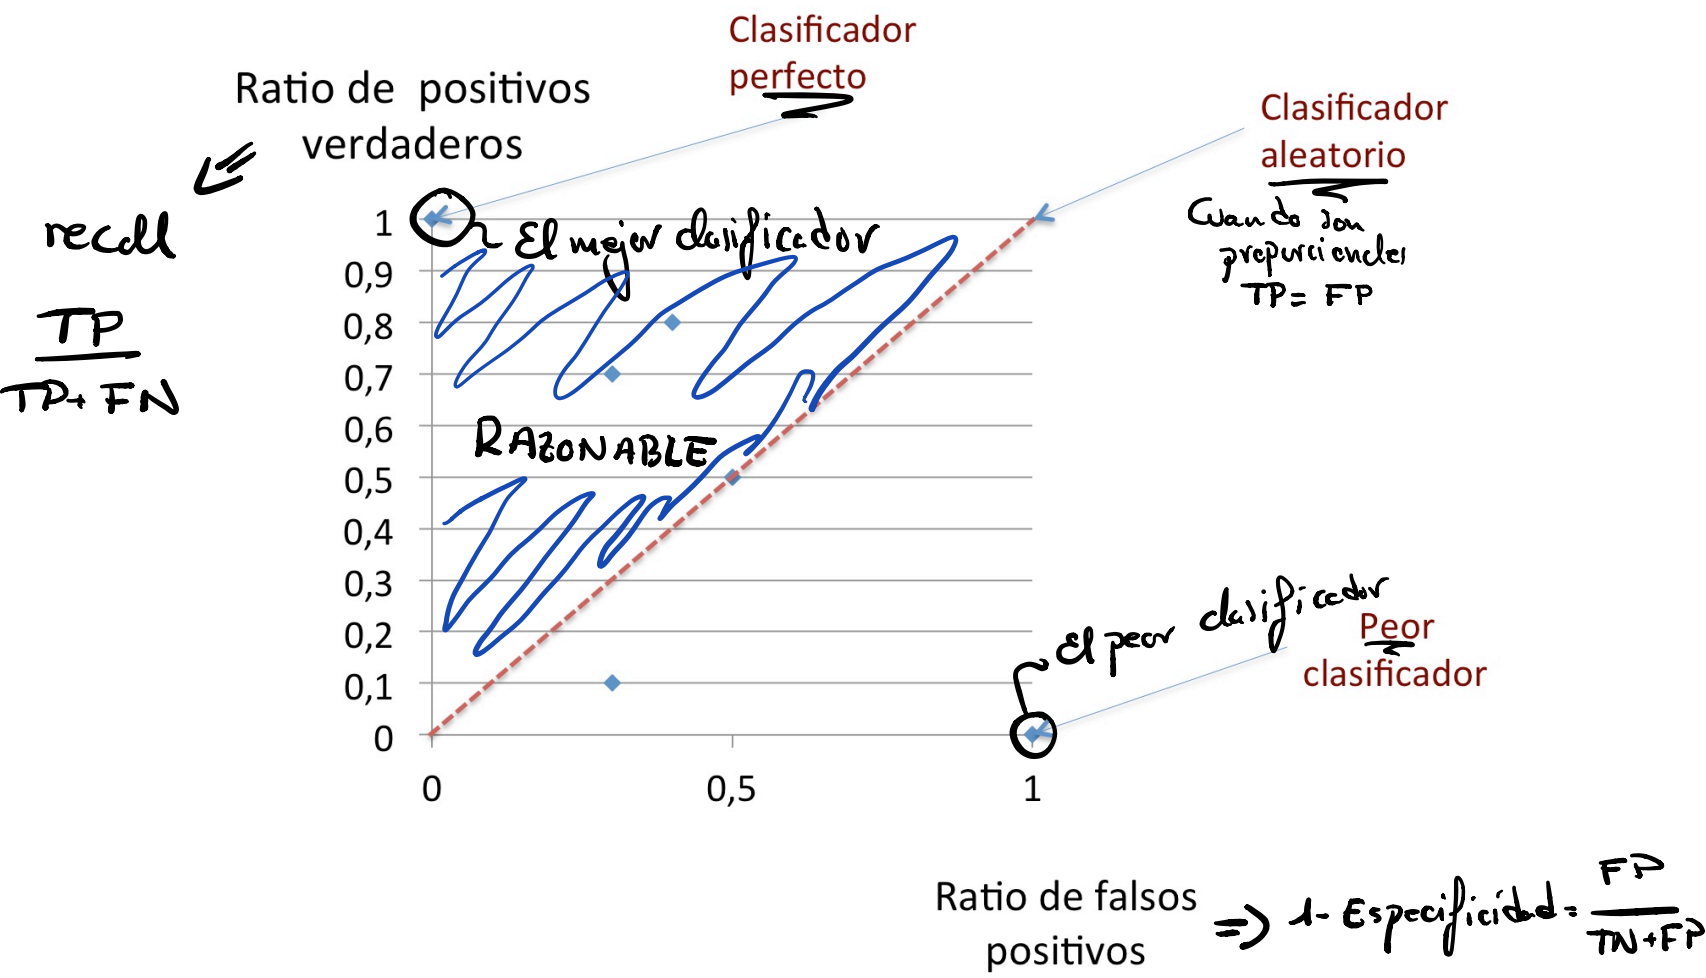
\includegraphics[scale=.2]{Untitled 12.png}}
\end{figure}
\textbf{Curva ROC}: Es una curva en el espacio ROC, en la que cada punto
de la recta representa un clasificador, el más cercano al punto óptimo
será el mejor, pero teniendo cuidado de los falsos positivos.

En el caso de árboles de decisión no lo utilizaremos porque no tiene 
sentido, pero si en los casos que hay que definir un umbral 
(Clasificador Bayesiano) a partir del cual se considera de clase positiva 
o negativa. Los puntos representan los distintos umbrales.

Cuanto más Área por debajo de la curva mejor.

\begin{figure}[H]
	\ffigbox[\FBwidth]
	{\caption{Curvas ROC}}
	{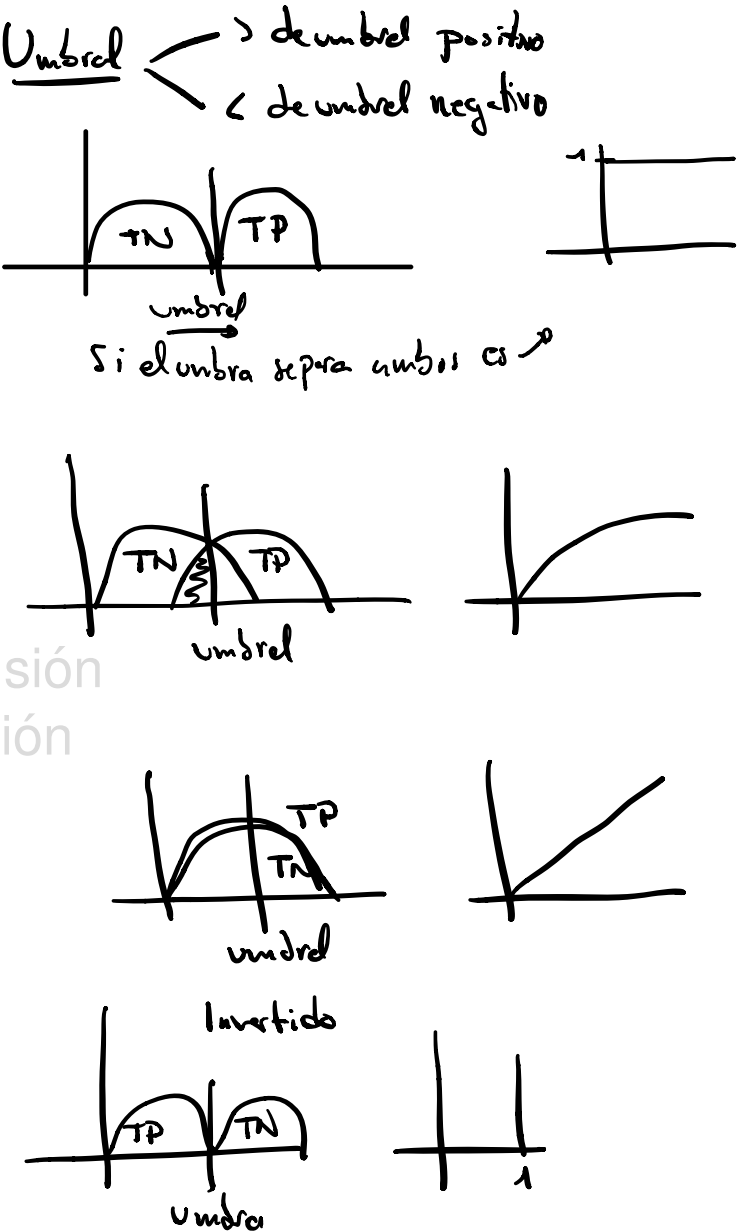
\includegraphics[scale=.18]{Untitled 13.png}}
\end{figure}

\section{Proceso de análisis de
datos}

Es un proceso iterativo, tras la última etapa se vuelve al principio.

\begin{enumerate}
\def\labelenumi{\arabic{enumi}.}
\item
  \textbf{Preprocesamiento}.

  \begin{itemize}
  \item
    \textbf{Tratamiento de datos imperfectos:}

    \begin{itemize}
    
    \item
      \textbf{Reducción del ruido:} Mediante filtros que eliminan
      instancias clasificadas mal.
    \item
      \textbf{Valores desconocidos:} Eliminar instancias/atributos o
      asignar el valor más probable.
    \end{itemize}
  \item
    \textbf{Reducción de datos:} Reducir la variedad.

    \begin{itemize}
    \item
      \textbf{Normalización}: Valores entre 0 y 1.
    \item
      \textbf{Discretización}: En rangos.
    \item
      \textbf{Selección de instancias}: Aleatoriamente, los más
      parecidos entre sí, los más diferentes entre sí o según alguna
      distribución.
    \item
      \textbf{Selección de atributos:}

      \begin{itemize}
      \item
        Reducción de la dimensionalidad de los datos, mediante filtrado
        según algún criterio o seleccionando un subconjunto.
      \item
        \textbf{Búsqueda}: Cualquier técnica.
      \item
        \textbf{Evaluación}: Correlación, entropía, etc.
      \item
        \textbf{Criterio de parada:} Porcentaje, umbral, iteraciones,
        etc.
      \item
        \textbf{Técnicas de wrapper}: Se genera el modelo con todos los
        atributos, se evalúa el modelo y se ve el subconjunto de
        atributos mejores.
		\begin{figure}[H]
			Ejemplo
			\ffigbox[\FBwidth]
			{\caption{Técnicas de wrapper}}
			{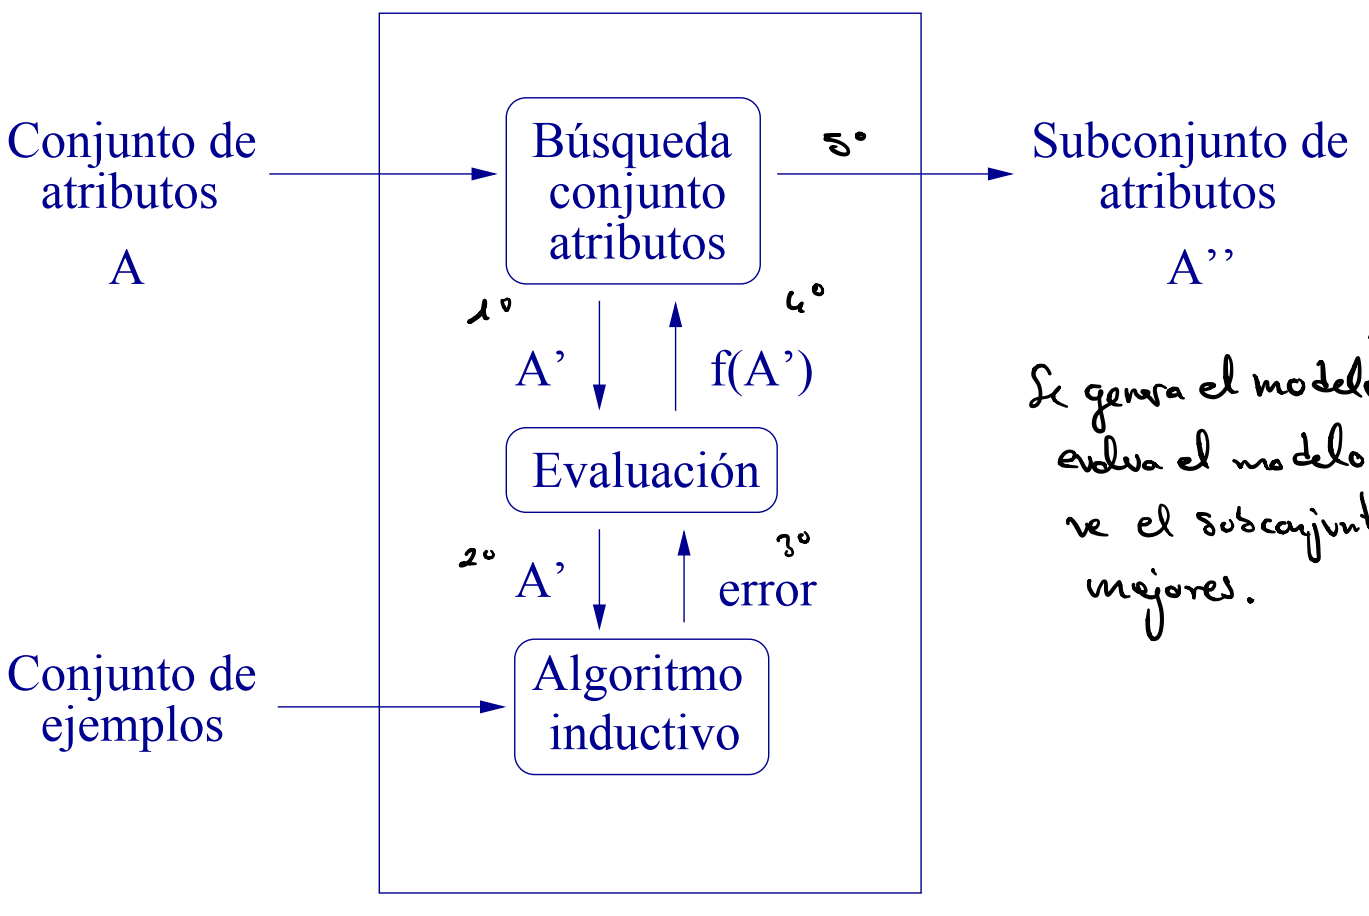
\includegraphics[scale=.2]{Untitled 14.png}}
		\end{figure}
    \pagebreak
      \item
        \textbf{Búsqueda en el espacio de estado de los conjuntos de
        atributos.}
		\begin{figure}[H]
			Ejemplo
			\ffigbox[\FBwidth]
			{\caption{Búsqueda por atributos}}
			{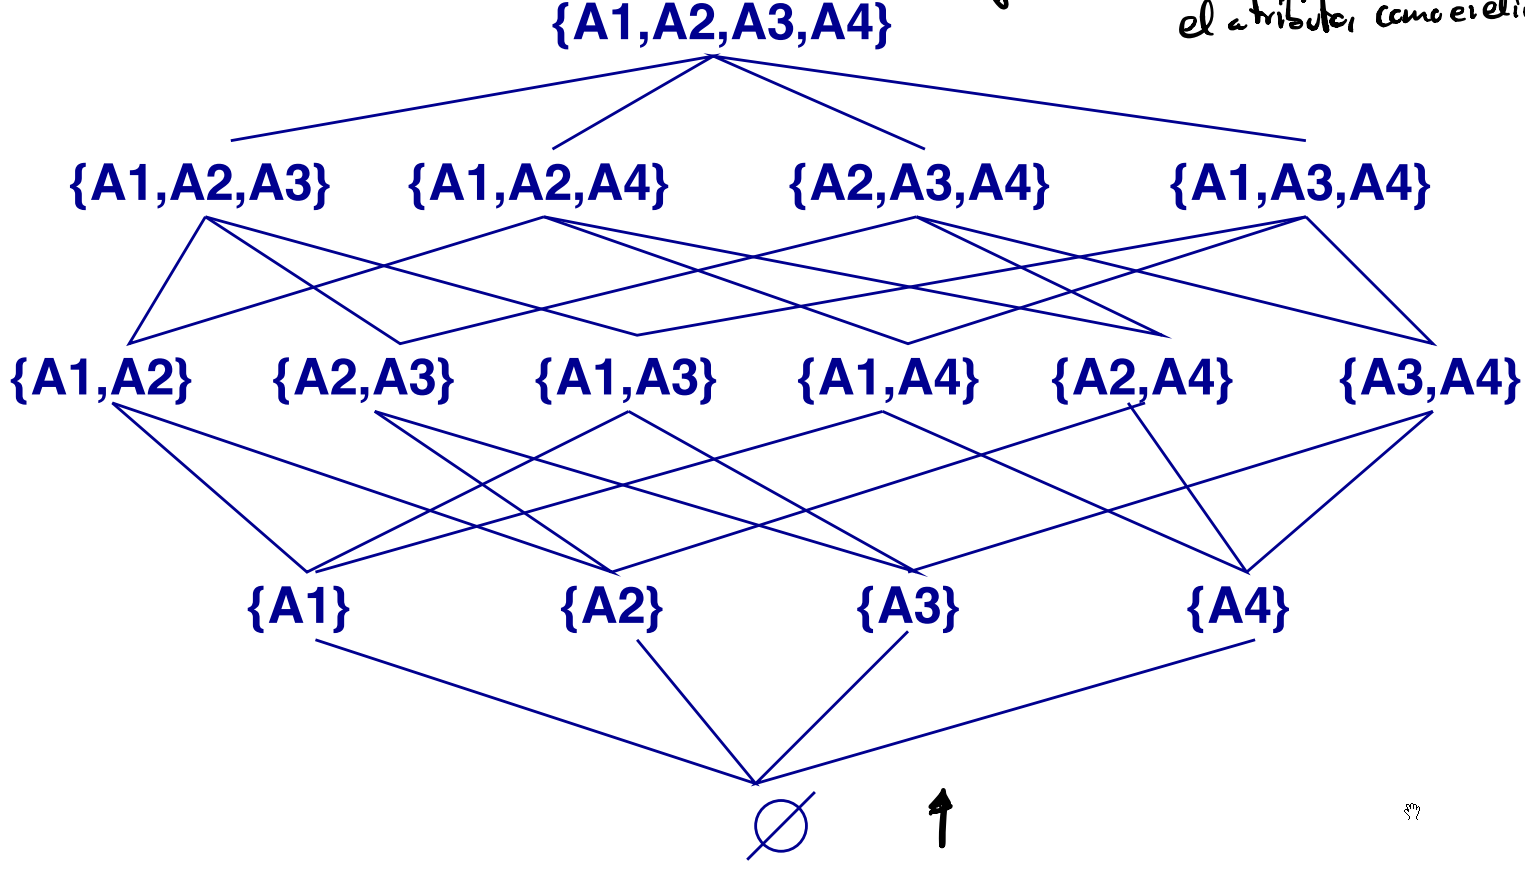
\includegraphics[scale=.15]{Untitled 15.png}}
		\end{figure}
        \begin{itemize}
        
        \item
          Se puede comenzar por el conjunto completo (por arriba) o por
          el conjunto vacío (por abajo).
        \item
          La búsqueda puede ser de cualquier tipo.
        \item
          La evaluación de cada nodo, que son subconjuntos de atributos,
          se realiza llamando al algoritmo inductivo seleccionado, una
          función de evaluación. Tras evaluar se opera.
        \end{itemize}
      \item
        \textbf{PCA (No lo usaremos):} Análisis de componentes
        principales. Es una solución algebraica, describe los datos en
        términos de nuevos atributos que no están correlados entre sí.
      \end{itemize}
    \item
      \textbf{Datos no balanceados:} Crear ejemplos sintéticos de la
      clase desbalanceada.
    \end{itemize}
  \end{itemize}
\item
  \textbf{Diseño}.

  \begin{itemize}
  
  \item
    Selección de algoritmo.
  \item
    Selección de parámetros.
  \end{itemize}
\item
  \textbf{Ejecución de algoritmo.}
\item
  \textbf{Postproceso.}

  \begin{itemize}
  
  \item
    Análisis de resultados.
  \item
    Visualización.
  \end{itemize}
\end{enumerate}

\section{Aspectos avanzados}

\subsection{Sobreajuste
(overfitting)}

\begin{figure}[H]
	Ejemplo
	\ffigbox[\FBwidth]
	{\caption{Diagrama de sobreajuste}}
	{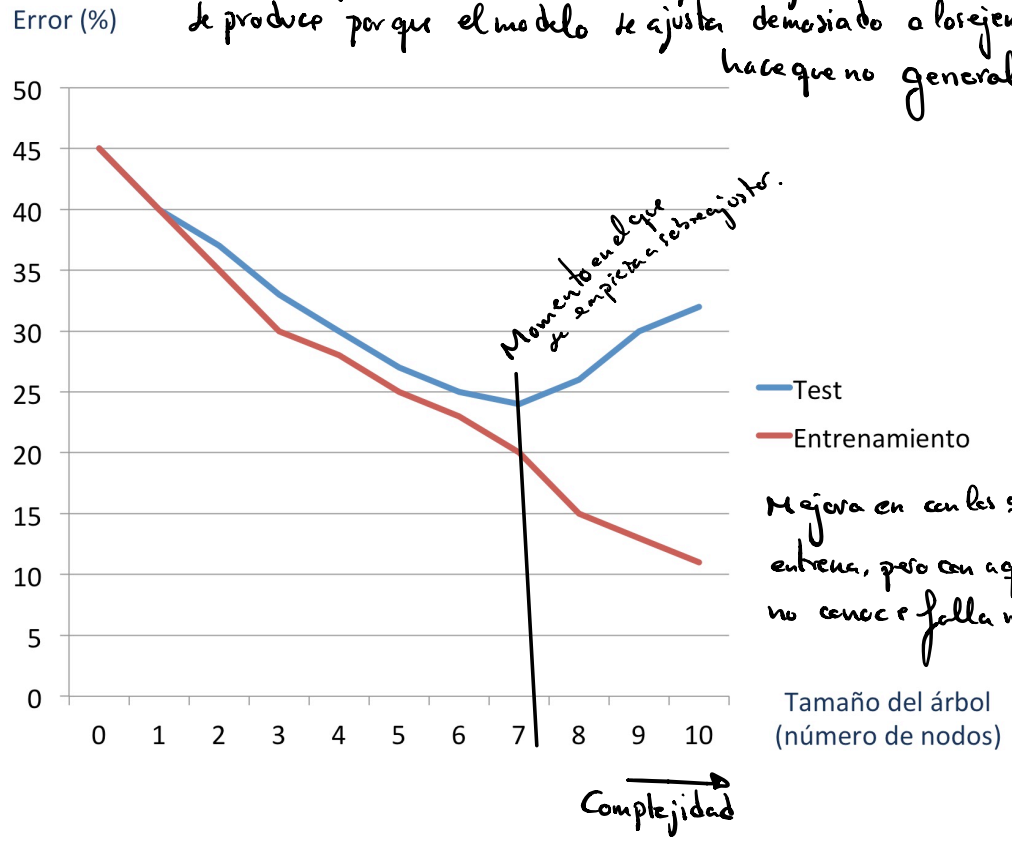
\includegraphics[scale=.2]{image-20210305195646416.png}}
\end{figure}

Fenómeno que se produce al hacer aprendizaje, porque \textbf{el modelo
se ajusta demasiado a los ejemplos, y eso hace que no generalice bien.}

Mejora con los que se entrena, pero con aquellas que no conoce falla
más.

Para evitar sobreajuste se debe generalizar, hay \textbf{2 métodos}:

\begin{itemize}
\item
  \textbf{Pre-poda}: Mientras se construye se poda.

  \begin{itemize}
  
  \item
    \textbf{Método de \(\chi^2\) (chi-cuadrado)}: Si en un nodo la
    diferencia entre clases no es significativa, no se divide, para con
    la mayoría. Muy conservador.
  \item
    \textbf{Mediante curvas de error}: Cross-validation. De esta manera
    podemos detectar el punto de inflexión, donde se empieza a producir
    overfitting (en el punto que se separan las curvas).
  \end{itemize}
\item
  \textbf{Post-poda}: Después de generar poda.

  \begin{itemize}
  \item
    \textbf{Eliminando subárboles}: Eliminando nodos del árbol empezando
    por las hojas, se evalúa el error tras eliminarlo, si no mejora
    probamos otro.
  \pagebreak
  \item
    \textbf{Eliminando precondiciones o reglas}: Tras haberlo pasado a
    reglas, eliminamos condiciones o reglas completas. Tras la
    eliminación se calcula el error, si mejora, el modelo principal pasa
    a ser el que lo eliminó y se sigue probado. Si no se prueba otra
    condición o regla.
	\begin{figure}[H]
		\ffigbox[\FBwidth]
		{\caption{Eliminación de atributos/reglas Post-poda}}
		{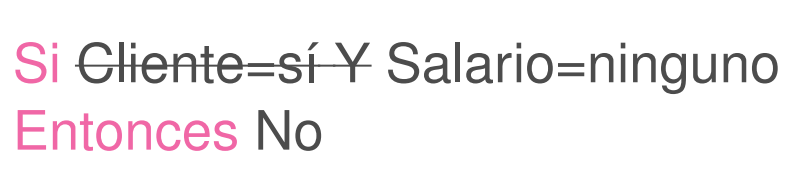
\includegraphics[scale=.2]{image-20210305201114245.png}
		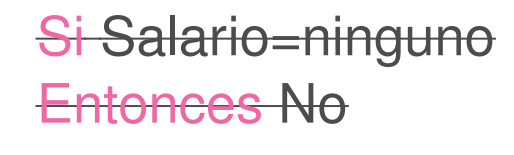
\includegraphics[scale=.2]{image-20210305201127523.png}}
	\end{figure}
  \end{itemize}
\end{itemize}

\subsection{Atributos con valores
continuos}
\begin{figure}[H]
	\ffigbox[\FBwidth]
	{\caption{Tratamiento de valores continuos}}
	{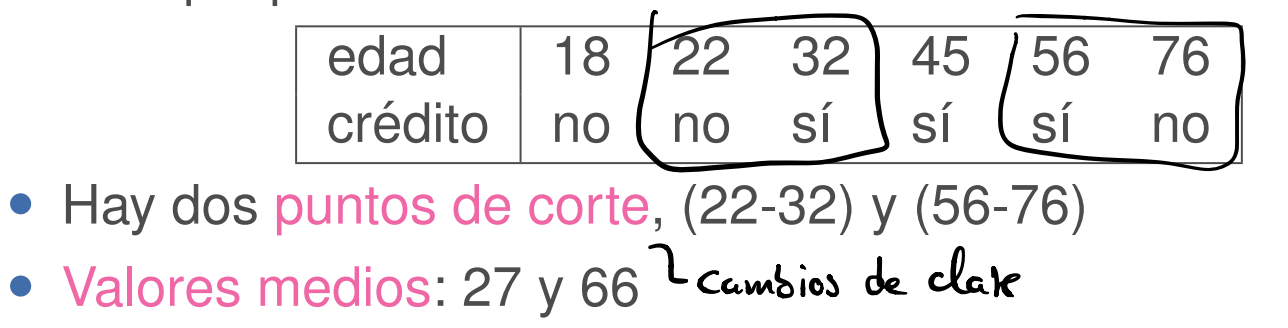
\includegraphics[scale=.2]{image-20210305201824512.png}}
\end{figure}

\begin{enumerate}
\def\labelenumi{\arabic{enumi}.}

\item
  Se \textbf{ordenan los valores del atributo}, y se especifica la clase
  a la que pertenecen.
\item
  Se \textbf{observan los puntos en los que pasa de una clase a otra} y
  se hace media con los puntos de corte.
\item
  Los \textbf{nodos de decisión se crean según:}

  \begin{itemize}
  
  \item
    Se trata como \textbf{atributo binario}: Se escoge \textbf{una sola
    regla de distinción} entre valores, el de mayor ganancia de
    información, que se eligen con los valores medios. Las reglas son del
    tipo atrib\textless punto1 o atrib\textless punto2.
  \item
    Se trata como \textbf{atributos multivaluado}: Se crean
    \textbf{tanto grupos como queramos}, lo más preciso es uno por cada
    intervalo de valores que tengan la misma clase.
  \end{itemize}
\end{enumerate}

\subsection{Atributos con muchos
valores}

\textbf{ID3 prefiere atributos con mayor número de valores.}

\textbf{Problema}: Que cada uno puede tener un valor único, y no se podrá usar para clasificar.

\textbf{Alternativas}:

\begin{itemize}

\item
  Por cada valor v del atributo A, se puede \textbf{crear un atributo binario}, de si ese atributo toma ese valor o no.
  \pagebreak
\item \textbf{Razón de ganancia (GainRatio, GR)}: Ganancia calculada como la ganancia partida por una penalización por el número de valores del
  atributos.
  \begin{figure}[H]
    $$
    GR(S, A)= \frac {G(S, A)=max Entropia(S)-EntropiaAtrib(S, A)}{\textit{Split\_Information}(S, A)=-\sum_{v\in valores(A)} \frac {|S_v|}{|S|} \cdot log_2(\frac {|S_v|}{|S|})}
    $$
    \captionsetup{justification=centering}
    \caption{Razón de ganancia}
  \end{figure}
  $$
  \textit{Split\_Information}(S, A)=-\sum_{v\in valores(A)} \frac {|S_v|}{|S|} \cdot log_2(\frac {|S_v|}{|S|}) 
  $$
\end{itemize}

\subsection{Atributos con costes
variables}

Como podrían ser pruebas médicas caras, obtener los ejemplos es caro.
\textbf{Consiste en penalizar la entropía de los atributos con coste
variable.}

\(\frac {G(S, A)}{unidad \space de \space coste(A)} o \frac {G(S, A)}{unidad \space de \space coste(A)^2}\)

\section{Otras alternativas a ID3}

\textbf{Clasificadores débiles:}

\begin{itemize}

\item
  \textbf{ZeroR}: En clasificación, dará siempre la \textbf{clase más
  frecuente}, la moda de la clase. En regresión, devuelve la media.
\item
  \textbf{OneR}: Construye un conjunto de \textbf{reglas de decisión con
  un solo atributo}. Se elige aquel atributo con menor error, para cada
  valor del atributo se crea una regla, donde el valor que toma es el
  más frecuente.
\end{itemize}

\section{Implementaciones}

\begin{description}
	\item[ID3, 1986]
	\item[C4.5, 1993] Sucesor de ID3, atributos numéricos, conversación a reglas, poda.
	\item[C5.0] Versión comercial.
	\item[J48] Implementación JAVA de C4.5.
\end{description}

\chapter{Tema 3: Regresión}
\begin{figure}[H]
	\ffigbox[\FBwidth]
	{\caption{Ejemplo instancias de Regresión}}
	{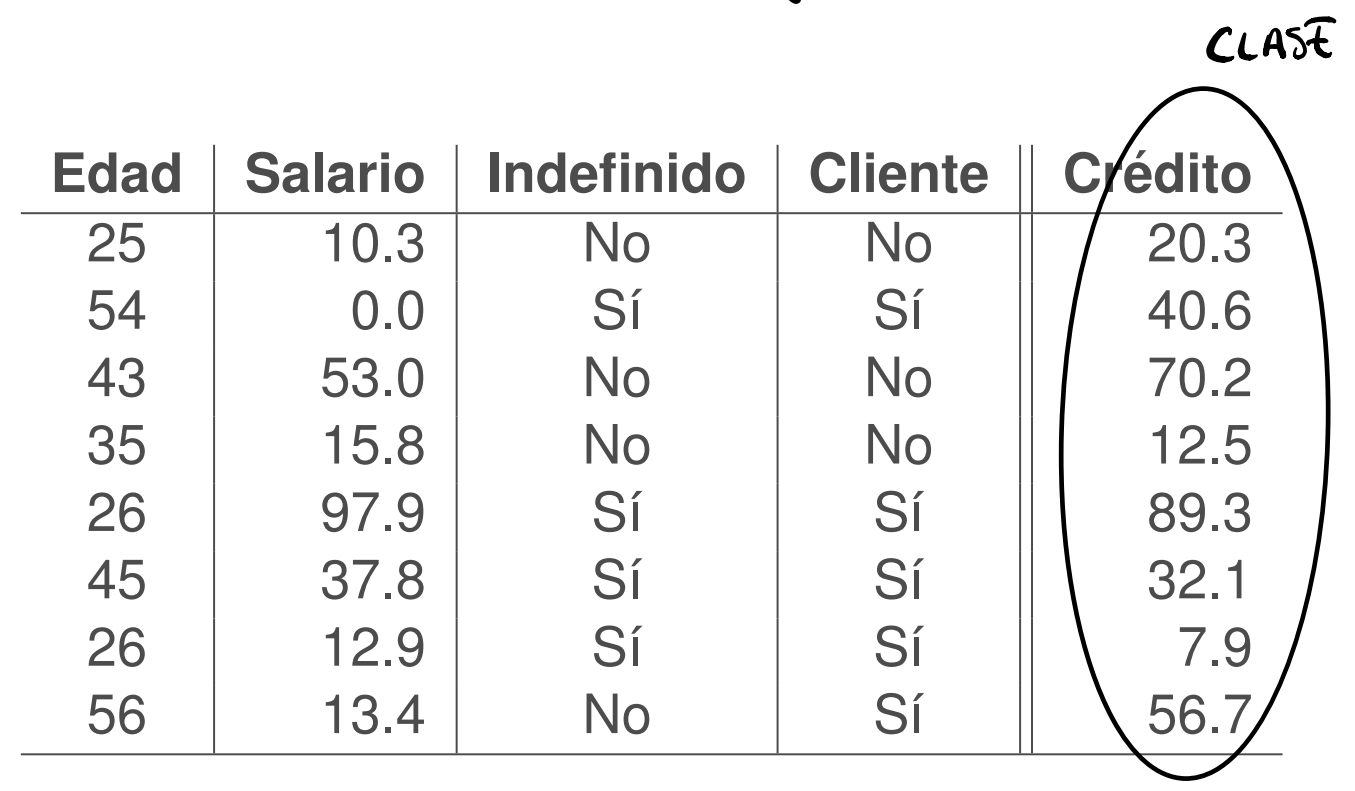
\includegraphics[scale=.2]{image-20210305210244509.png}}
\end{figure}
La clase en regresión es numérica.

\section{Regresión como
clasificación}

Discretizando la clase, pero se pierde información y hay que elegir un
método de discretización.

\textbf{Soluciones}:

\begin{itemize}

\item
  \textbf{Discretización de clase.}
\item
  \textbf{Discretización fija.}
\item
  \textbf{Discretización dinámica.}
\end{itemize}

\section{Función de regresión}
\begin{figure}[H]
	\ffigbox[\FBwidth]
	{\caption{Ejemplo Regresión Lineal}}
	{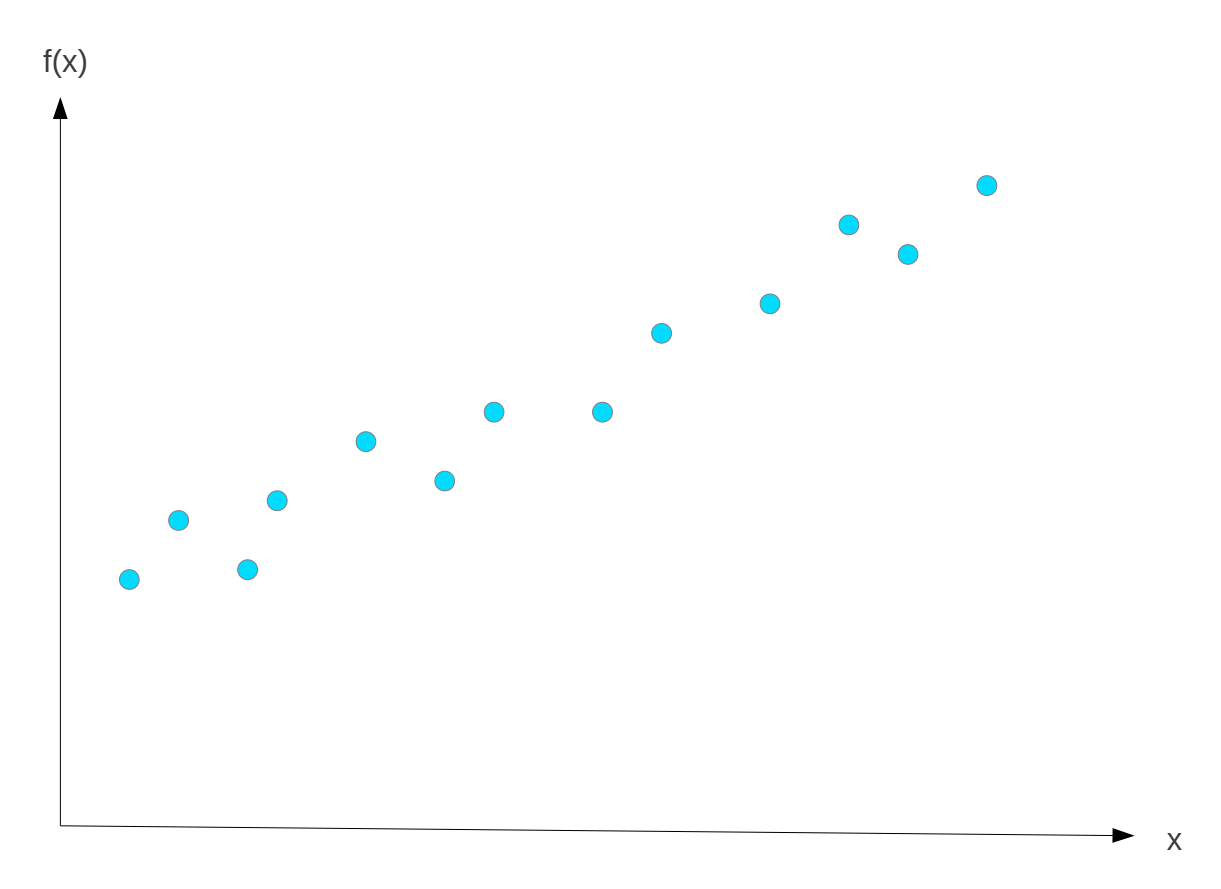
\includegraphics[scale=.15]{image-20210305211354068.png}
	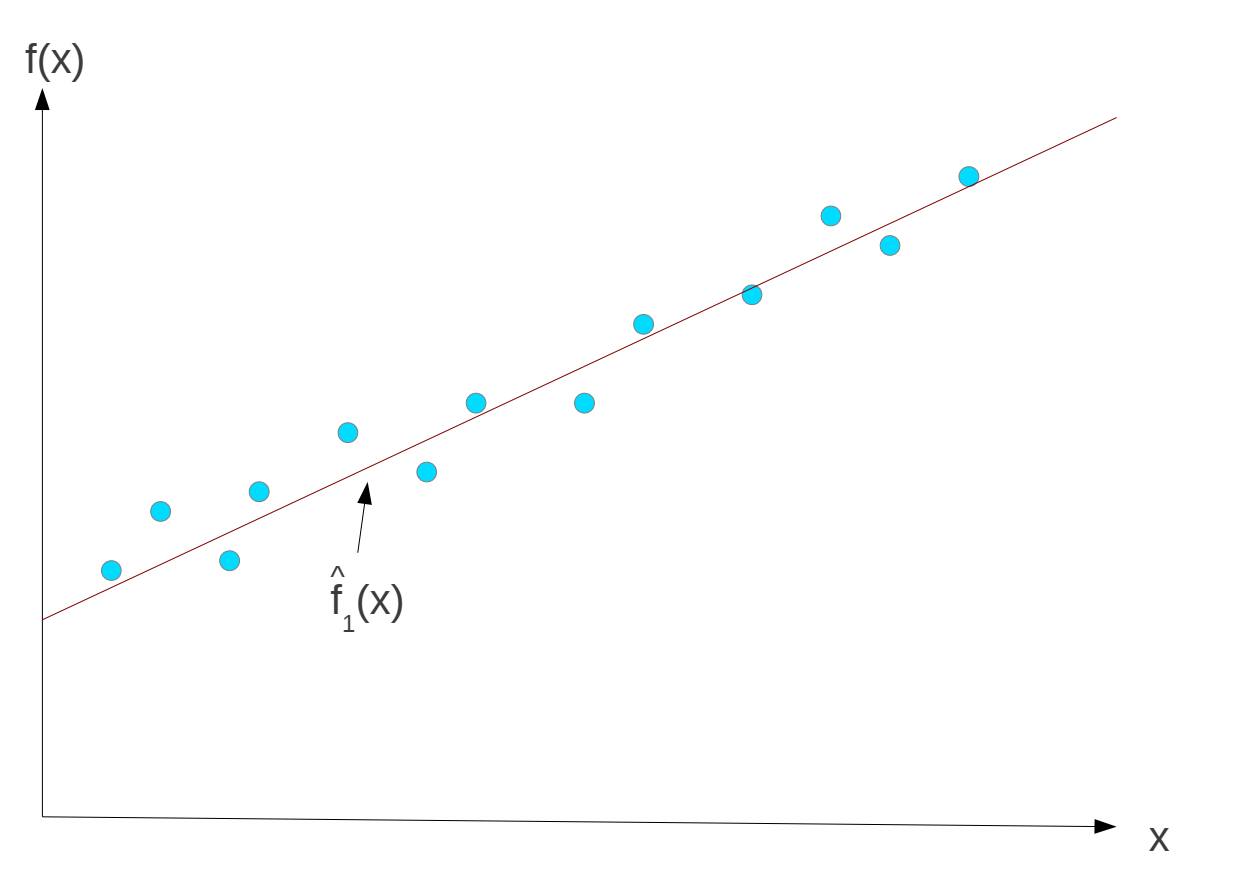
\includegraphics[scale=.15]{image-20210305211454026.png}}
\end{figure}

\subsection{Regresión lineal}

Hallar una \textbf{función que se ajuste lo mejor posible a la nube de
puntos}. En el caso de la \textbf{lineal es una recta.}

Aproximar una función \(f(x)\) que no tiene por qué ser lineal en
regresión, con una función
\textbf{\(\hat{f}(x)= w_0 + w_1a_1(x)+ w_2a_2(x)+ ...+ w_na_n(x)\)}
donde

\begin{itemize}

\item
  \(a_i\) denota el \textbf{atributo} i-ésimo del ejemplo x.
\item
  \(w_i\) \textbf{peso} del atributo
\end{itemize}

\textbf{Objetivo}: Encontrar aquellos \(w_i\) que minimicen el error
entre la función clase y el valor de la aproximación.

Equivalente a \textbf{minimizar el error cuadrático sobre el conjunto de
entrenamiento total, } C: \(E= \sum _{c \in C} (f(x)-\hat{f}(x))^2\) Lo
que queremos es minimizar.

\subsection{Error de Regresión}

La \textbf{suma de todas las diferencias de los valores de la función y
su aproximación}. Buscamos aquella aproximación que minimice E.
\begin{figure}[H]
	\ffigbox[\FBwidth]
	{\caption{Error en Regresión Lineal}}
	{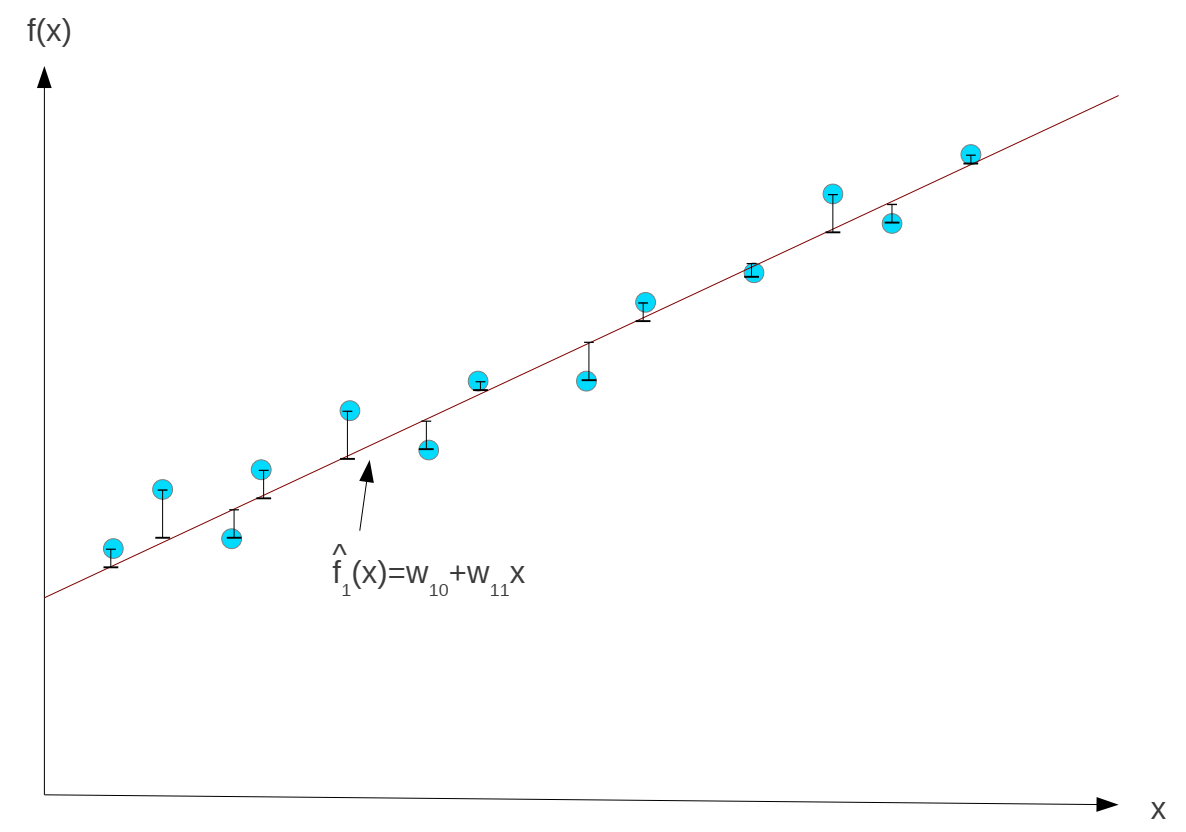
\includegraphics[scale=.10]{image-20210305212854142.png}}
\end{figure}

\subsubsection{Minimizando el error}

\textbf{El problema de definir la función se traslada a un problema de
definir el vector de pesos w.} Se debe encontrar el vector \(\vec{w}\)
que minimice la función de error, problema de búsqueda en el espacio de
pesos.

\textbf{Aproximación}: Descenso de gradiente.

\subsection{Descenso de gradiente}
\begin{figure}[H]
	\ffigbox[\FBwidth]
	{\caption{Diagrama de Descenso de Gradiente}}
	{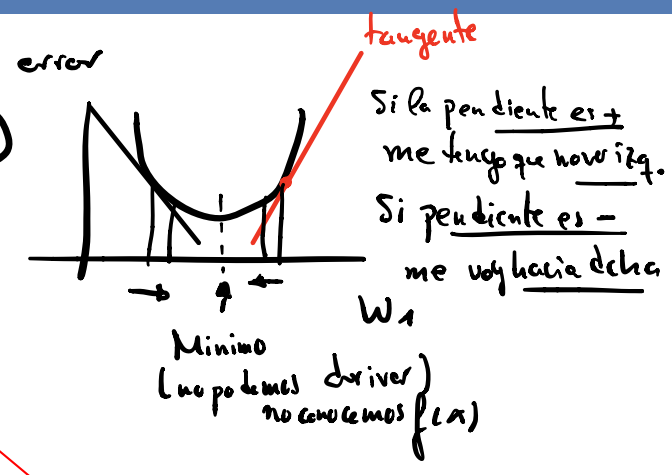
\includegraphics[scale=.3]{image-20210305214445428.png}}
\end{figure}
Sobre la función de errores por variable \textbf{vamos calculando la tangente y desplazando los valores de los pesos}.

\begin{itemize}

\item
  Consisten en movernos poco a poco en los pesos, para no pasarnos, y se parte de pesos aleatorios.
\item
  Si la \textbf{tangente} tiene pendiente \textbf{positiva}, nos
  desplazamos a la \textbf{izquierda}.
\item
  Si la \textbf{tangente} tiene pendiente \textbf{negativa}, vamos a la
  \textbf{derecha}.
\end{itemize}

\textbf{Gradiente del error respecto a w:} Derivada parcial de la
función de error de cada uno de los pesos.
\(\nabla E[\vec{w}] \equiv\left[\frac{\partial E}{\partial w_{0}}, \frac{\partial E}{\partial w_{1}}, \cdots ,\frac{\partial E}{\partial w_{n}}\right]\)

\textbf{Regla de entrenamiento:}
\(\Delta \vec{w}=-\eta \nabla E[\vec{w}]\)

\textbf{Derivada del error:}
\(\frac{\partial E}{\partial w_{i}}=\sum_{e}\left(t_{e}-o_{e}\right)\left(-x_{i, e}\right)\)

\begin{itemize}

\item
  \(t_e\): Valor \textbf{verdadero} para la instancia e.
\item
  \(o_e\): Valor de \textbf{salida del modelo} para la instancia e.
\item
  \(x_{i,e}\): Valor del \textbf{atributo} a para la instancia e.
\end{itemize}
\pagebreak
\textbf{Procedimiento: Descenso de Gradiente(C, n)}

\begin{itemize}

\item
  C conjunto de ejemplo de entrenamiento. n tasa de aprendizaje cuando
  salta.
\end{itemize}

\begin{figure}[H]
	\ffigbox[\FBwidth]
	{\caption{Algoritmo de Descenso de Gradiente}}
	{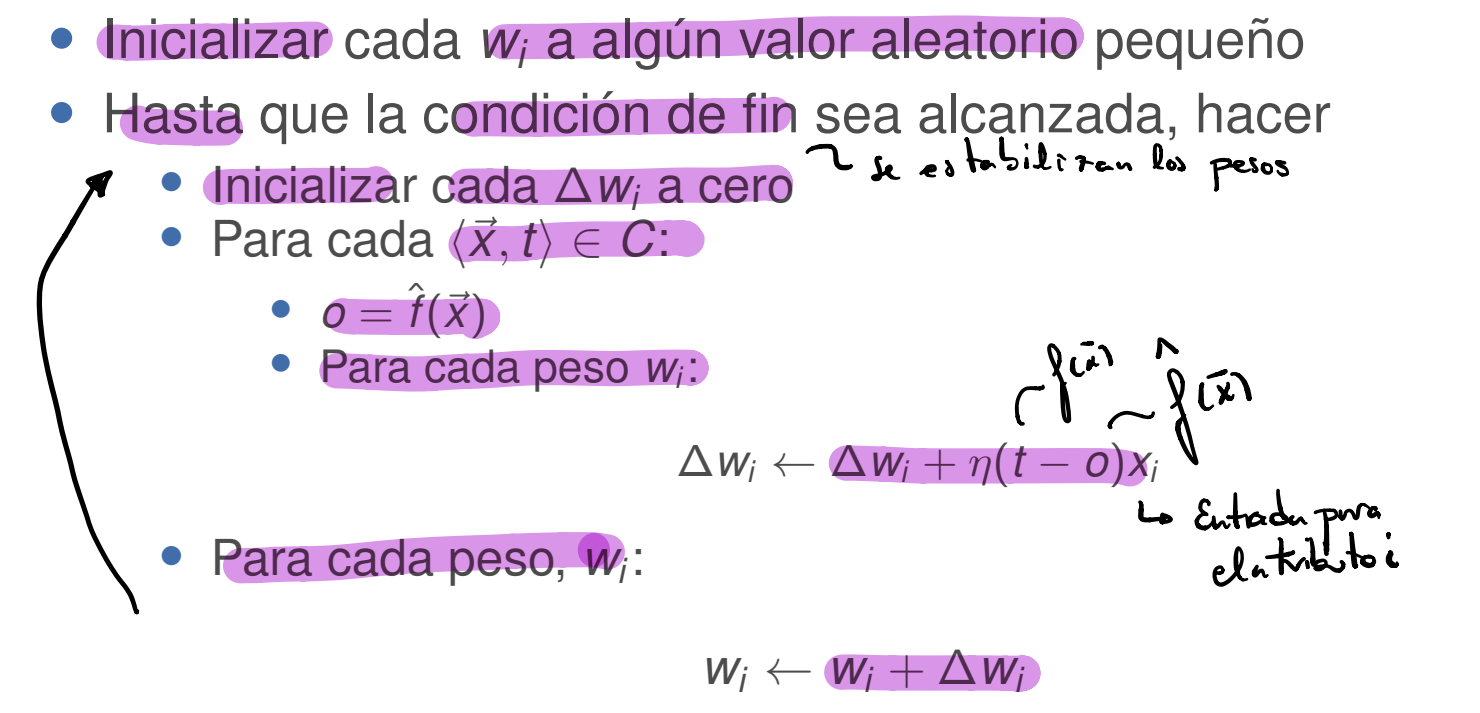
\includegraphics[scale=.2]{image-20210305224415026.png}}
\end{figure}

\subsection{Regresión no lineal}

Cuando usamos este tipo de funciones hay que tener \textbf{cuidado}, la
evaluación se debe realizar con ejemplos de un conjunto distinto al de
entrenamiento, porque la función no lineal se puede ajustar muy bien a
esos, pero no al resto.

Esta función es más difícil de generar.

\section{Regresión paramétrica}

Elegir una función lineal, logística o cualquier tipo, para que se ajuste.

El modelo o predictor adopta una forma predeterminada.

Regresión lineal es regresión paramétrica. También se puede hacer
regresión no lineal paramétrica, función logística, polinómica, etc.

\section{Árboles de regresión}

Regresión no lineal y no paramétrica.

\section{M5}

\textbf{M5 es una variación de CART}, donde las hojas son valores numéricos y
elige aquel atributo que maximice la reducción esperada en varianza.

\textbf{Estrategia}: Se divide el espacio en partes y hace regresión
lineal por partes, no global.

\textbf{Algoritmo}: Parecido a ID3, pero en este caso se trata de
reducir la variación interna de los valores de la clase de cada
subconjunto.

\begin{itemize}
\item
  Elige aquel atributo que maximice la reducción del error (en vez de
  entropía o desviación típica). Nos quedamos con la menor media de
  desviaciones.
  \begin{figure}[H]
    \(\Delta \operatorname{error}(S, A)=\operatorname{sd}(S)-\sum_{v \in \text { valoresTestNodo }(A)} \frac{\left|S_{A=v}\right|}{|S|} \times \operatorname{sd}\left(S_{A=v}\right)\)
    \captionsetup{justification=centering}
    \caption{Formula desviación M5}
  \end{figure}

  \begin{itemize}
  
  \item
    \textbf{S} conjunto de ejemplos en el nodo a dividir.
  \item
    \textbf{\(S_{A=v}\)} Ejemplos con valor v en el atributo A.
  \item
    \textbf{sd(S)} Desviación típica de los valores de la clase para los
    ejemplos en S.
  \end{itemize}
\end{itemize}

\textbf{Criterio de parada}: Pocos ejemplos o poca variación de los
valores (desviación típica pequeña)

\textbf{Hojas}: Se calcula un modelo lineal y se utiliza regresión
estándar.

\textbf{Salida}: En las hojas tiene funciones de regresión, en los nodos
no hoja se tienen atributos acotados \textless. Cada nodo tiene un
conjunto de entrenamiento y se hace su regresión lineal.

\begin{figure}[H]
	\ffigbox[\FBwidth]
	{\caption{Diagramas M5}}
	{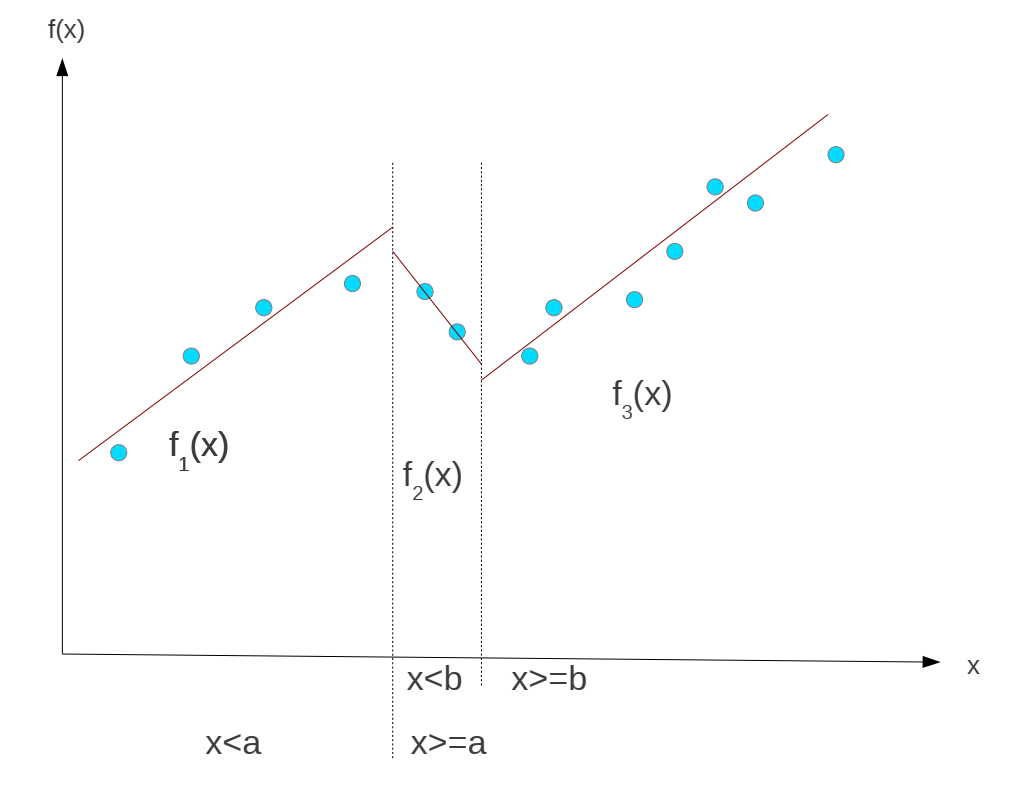
\includegraphics[scale=.2]{image-20210305230339091.png}
	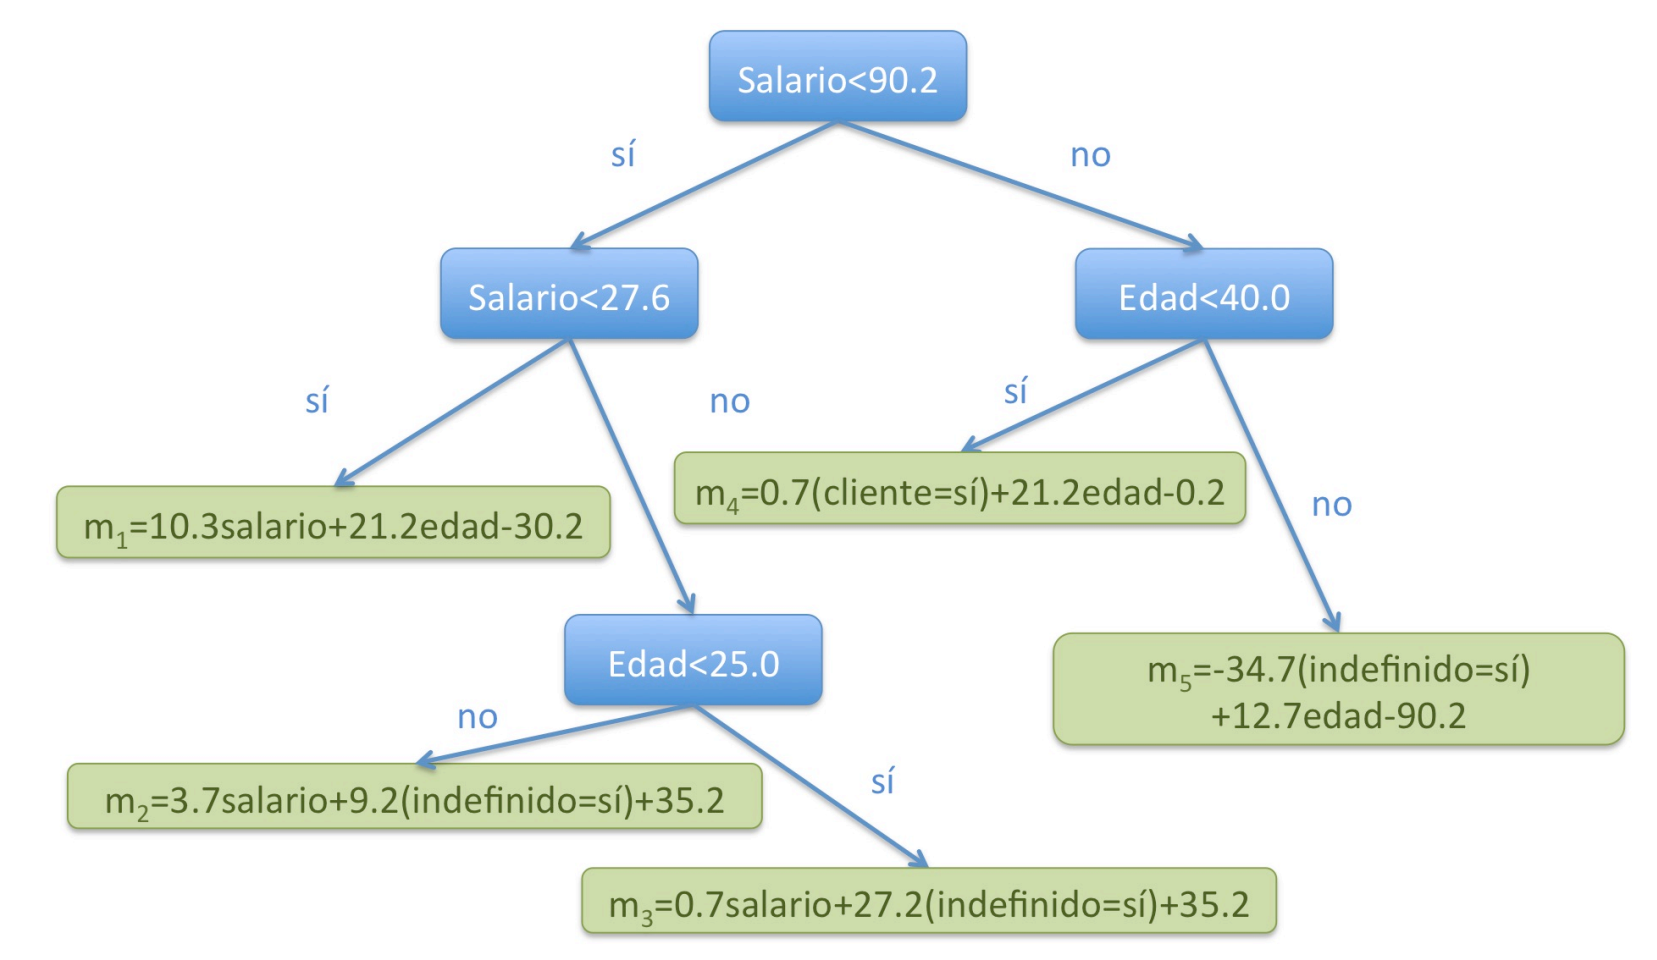
\includegraphics[scale=.15]{image-20210305230601935.png}}
\end{figure}
En los árboles de regresión, los nodos hoja tienen modelos lineales y
para llegar a esos nodos se usa como heurística la Desviación típica
(cuanto menor mejor), que se calcula haciendo una media ponderada
(\(S_{S=si}\cdot\frac {|S_{S=si}|}{|S|}\)) de las desviaciones típicas
de cada uno de los conjuntos resultantes.

Tras la construcción del árbol hay un proceso de poda, que consiste en
Simplificar los modelos lineales de las hojas, Simplificar el árbol para
que sea más pequeño y por último el Suavizado.
\pagebreak
\section{Poda}

\textbf{Paso 0}: Antes de realizar la poda se crean modelos lineales de los nodos
intermedios, que se utilizaran para ver si se pueden simplificar los subárboles por ese modelo del nodo intermedio. Para estos modelos se usan solo los atributos que aparecen en el subárbol.

Para decidir si simplificamos por un modelo lineal necesitamos una
medida del error. Si el modelo lineal proporciona menor error con
respecto al subárbol podemos simplificarlo utilizando el modelo.

La medida de error que empleamos es el \textbf{Error absoluto medio},
que es la media del error al clasificar las instancias el subconjunto de
instancias de entrenamiento del subárbol. Se calcula como $residuo(T) = \frac 1 n \sum _{i \in T} ||f(i)- \hat{f}(i)||$, dado un
subárbol con un subconjunto de n instancias de entrenamiento T.

El residuo subestima el error en instancias nuevas (que no ha visto
nunca), para solucionar esto se multiplica por
\(\alpha = \frac {n+v}{n-v}\). Tal que n es el número de ejemplos del
subárbol y v el número de atributos del modelo.

Por lo que el error aumenta cuando hay muchos parámetros o hay pocas
instancias.

\textbf{Formula del error:}
\(error\_estimado(T) = \alpha \times residuo(T)\) Es una proporción del
residuo.

\begin{enumerate}
\def\labelenumi{\arabic{enumi}.}
\item
  \textbf{Simplificación de los modelos lineales} (Busca eliminar
  atributos)

  Se realiza en cada modelo lineal. Se eliminan atributos, que se seleccionan utilizando escalada para reducir el error estimado. En el extremo, deja solo una constante, como termino independiente.

  \(M= 0.25a_1+0.12a_2+300a_5-40 \Rightarrow M=0.12a_2+300a_5-40\)
\item
\textbf{Simplificación del subárbol} (Busca eliminar subárboles por modelos
  lineales)

  Cada nodo interno del árbol tiene un modelo lineal simplificado y un
  modelo subárbol, y se elige aquel que minimice el error estimado. Si
  el modelo da mejor resultado, se sustituye el subárbol por el nodo del
  modelo.
\item
  \textbf{Suavizar el árbol}

  Algunos trabajos han comprobado que realizar un suavizado mejora la predicción final, dado que la predicción en cada nodo puede variar
  mucho. Lo que hace es en lugar de devolver la predicción del modelo en
  el nodo hoja, se consideran también los modelos en los nodos
  intermedios entre el nodo hoja y el nodo raíz.
\end{enumerate}

\chapter{Tema 4: Otras técnicas}

\section{Aprendizaje Bayesiano}

Funcionan bien en la clasificación de textos, text mining. Permite
recibir los datos de manera incremental y va creciendo el modelo.

\subsection{Hipótesis más probable
(MAP)}

Se busca la hipótesis que explique mejor los datos.
\begin{figure}[H]
  \[P(h_i/E)= \frac {P(E/h_i)P(h_i)}{P(E)}\]
  \captionsetup{justification=centering}
  \caption{Formula Hipótesis más probable}
\end{figure}

Es aquella que \(\arg \max P(h_i/E)\) o $\arg \max P(E/h_i) $.
Cogemos el \(h_i\) más probable, pero puede haber otros muchos modelos
que dicen que no y que habría que considerar, entonces lo que queremos
es la clase más probable para esos datos.

\subsection{Clasificación más
probable}

Probabilidad de la clase C dados los ejemplos E:
\begin{figure}[H]
  \(P(C/E) = \sum _{h_i \in H} P(C/h_i) \cdot P(h_i/E)\)
  \captionsetup{justification=centering}
  \caption{Formula Clase más probable}
\end{figure}

A esto se le llama \textbf{Clasificador Bayesiano Óptimo}, en la práctica el tamaño de H hace que sea imposible, además no tenemos un modelo como tal sino la probabilidad de la clase más probable para esos datos.

\subsection{Naïve Bayes}

\begin{figure}[H]
  \(\arg \max P(C/a_1, ...,a_n)= \arg \max _{c \in C} \frac {P(a_1, ...,a_n/C)P(C)}{P(a_1, ...,a_n)}=\arg \max_{c \in C} P(a_1, ...,a_n/C)P(C)\)
  \captionsetup{justification=centering}
  \caption{Fórmula Naïve Bayes}
\end{figure}

Podemos quitar el denominador porque todas las clases se evalúan con los
mismos atributos. Y \(P(a_1, ...,a_n/C)\) es muy complejo de calcular,
exponencial, se necesitaría una tabla de todas las combinaciones.

Para evitar esta complejidad se hace una simplificación, \textbf{se asume que los valores de los atributos una vez se conoce la clase son
condicionalmente independientes}, lo que quiere decir que se puede
calcular como un producto.
\(P(a_1, ...,a_n/C) = P(a_1/C) \cdot P(a_2/C) \cdot ... \cdot P(a_n/C) \cdot P(C)\).
El problema es que ahora es una aproximación y no un clasificador
bayesiano óptimo. \textbf{Suele funcionar bastante bien} esta
aproximación.

\(P(c=c_1)= \frac {n\_casos\_c=1}{n\_casosTotales}\)
\(P(a=v_1/c=c_1)= \frac {n\_casos\_c=1\_y\_v=v_1}{n\_casos\_c=1}\)

\section{Redes de neuronas}

\subsection{Neurona}

\begin{figure}[H]
	\ffigbox[\FBwidth]
	{\caption{Diagrama de una neurona}}
	{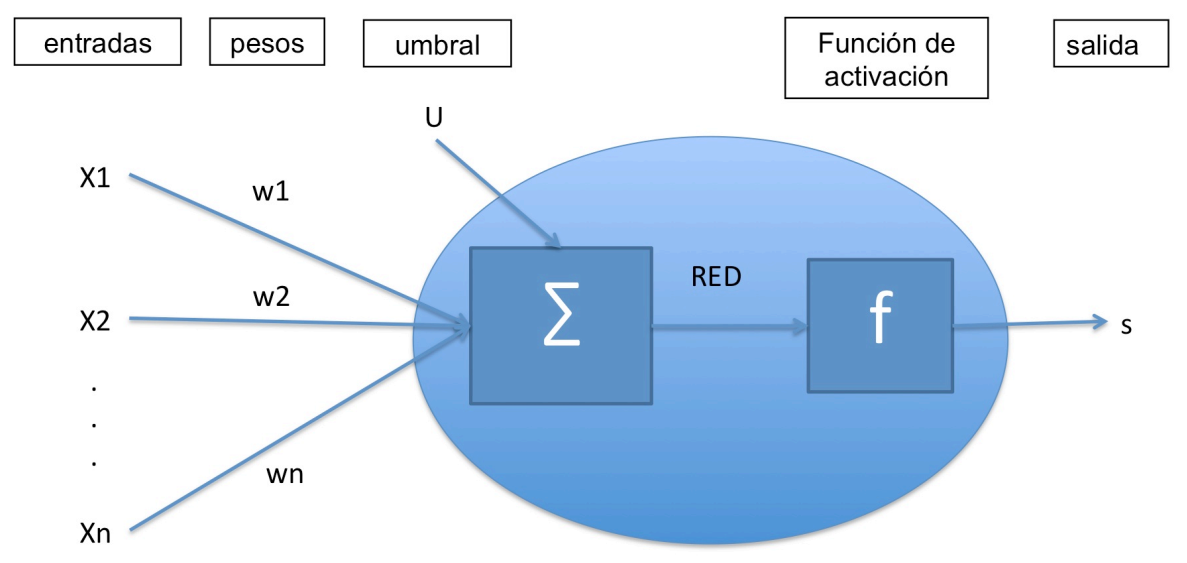
\includegraphics[scale=.2]{image-20210312101135112.png}}
\end{figure}
Las \textbf{entradas son los valores de los atributos}
(\(x_1,x_2,..,x_n\)) y un umbral, se hace \textbf{combinación lineal de
las entradas con unos pesos} (\(w_0+w_1x_1+...+w_nx_n\)) y se pasa el
\textbf{resultado por una función de activación} que nos da la salida.

\textbf{Tipos de función de activación:}
  \begin{figure}[H]
    \ffigbox[\FBwidth]
    {\caption{Función Umbral}}
    {\begin{tikzpicture}[scale=.5]
      \begin{axis}[
      	title={Función Umbral},
        xlabel={$x$},
        ylabel={$y$},
        legend pos=north west,
        ymajorgrids=true,
        xmajorgrids=true,
        grid style=dashed,
        axis lines=middle,
        xmin=-1, xmax=1, ymin=-1.5, ymax=1.5,
        axis x line=center,
        axis y line=center,
      ]
      \addplot [thick, color=blue] plot coordinates
      {
          (-1, -1)
          (0, -1)
          (0, 0)
          (0, 1)
          (1, 1)
      };
      \legend{Función}
        
      \end{axis}
    \end{tikzpicture}
    \begin{tikzpicture}[scale=.5]
      \begin{axis}[
        title={Función Lineal},
        xlabel={$x$},
        ylabel={$y$},
        legend pos=north west,
        ymajorgrids=true,
        xmajorgrids=true,
        grid style=dashed,
        axis lines=middle,
        xmin=-2, xmax=2, ymin=-2, ymax=2,
        axis x line=center,
        axis y line=center,
      ]
      \addplot[thick, color=blue]
        {x};
        \legend{Función}
        
      \end{axis}
    \end{tikzpicture}
    \begin{tikzpicture}[scale=.5]
      \begin{axis}[
        title={Función Sigmoide},
        xlabel={$x$},
        ylabel={$y$},
        legend pos=north west,
        ymajorgrids=true,
        xmajorgrids=true,
        grid style=dashed,
        axis lines=middle,
        axis x line=center,
        axis y line=center,
      ]
      \addplot[thick, color=blue]
        {1/(1+exp(-x))};
        \legend{Función}
        
      \end{axis}
    \end{tikzpicture}
    \begin{tikzpicture}[scale=.5]
      \begin{axis}[
        title={Función RELU},
        xlabel={$x$},
        ylabel={$y$},
        legend pos=north west,
        ymajorgrids=true,
        xmajorgrids=true,
        grid style=dashed,
        axis lines=middle,
        axis x line=center,
        axis y line=center,
      ]
      \addplot[thick, color=blue]
        {(x>=0)*x};
        \legend{Función}
        
      \end{axis}
    \end{tikzpicture}}
  \end{figure}
\pagebreak
El aprendizaje consiste en determinar los pesos que se aplican a las
entradas.

La regla que se aplica de forma habitual es la \textbf{Regla delta}, que
es parecido al descenso del gradiente. Se empieza con peso aleatorio y
con las iteraciones del entrenamiento se van actualizando los pesos.
\(w_i \leftarrow w_i+\Delta w_i\) El delta es una pequeña variación es
ŋ\((t-o)x_1\) donde ŋ es una tasa de aprendizaje, \(t\) la salida real y
\(o\) el valor que damos.

En general para hacer descenso del gradiente necesitamos que la función
sea derivable y con un único mínimo.

Se van metiendo los datos de entrada, se recibe la salida y según el error se van actualizando los pesos, para cuando los pesos se estabilizan.

\subsection{Perceptrón}

Es una forma más simple de red de neuronas, formada por una sola
neurona. Usa la función escalón como función de activación.

Se usa en tareas de clasificación lineal, es capaz de determinar el hiperplano capaz de discriminar los ejemplos en dos clases.

\subsection{Redes}

Red neuronal multicapa
\begin{figure}[H]
	\ffigbox[\FBwidth]
	{\caption{Diagrama Red neuronal multicapa}}
	{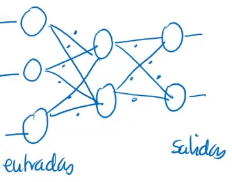
\includegraphics[scale=.82]{image-20210312102144206.png}}
\end{figure}
\vspace{-.5cm}
Es un \textbf{conjunto de neuronas conectadas entre sí} que se distribuyen en capas.

\textbf{Ventajas}:
\vspace{-.5cm}
\begin{itemize}

\item
  Son robustas ante el ruido.
\item
  Trabajan con datos complejos (difíciles de clasificar, como sensores)
\item
  Éxito en reconocimiento del habla y visión. Deep learning
\item
  Dan buenos resultados.
\end{itemize}

\textbf{Desventaja}: El aprendizaje es lento.

En las redes multicapa el cálculo del error se complica, hay varias
salidas y capas ocultas.

\subsection{Backpropagation o Retropropagación}

Se basa en:
$Error \sim \sum _{d \in D} \sum_{k \in outputs} (t_{kd}-o_{kd})^2$.
Para cada ejemplo:

\begin{enumerate}
\def\labelenumi{\arabic{enumi}.}

\item
  Se propaga desde la \textbf{entrada hasta la salida} (calcular la salida de la red)
\item
  \textbf{Propagación del error hacia atrás}: En las que están en la
  última capa es fácil, pero para las que están en las capas intermedias
  no tanto.

  \begin{enumerate}
  \def\labelenumii{\arabic{enumii}.}
  
  \item
    Se calcula el \textbf{error en la unidad de salida}:
    \(\delta_k \leftarrow\) \(o_k(1-o_k)(t_k-o_k)\) Este valor es el
    (t-o) de la variación delta, en este caso para una función sigmoide
    en vez de lineal
  \item
    \textbf{En las capas ocultas}: Se calcula con las unidades que están
    conectadas posteriormente,
    \(\delta_n \leftarrow o_n(1-o_n)\sum_{k \in output} w_{kn}\delta_k\)
  \end{enumerate}
\end{enumerate}

\subsection{Deep Learning}

Redes neuronales convolucionales. Se usan para procesado de imágenes.

\textbf{Puede recibir datos en crudo, no necesita que se los pasemos
como atributo valor}, lo que es una ventaja no hay que elegir los atributos
relevantes y organizar los datos. Recibe el grueso de los datos y los
va cogiendo por partes y agrupando, Convolution. Después se reduce la
resolución de la imagen, Pooling. Se repite el proceso hasta que tenemos
los datos para clasificar, extracción de características, y podemos
generar una red neuronal totalmente conectada, classification.

\begin{figure}[H]
	\ffigbox[\FBwidth]
	{\caption{Diagrama de Deep Learning}}
	{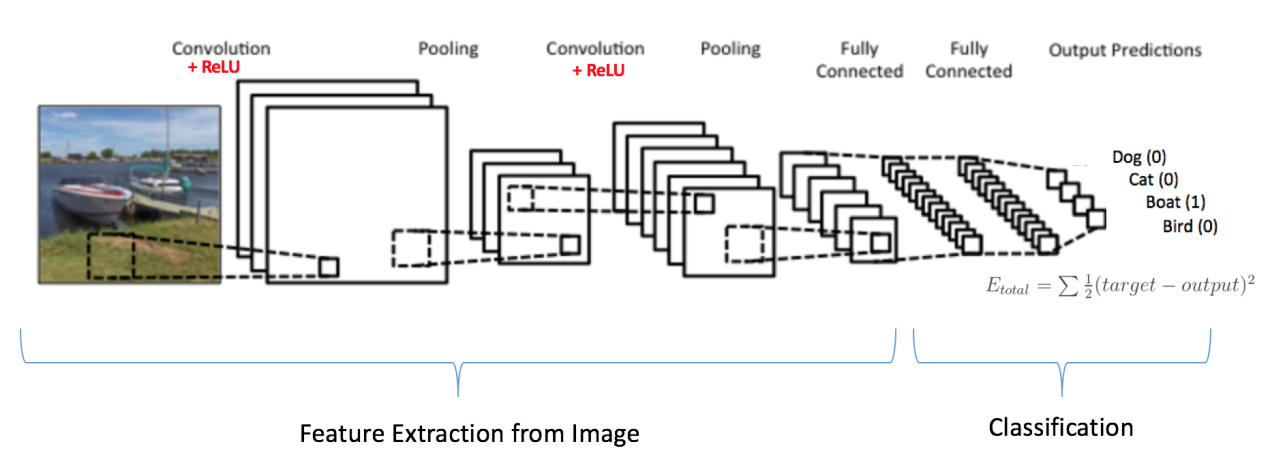
\includegraphics[scale=.3]{image-20210312111406573.png}}
\end{figure}

\section{Algoritmos genéticos}
\begin{figure}[H]
	\ffigbox[\FBwidth]
	{\caption{Diagrama Genético}}
	{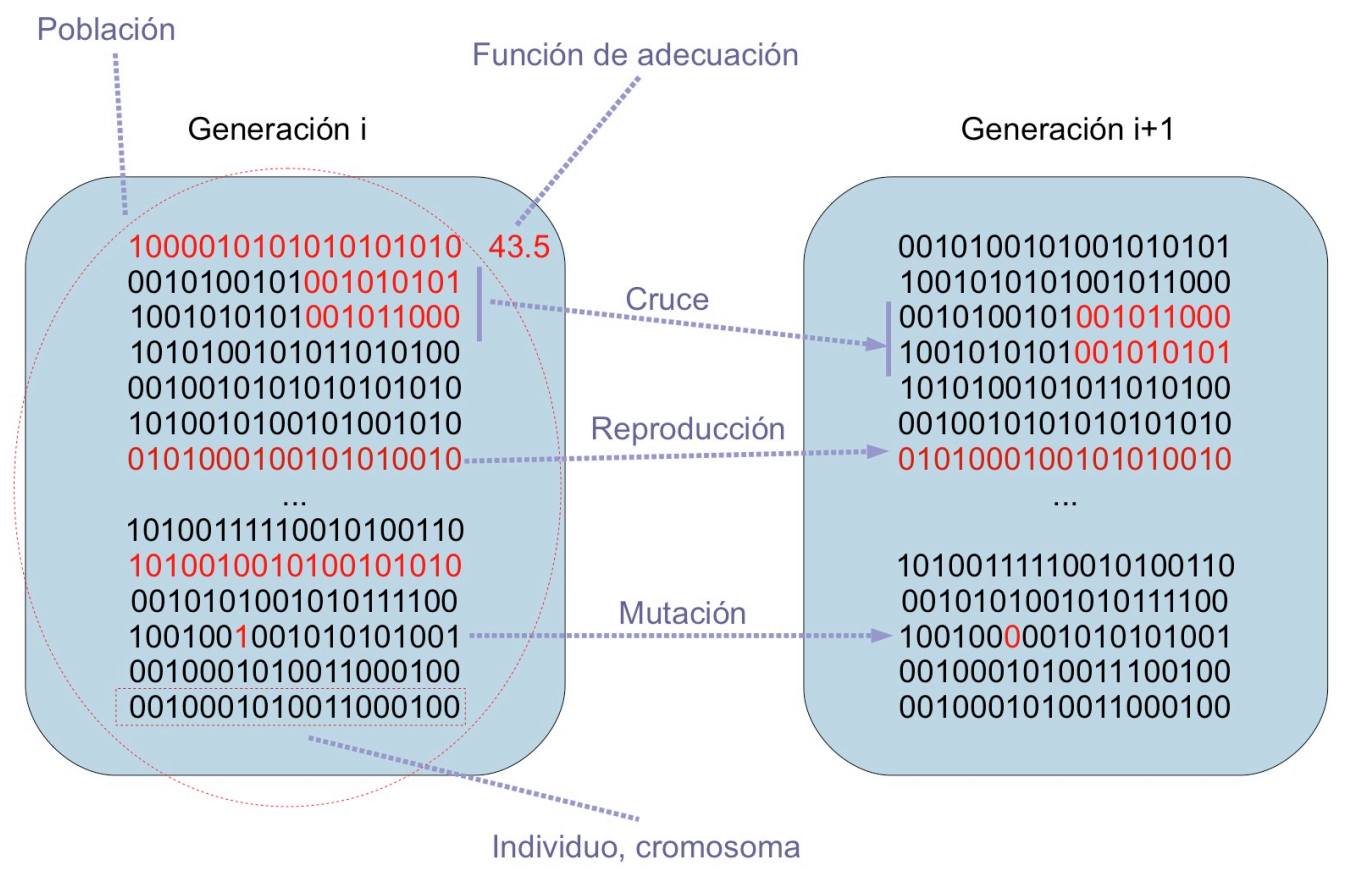
\includegraphics[scale=.4]{2021-03-19 11_26_59-otras-tecnicas.pdf - Foxit Reader.png}}
\end{figure}
Aprendizaje basado en evolución simulada, se mantiene una colección de soluciones, se evoluciona a través de generaciones por recombinación de las más adecuadas y eliminación de las menos adecuadas, y se termina cuando se obtiene una solución suficientemente adecuada.

\textbf{Son algoritmos de búsqueda local estocástica}, que las acciones tienen una probabilidad de ocurrir, son buenos para la optimización.

Hacen \textbf{búsqueda en el espacio de soluciones}, se usan cuando es fácil encontrar una solución, pero no la óptima. Funcionan por generaciones, en la que cada \textbf{generación} tiene una \textbf{población}, que está compuesta por p \textbf{individuos}, cada uno es una solución al problema.

\textbf{Factores clave:}
\begin{itemize}
  \item Elegir como representar los datos, se pueden utilizar cadenas de bits (llamado Genético) o alguna estructura de datos más compleja.
  \item Las operaciones para combinar soluciones y generar soluciones nuevas.
  \item La \textbf{función de adecuación (fitness)} que indica como de buena es una población, cuanto más es mejor. Transforma el genotipo (cadena de bits) en el fenotipo (significado de la cadena bits).
\end{itemize}
\pagebreak
\textbf{Proceso:}
\begin{figure}[H]
	\ffigbox[\FBwidth]
	{\caption{Algoritmo genético}}
	{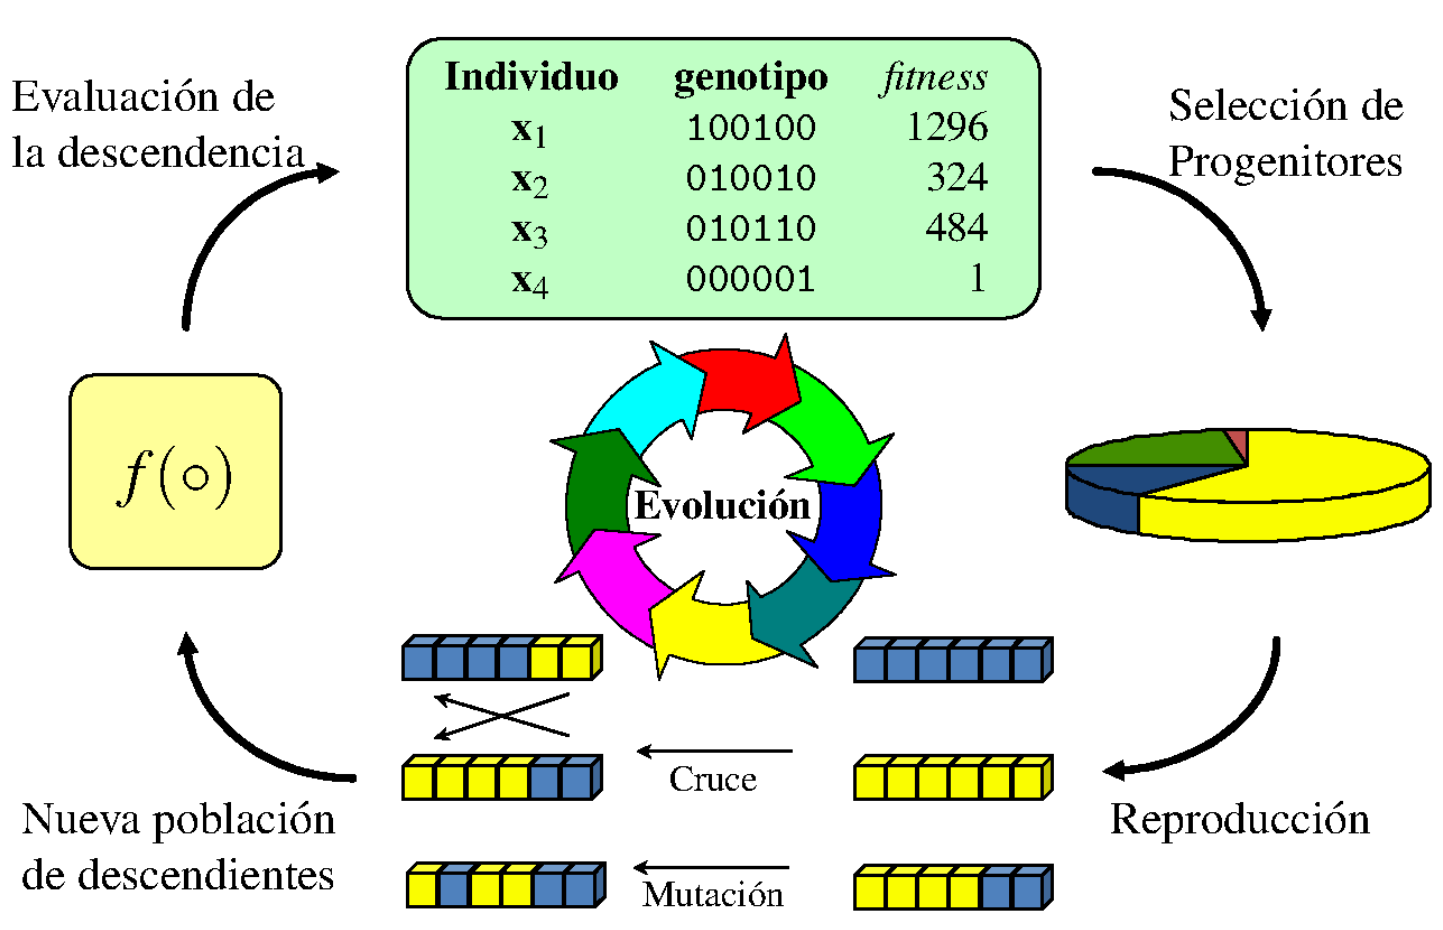
\includegraphics[scale=.3]{2021-03-19 11_42_34-otras-tecnicas.pdf - Foxit Reader.png}}
\end{figure}
\begin{enumerate}
  \item Se selecciona un conjunto de individuos de la población de soluciones. Se pueden elegir por Ruleta (por número aleatorio) o por Torneo (se coge un par de individuos y se escoge el mejor, dejando al otro fuera).
  \item A la nueva población se le realizan una serie de modificaciones como: reproducción, cruce, mutaciones y clone. Y quedan unos sobrevivientes, siempre tiene el mismo número de individuos.
  Cada operación tiene una probabilidad, por eso es búsqueda estocástica.
  \begin{description}
    \item[Cruce] Una parte de un par de individuos, mezcla de los progenitores.
    \item[Reproducción] Pasa a la nueva generación/población igual.
    \item[Mutación] Cambios muy pequeños, un solo bit.
  \end{description}
  \item Se evalúa la nueva población. Si es mejor pasa a ser la población base (generación), Si no se descarta y se intentan otras alternativas.
\end{enumerate}

\chapter{Tema 5: Técnicas Vagas y No Supervisadas}
\section{Aprendizaje basado en instancias (IBL)}
No genera modelo, lo que hace es que cuando recibe un dato nuevo busca algunos similares de los conocidos.
\begin{figure}[H]
	\ffigbox[\FBwidth]
	{\caption{Estrategia IBL}}
	{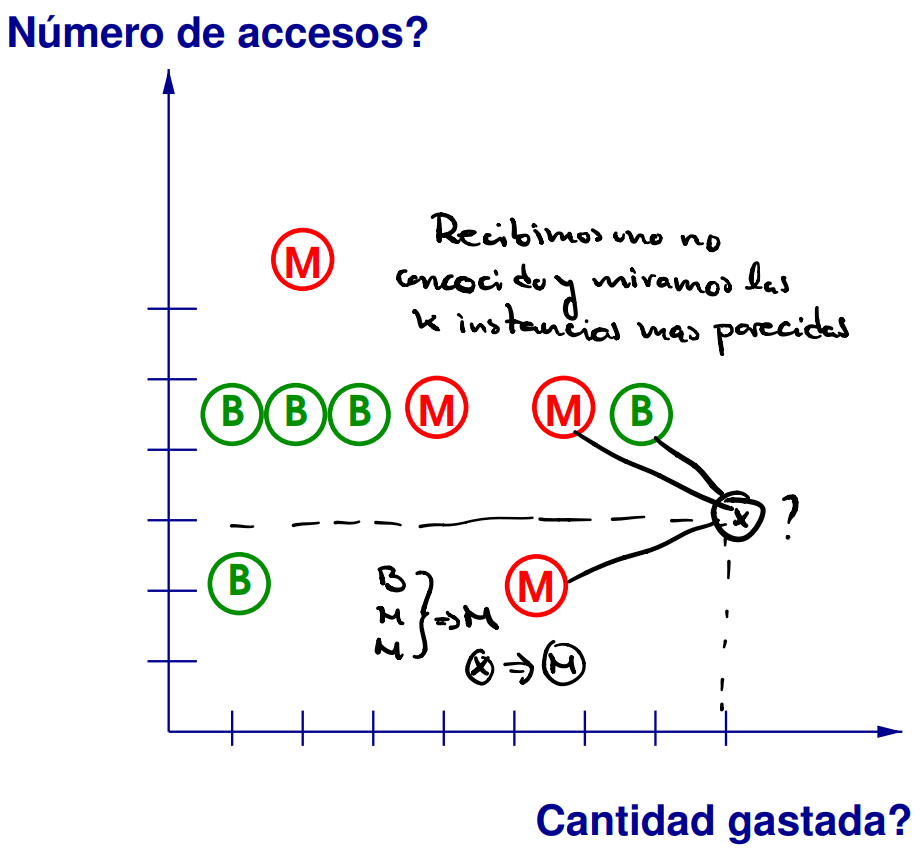
\includegraphics[scale=.3]{2021-03-19 12_05_34-Aprendizaje basado en instancias y no supervisados.pdf - Foxit Reader.png}}
\end{figure}
\textbf{Fases:}
\begin{enumerate}
  \item \textbf{Entrenamiento:} Almacenamiento de todo el conjunto de datos disponibles.
  \item \textbf{Generalización:} Cuando recibe un nuevo dato, se cogen un conjunto de datos similares, que son utilizados para clasificar el nuevo dato. Todo el cómputo se realiza en tiempo de clasificación, Aprendizaje Perezoso.
\end{enumerate}
Para definir similitud, se utilizan medidas de distancia (más cercano, más similares).

El algoritmo recibe como entrada k, que indica el número de vecinos más cercanos que se van a considerar (K-NN, K-Nearest Neighbors). 

\subsection{K-Nearest Neighbors}
Las instancias corresponden a puntos en un espacio de dimensión n (n atributos) y los vecinos más cercanos se calculan con la distancia euclídea ($d\left( \vec{x},\vec{z}\right)   = \sqrt {\sum _{i=1}^{n}  \left( x_{i}-z_{i}\right)^2 }$).

Si los atributos tienen diferentes rangos, se normalizan, y si son valores simbólicos, se define el valor por posible valor.
\subsection{Función Objetivo}
Dada una instancia x y sus k vecinos, nos indica cuál es la clase. Dependiendo del tipo de valores se usan distintos métodos:
\begin{description}
  \item[Caso discreto (clasificación)] Valor más común de entre los k vecinos más cercanos.
  \begin{figure}[H]
    \begin{eqnarray}
      \hat{f}(\vec{x}) &=& \arg\max _{c \in C} \sum^k_{i=1} \delta(c,f(\vec{z^i})) \\
      \hat{f}(\vec{x}) &=& \arg\max _{c \in C} \sum^k_{i=1} w_i \times \delta(c,f(\vec{z^i}))
    \end{eqnarray}
    \captionsetup{justification=centering}
    \caption{Función objetivo K-Nearest: Clasificación}
  \end{figure} 
  \item[Caso continuo (regresión)] Valor medio de entre los k vecinos. 
  \begin{figure}[H]
    \begin{eqnarray}
      \hat{f}(\vec{x}) &=& \frac{\sum^k_{i=1} f(\vec{z^i})}{k}\\
      \hat{f}(\vec{x}) &=& \frac{\sum^k_{i=1} w_i f(\vec{z^i})}{\sum^k_{i=1} w_i}
    \end{eqnarray}
    \captionsetup{justification=centering}
    \caption{Función objetivo K-Nearest: Regresión}
  \end{figure}
\end{description}
También se puede ponderar la importancia de cada vecino en el valor de la función objetivo, en función de su distancia. Donde $w_i = \frac{1}{d(\vec{x},\vec{z^i})^2}$.

\subsection{Selección de los K vecinos}
El parámetro k identifica cuantos vecinos se utilizan para la decisión, su valor es el que mejor resultados aporta, no hay una regla que siempre funcione. Las regiones que se forman con 1-NN se denominan regiones de Voronoi.

\subsection{Medidas de distancia}
\begin{description}
  \item[Distancia de Hamming (atributos no numéricos)] $\left(x_{m}-z_{m}\right)=\left\{\begin{array}{ll}0 & \text { si } x_{m}=z_{m} \\ 1 & \text { si } x_{m} \neq z_{m}\end{array}\right.$
  \item[Manhattan] $d(\vec{x}, \vec{z})=\sum_{m=1}^{n}\left|x_{m}-z_{m}\right|$
  \item[Minkowski] $d(\vec{x}, \vec{z})=\left(\sum_{m=1}^{n}\left|x_{m}-z_{m}\right|^{k}\right)^{\frac{1}{k}}$
\end{description}
\pagebreak
\subsection{Propiedades}
\begin{itemize}
  \item Las instancias son puntos de un espacio n dimensional, donde n es el número de atributos.

  \item No hay muchos atributos por instancias, 20 aprox.

  \item Hay muchos datos de entrenamiento.

\end{itemize}

\subsubsection{Ventajas}
\begin{itemize}
  \item Simple e intuitivo.

  \item Fácil de usar.

  \item Funciona bien cuando la función objetivo es muy compleja.

  \item El entrenamiento es muy rápido.

  \item Efectivo si hay muchos ejemplos. Consistente asintóticamente: Con infinitos ejemplos y un k suficientemente grande, es capaz de aproximarse al mejor clasificador (Bayes óptimo).

\end{itemize}
\subsubsection{Problemas y sus soluciones}
\begin{itemize}
  \item Muy \textbf{sensible a atributos irrelevantes}
  \begin{itemize}
    \item \textbf{Selección de atributos:} Determinar qué características son las interesantes, y eliminar las restantes. Se pueden utilizar técnicas wrapper, que busca en el espacio de atributos, métodos estadísticos, algoritmos genéticos, etc.
    \item \textbf{Ponderación de atributos:} Es menos radical que eliminar atributos y consiste en dar el peso que minimice el error a los distintos atributos a la hora de seleccionar vecinos por distancia.
  \end{itemize}
 
  \item \textbf{Coste de clasificación alto (tiempo)}, no tarda en entrenar, pero cuando clasifica compara todos los ejemplos
  \begin{itemize}
    \item \textbf{Indexación:} Organizar el conjunto de instancias
    \begin{itemize}
      \item \textbf{Árboles KD (k dimensional):} Particionar el espacio en regiones marcadas por las instancias que tenemos, en el que cada rama va reduciendo el espacio. Alterna entre dimensiones.
      
      \begin{figure}[H]
        \ffigbox[\FBwidth]
        {\caption{Ejemplo Árbol KD}}
        {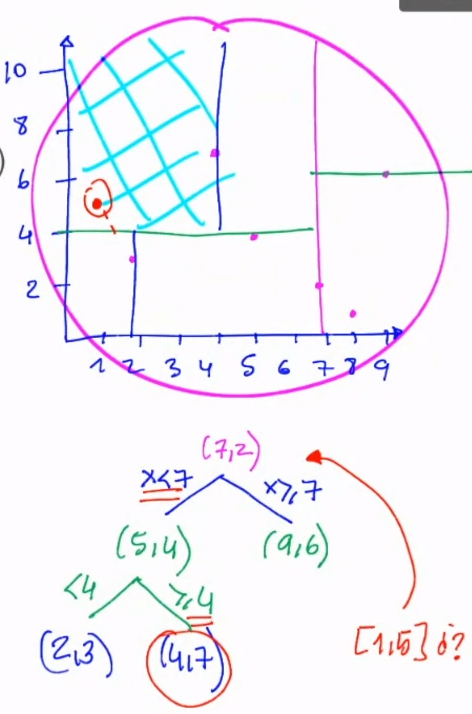
\includegraphics[scale=.7]{2021-03-19 14_58_39-AA IBL y no supervisados I.mkv.png}}
      \end{figure}

      \item \textbf{Agrupación o clustering:} Que es de aprendizaje no supervisado.
    \end{itemize}
  \end{itemize}
  \item \textbf{Almacenamiento (memoria) de todos los ejemplos}
  \begin{itemize}
    \item \textbf{Selección de instancias:} Elegir un grupo reducido de instancias (prototipos, ejemplos representativos) que mantengan la misma información que el conjunto total. Se puede hacer de manera incremental, desde el conjunto vacío e ir añadiendo, o decremental, desde el conjunto completo y eliminando. Se sigue un criterio para sacar o meter una instancia en el conjunto, que siga clasificando correctamente o se reduce las que clasifica mal.
    \item \textbf{Reemplazo de instancias:} Calcular prototipos a partir del conjunto de entrenamiento, y esos prototipos podrían sustituirse por los ejemplos que lo han generado. Se pueden generar con técnicas de clustering.
  \end{itemize}

\end{itemize}
\subsection{Otros métodos}
\subsubsection{Locally Weighted Regression}
En vez de devolver la media de la clase de los k vecinos, se crea un modelo lineal de forma local en zonas del espacio. Por cada consulta se obtienen los k vecinos y se crea el modelo de regresión lineal.

Se podría aplicar cualquier otro método de aproximación, como las redes neuronales.
\subsubsection{Case Based Reasoning}
Los ejemplos no son de la forma atributo-valor, sino que se representan con cualquier estructura de datos, como pueden ser imágenes, documentos, planos, etc. Consigue adaptar los datos de otros problemas al actual, viendo cómo se han resuelto problemas previos.

\section{Aprendizaje no supervisado}
No conocemos la clase, solo tenemos atributos en los ejemplos.

Lo que se hace es ver que instancias son parecidas y se crean grupos de instancias similares. También se utiliza para reducir el número de instancias y quedarnos con el más representativo del grupo.

\subsection{Posibles objetivos}
\begin{itemize}
  \item \textbf{Agrupación:} Dado un conjunto de ejemplos sin etiquetar, agruparlos según algún criterio.
  \item \textbf{Indexación:} Dado un conjunto de ejemplos, facilitar su acceso organizándolos.
  \item \textbf{Asociación:} Dados unos datos, establecer relaciones y/o asociaciones entre datos.
  \item \textbf{Generación de jerarquías:} Dados unos datos en un mismo nivel, generar jerarquías en dichos datos.
  \item \textbf{Reducción de dimensionalidad:} Dados unos datos, reducir la dimensión o número de atributos que caracterizan los datos.
  \item \textbf{Visualización:} Dados unos datos con representación compleja, permitir su visualización.
\end{itemize}

\subsection{Agrupación}
El objetivo es dado un conjunto de ejemplos sin etiquetar, agruparlos siguiendo algún criterio predefinido. Usaremos la técnica k-medias.
Ese criterio suele venir por:
\begin{itemize}
  \item \textbf{Aprendizaje paramétrico:} Parámetros asumidos, se asume que los datos siguen una distribución.
  \item \textbf{Aprendizaje no paramétrico:} Necesitamos alguna medida de distancia para ver cuáles se parecen más entre ellos. Se basa en agrupar las instancias por similitud; a menor distancia, mayor similitud. 

  Se puede utilizar Distancia euclídea (la más usada) $d\left( \vec{x},\vec{z}\right)   = \sqrt {\sum _{i=1}^{n}  \left( x_{i}-z_{i}\right)^2 }$, euclídea ponderada $d\left( \vec{x},\vec{z},\vec{w}\right)   = \sqrt {\sum _{i=1}^{n} w_i \left( x_{i}-z_{i}\right)^2 }$, etc.

  \textbf{Tipos de técnicas:}
  \begin{itemize}
    \item Técnicas de particionamiento (como k-medias).
    
    La salida es un conjunto de clases/grupos de instancias.

    \item Técnicas Aglomerativos (jerárquica).
    
    La salida es una jerarquía de clases, en cada clase hay instancias, pero hay clases de clases con mayor importancia.
  \end{itemize}
\end{itemize}

\subsubsection{k-medias o Algoritmo de Lloyd}

Realiza una discretización o particionamiento del espacio.

Genera regiones de Voronoi y nos proporciona un representante de la región, se definen mediante una medida de distancia y un conjunto de ejemplos representativos.

\textbf{Objetivo:} Generar el conjunto de prototipos/centroides que minimice una determinada medida de error o distorsión.


\textbf{Algoritmo de Lloyd Generalizado (T, k):} Conjunto de entrenamiento T y k número de grupos/clases. Los prototipos se representan con $\mu$.

\begin{enumerate}
  \item Comenzar con un conjunto inicial de k prototipos $C_1 = \{\vec{\mu_1}, ..., \vec{\mu_k} \}$.
  \item Dado un conjunto de prototipos, $C_m$, ejecutar la Iteración de Lloyd para generar el siguiente conjunto de prototipos, $C_{m+1}$. Los prototipos varían entre conjuntos, se van centrando.
  
  \textbf{Iteración de Lloyd ($C_m$, T, k):} $C_m$ Conjunto prototipo, T Conjunto de entrenamiento y k número de grupos. Crea regiones y recalcula centroide.
  \begin{enumerate}
    \item Dado un conjunto de prototipos $C_m = \{\vec{\mu_1}, ..., \vec{\mu_k} \}$, partir el conjunto de entrada T en k particiones $R_i, ..., R_k$ usando la siguiente condición: Los ejemplos pertenecen a la región del prototipo más cercano, y solo de ese. (Si se genera una partición vacía, utiliza alguna estrategia para tratar el caso)
    
    $$R_i = \{ \vec{x} \in T: d(\vec{x}, \vec{\mu_i}) \leq d(\vec{x}, \vec{\mu_j}); \forall j \neq i \}$$
    
    \item Recalcular los centroides de cada partición, pasa a ser el punto medio de la región, y actualiza el conjunto de prototipos con esos centroides.
    $$centroide(R_i) = \frac{1}{|R_i|} \sum_{\vec{x} \in R_i} \vec{x}$$
  \end{enumerate}
  \item Calcular la distorsión para el nuevo conjunto, $C_{m+1}$, midiendo como de cerca están las instancias $x_i$ del prototipo $\mu_j$.
  $$D = \sum^{|T|}_{i=1} d( \vec{x_i}, \vec{\mu_j})^2$$
  $$C_{m+1} = \{\vec{\mu_i}|\vec{\mu_i} = centroide(R_i) \}$$
  \item Si el decremento de la distorsión entre dos interacciones no supera un umbral (bastante bajo), parar. Si no ir al paso 2. 
\end{enumerate}

\textbf{Ejemplo:}

\begin{figure}[H]
  \ffigbox[\FBwidth]
  {\caption{k-medias I}}
  {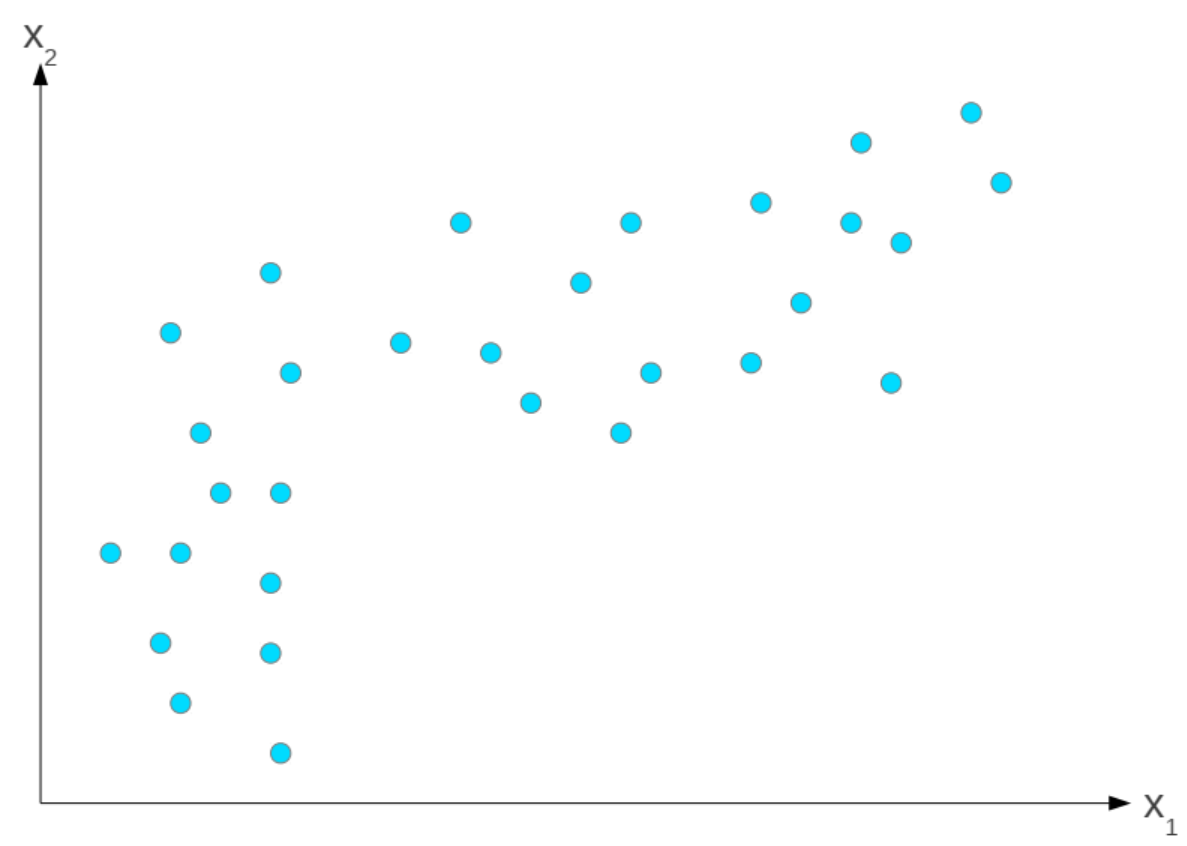
\includegraphics[scale=.2]{2021-03-26 09_37_22-Aprendizaje basado en instancias y no supervisados.pdf - Foxit Reader.png}
  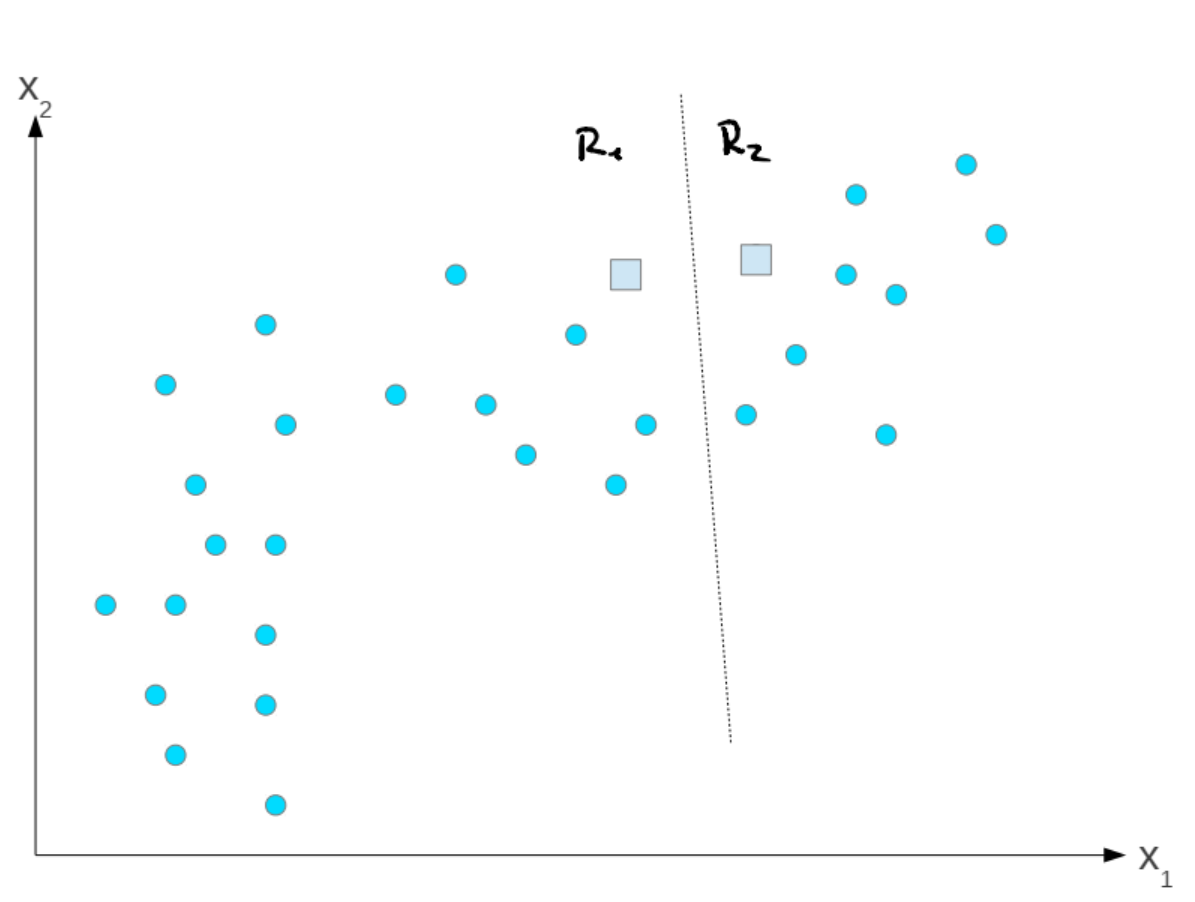
\includegraphics[scale=.2]{2021-03-26 09_38_09-Aprendizaje basado en instancias y no supervisados.pdf - Foxit Reader.png}}
\end{figure}

\begin{figure}[H]
  \ffigbox[\FBwidth]
  {\caption{k-medias II}}
  {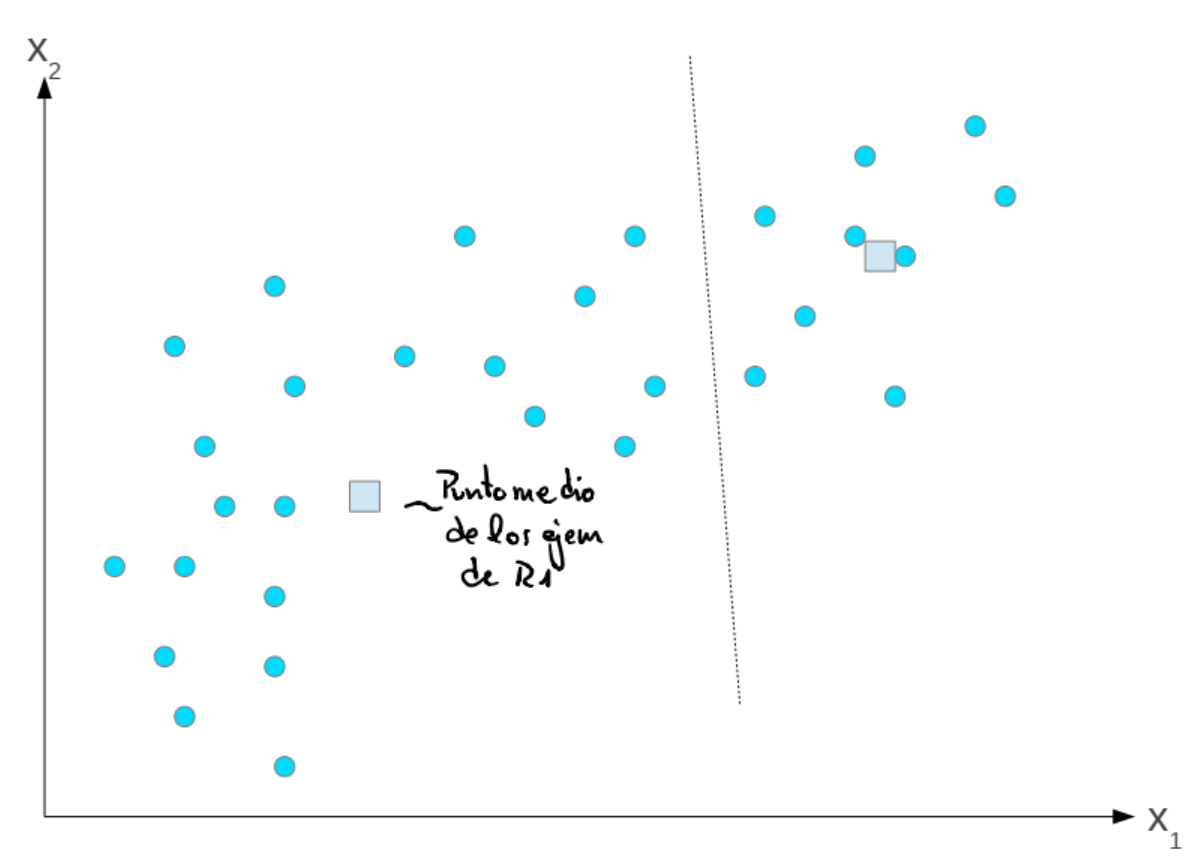
\includegraphics[scale=.2]{2021-03-26 09_39_23-Aprendizaje basado en instancias y no supervisados.pdf - Foxit Reader.png}
  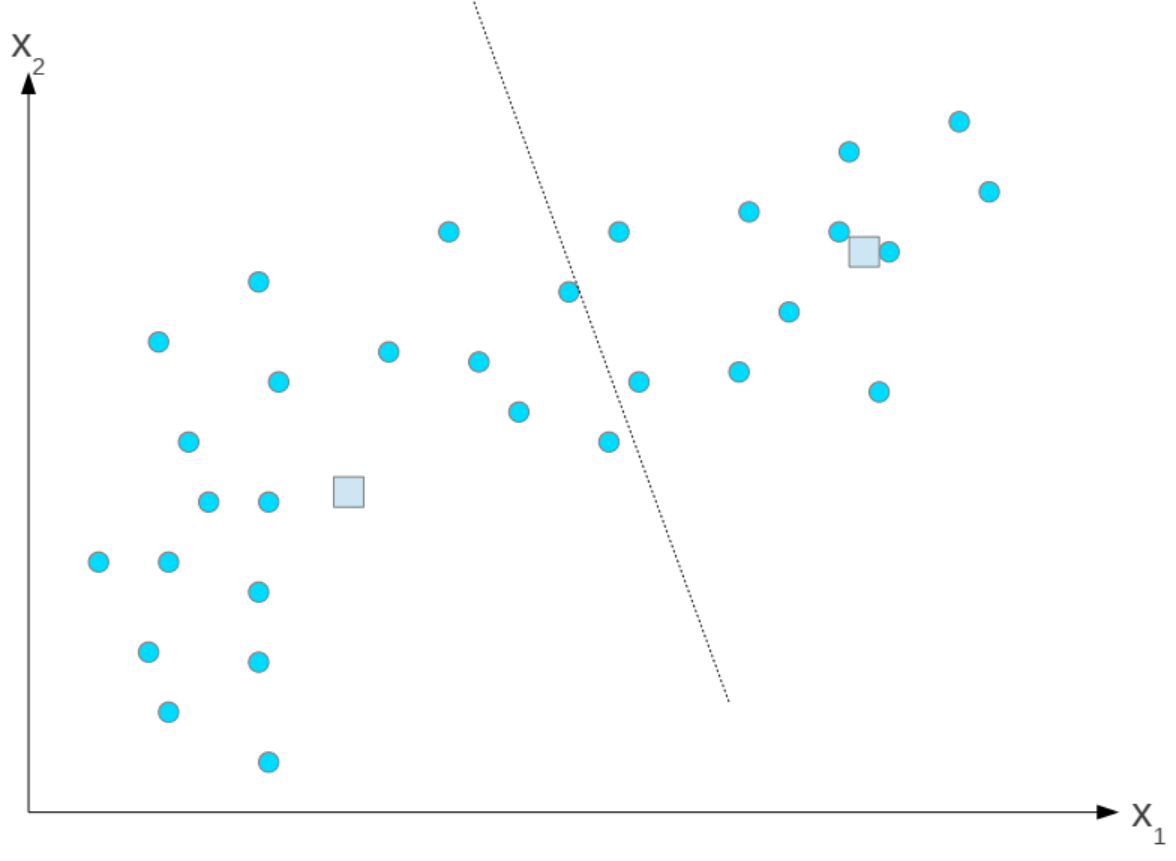
\includegraphics[scale=.2]{2021-03-26 09_39_55-Aprendizaje basado en instancias y no supervisados.pdf - Foxit Reader.png}}
\end{figure}

\textbf{Algunas consideraciones:}
\begin{itemize}
  \item Atributos con diferentes rangos es imprescindible normalizarlos.
  \item Atributos simbólicos: Utilizamos Distancia de Hamming. 
\end{itemize}

\textbf{Parámetros de k-medias:}

Nos indica el número de clases a considerar y nos sirve para la selección de semillas.

Selección de semillas:
\begin{itemize}
  \item ejecutar varias veces y quedarse con la mejor partición.
  \item otra alternativa es utilizar K-MEANS++ (que es una selección más inteligente)
\end{itemize}

Selección de k automáticamente:
\begin{itemize}
  \item Se puede probar con distintos k y quedarse con el que los conjuntos tengan menos distorsión.
  \item Otro método es G-MEANS.
\end{itemize}

\subsubsection{Métodos Aglomerativos}

Consisten en generar unos árboles denominados dendrogramas.

\textbf{Clustering jerárquico:} No solo se generan grupos, sino también una jerarquía entre ellos.

\textbf{Búsqueda hacia arriba:} 
\begin{enumerate}
  \item Inicialmente, cada ejemplo representa una clase.
  \item Se repite N-1 veces (siendo N el número de ejemplos):
  \begin{enumerate}
    \item Se calcula la similitud entre todo par de ejemplos.
    \item Se agrupan los dos más cercanos.
    \item Se sustituyen los dos nodos por su representante/centroide/prototipo.
  \end{enumerate}
\end{enumerate}

\textbf{Ejemplo:}

\begin{figure}[H]
  \ffigbox[\FBwidth]
  {\caption{Clustering jerárquico I}}
  {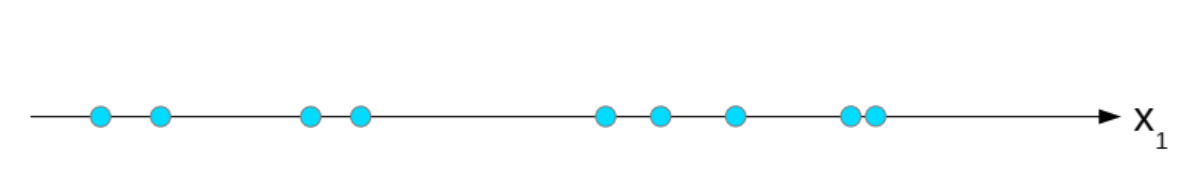
\includegraphics[scale=.2]{2021-03-26 10_12_33-Aprendizaje basado en instancias y no supervisados.pdf - Foxit Reader.png}
  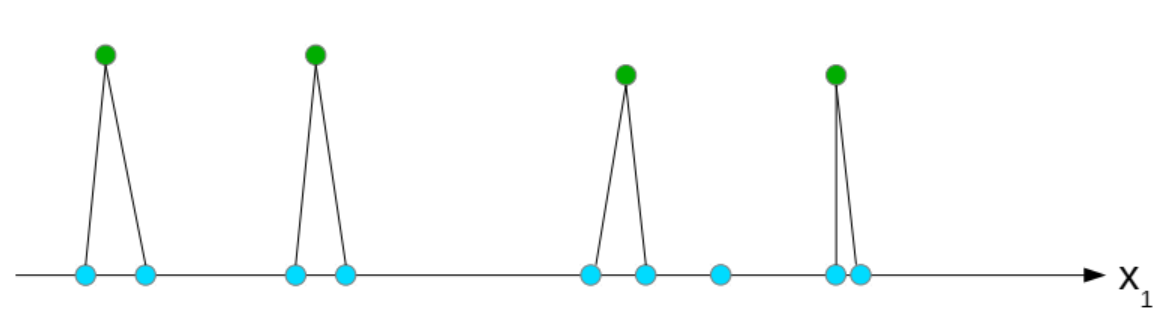
\includegraphics[scale=.2]{2021-03-26 10_13_31-Aprendizaje basado en instancias y no supervisados.pdf - Foxit Reader.png}}
\end{figure}

\begin{figure}[H]
  \ffigbox[\FBwidth]
  {\caption{Clustering jerárquico II}}
  {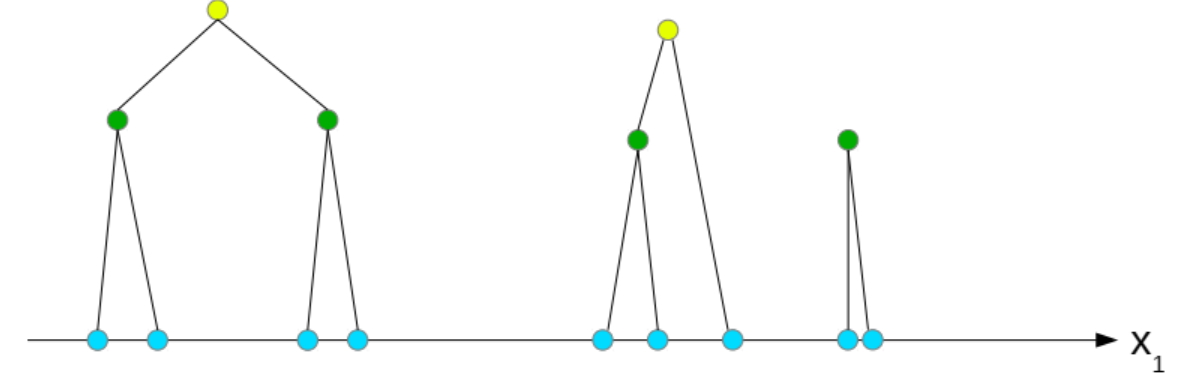
\includegraphics[scale=.2]{2021-03-26 10_13_56-Aprendizaje basado en instancias y no supervisados.pdf - Foxit Reader.png}
  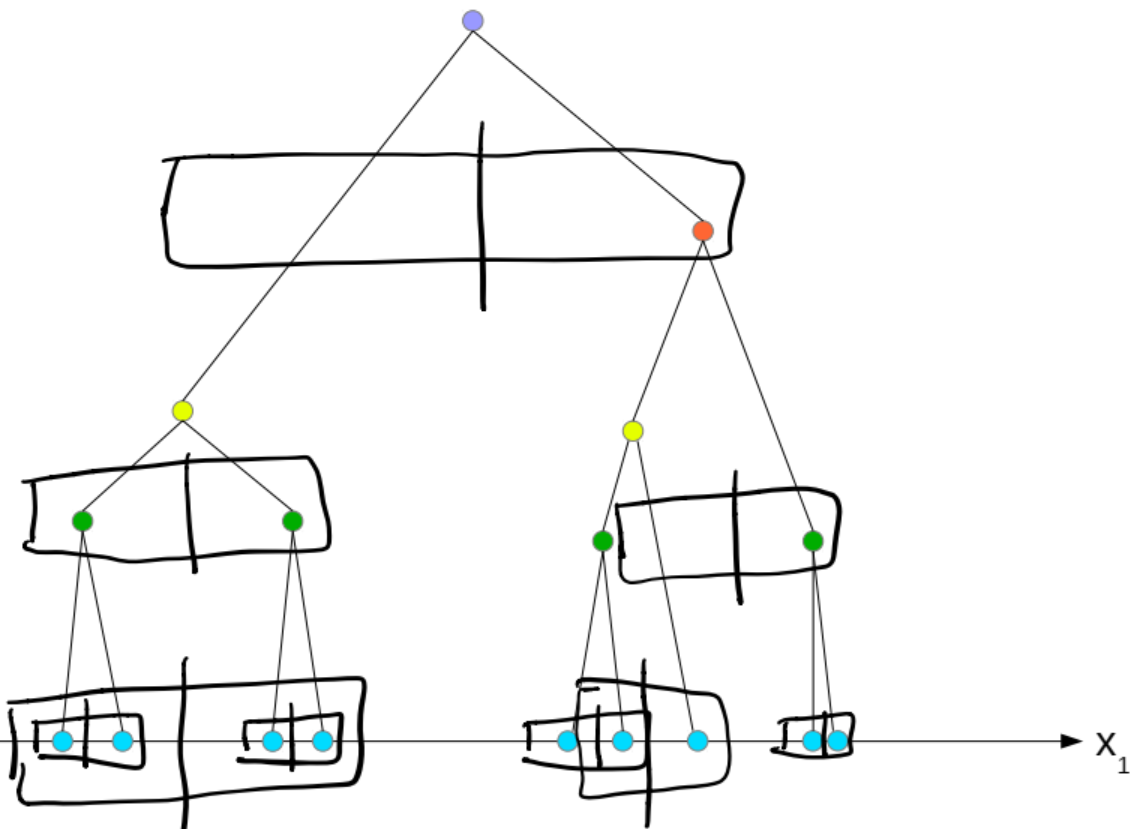
\includegraphics[scale=.2]{2021-03-26 10_14_24-Aprendizaje basado en instancias y no supervisados.pdf - Foxit Reader.png}}
\end{figure}

\pagebreak

\subsubsection{Distancia entre clústeres}

Distintas definiciones:
\begin{itemize}
  \item Mínima entre las instancias de los clústeres. $d_{min}(C_i, C_j) = \min_{\vec{x} \in C_i, \vec{y} \in C_j} d(\vec{x}, \vec{y})$
  \item Máxima. $d_{max}(C_i, C_j) = \max_{\vec{x} \in C_i, \vec{y} \in C_j} d(\vec{x}, \vec{y})$
  \item Media. $d_{media}(C_i, C_j) = \frac{1}{|C_i||C_j|} \sum_{\vec{x} \in C_i, \vec{y} \in C_j} d(\vec{x}, \vec{y})$
  \item Como distancia entre sus centroides. $d_{centro}(C_i, C_j) = d(\vec{\mu_i}, \vec{\mu_j})$
\end{itemize}

\section{Aprendizaje semi-supervisado}

En algunos dominios etiquetar es pesado (páginas web, imágenes). La solución es etiquetar unas pocas instancias.

\subsection{co-training [Blum and Mitchell, 1998]}

Se tienen dos conjuntos de datos independientes con diferentes atributos, que entrenan clasificadores independientes, y se etiquetan las demás instancias con la clase que diga el clasificador que tenga más confianza y se repite el proceso.

\subsection{CO-EM}

Entrena con las clasificadas, clasifica el resto y el resultado se añade al conjunto de entrenamiento.

Realiza en bucle: Clasificar las instancias no etiquetadas y reconstruir el clasificador.

Es aprendizaje supervisado con las instancias etiquetadas.

\chapter{Tema 6: Conjuntos de clasificadores y Reglas de asociación}
\section{Conjuntos de clasificadores - Emsembles}
Se emplea en aprendizaje supervisado, la mayoría se pueden utilizar tanto en Clasificación como en Regresión, pero hay algunos más específicos.

Se tiene un grupo de clasificadores cuyas decisiones individuales se combinan de alguna manera. A menudo son mucho más precisos que cualquiera de los clasificadores individuales.

Los clasificadores individuales deben ser diversos (errores no correlados) y precisos (al menos mejor que una clasificación aleatoria).

Razones por las que se pueden encontrar buenos conjuntos:
\begin{itemize}
  \item \textbf{Estadística:} Si construimos muchos modelos que no tengan mucha precisión, combinando los modelos estadísticamente se reduce el error.
  \item \textbf{Computacional:} Como cada hipótesis se construye de manera diferente, combinar varias búsquedas locales, nos permite encontrar un modelo final más preciso sin la necesidad de explorar todo el espacio de hipótesis.
  \item \textbf{Representacional:} Es posible que combinando distintas hipótesis (en la que alguna puede estar en un espacio de hipótesis que no contenga a la función) lleguemos a poder representar una mejor aproximación a la función real.
\end{itemize}

Métodos de construcción de conjuntos
\begin{itemize}
  \item Manipulación de las instancias del conjunto de entrenamiento
  \begin{itemize}
    \item Bagging
    \item Comités de validación cruzada
    \item AdaBoost (Boosting)
  \end{itemize}
  \item Manipulación de los atributos (utilizar atributos distintos en los clasificadores)
  \begin{itemize}
    \item Random forests
  \end{itemize}
  \item Manipulación de las salidas/clases
  \begin{itemize}
    \item Error correcting output coding - ECOC
  \end{itemize}
  \item Meta-Aprendizaje
  \begin{itemize}
    \item Stacking
  \end{itemize}
\end{itemize}

\subsection{Bagging - Boostrap aggregating [Breiman, 1996]}
Construir distintos conjuntos de entrenamientos, generar los clasificadores y la salida será lo que diga la mayoría de los clasificadores.

Generan muestras de m instancias del conjunto de entrenamiento, donde cada muestra se genera haciendo selección aleatoria con remplazo (una instancia se puede coger en varios conjuntos) Se genera un clasificador con cada muestra.

Los clasificadores se pueden generar en paralelo, y se combinan las decisiones de los clasificadores por voto mayoritario.

\begin{figure}[H]
  \ffigbox[\FBwidth]
  {\caption{Bagging}}
  {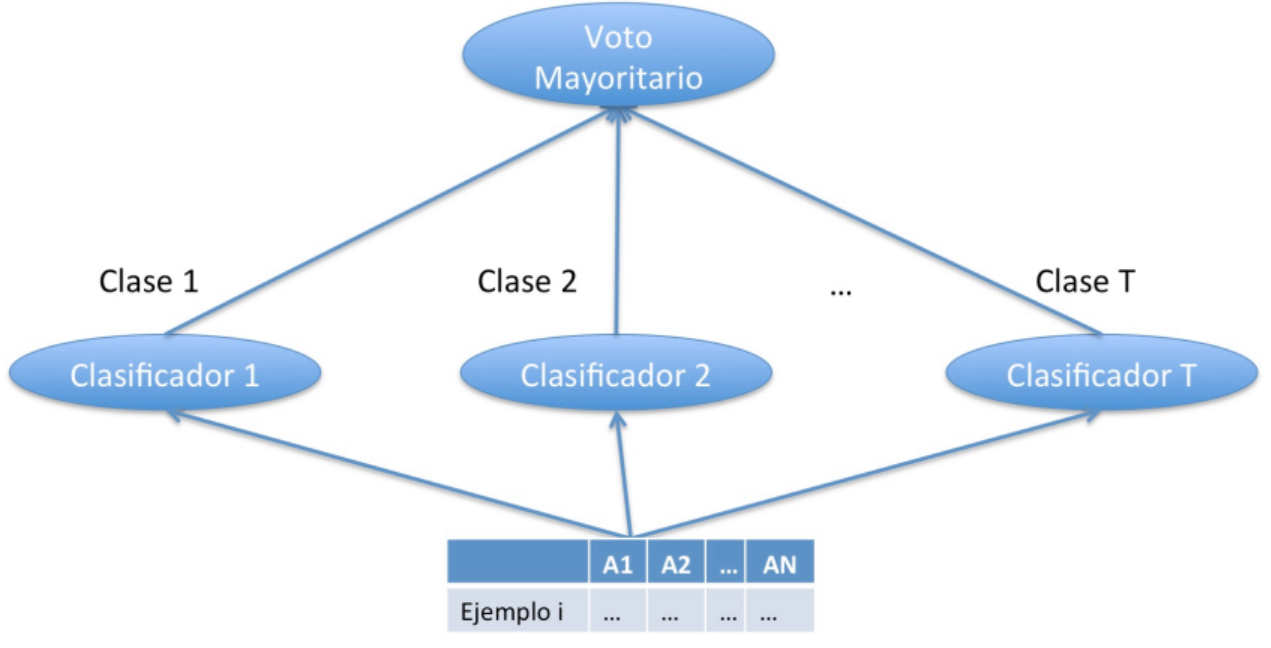
\includegraphics[scale=.3]{2021-04-09 23_26_39-Settings.png}}
\end{figure}

\subsubsection{Algoritmo de Bagging}
\textbf{Procedimiento Bagging (E, B, N)}, donde E es el conjunto de entrenamiento, B el algoritmo de aprendizaje y N el número de clasificadores que se generan (copias de E).

Para $i = 1$ hasta N:

\hspace{6mm} $E' =$ muestra de $E$ (selección aleatoria con reemplazo).

\hspace{6mm} $C_i = B(E')$ (crea un nuevo clasificador a partir de $E'$).

Devolver clasificadores $C_i$.

\subsection{Comités de validación cruzada}
Se construyen conjuntos de entrenamiento de forma similar a validación cruzada (básicamente igual, pero cada uno de los clasificadores que se utilizaría para estimar el error es lo que se busca):
\begin{itemize}
  \item Se dividen los ejemplos de entrenamiento en k conjuntos disjuntos.
  \item Se crean k conjuntos de entrenamiento en el que en cada uno se deja fuera uno de los conjuntos disjuntos.
\end{itemize}

\subsection{Boosting [Shapire, 1990]}
La idea es ir construyendo un clasificador (incremental) que basándose en lo que ha fallado previamente vaya mejorando, se especializan los clasificadores en ejemplos mal clasificados.

Se utiliza principalmente en clasificación binaria (+1 -1). Mejora la precisión de clasificadores débiles, como puede ser OneR.

El algoritmo de boosting más utilizado es AdaBoost - Adaptative Boosting.

Los clasificadores se generan de manera secuencial y se combina la decisión de los clasificadores por voto ponderado.
\subsubsection{Algoritmo de Boosting}
\begin{figure}[H]
  \ffigbox[\FBwidth]
  {\caption{Boosting}}
  {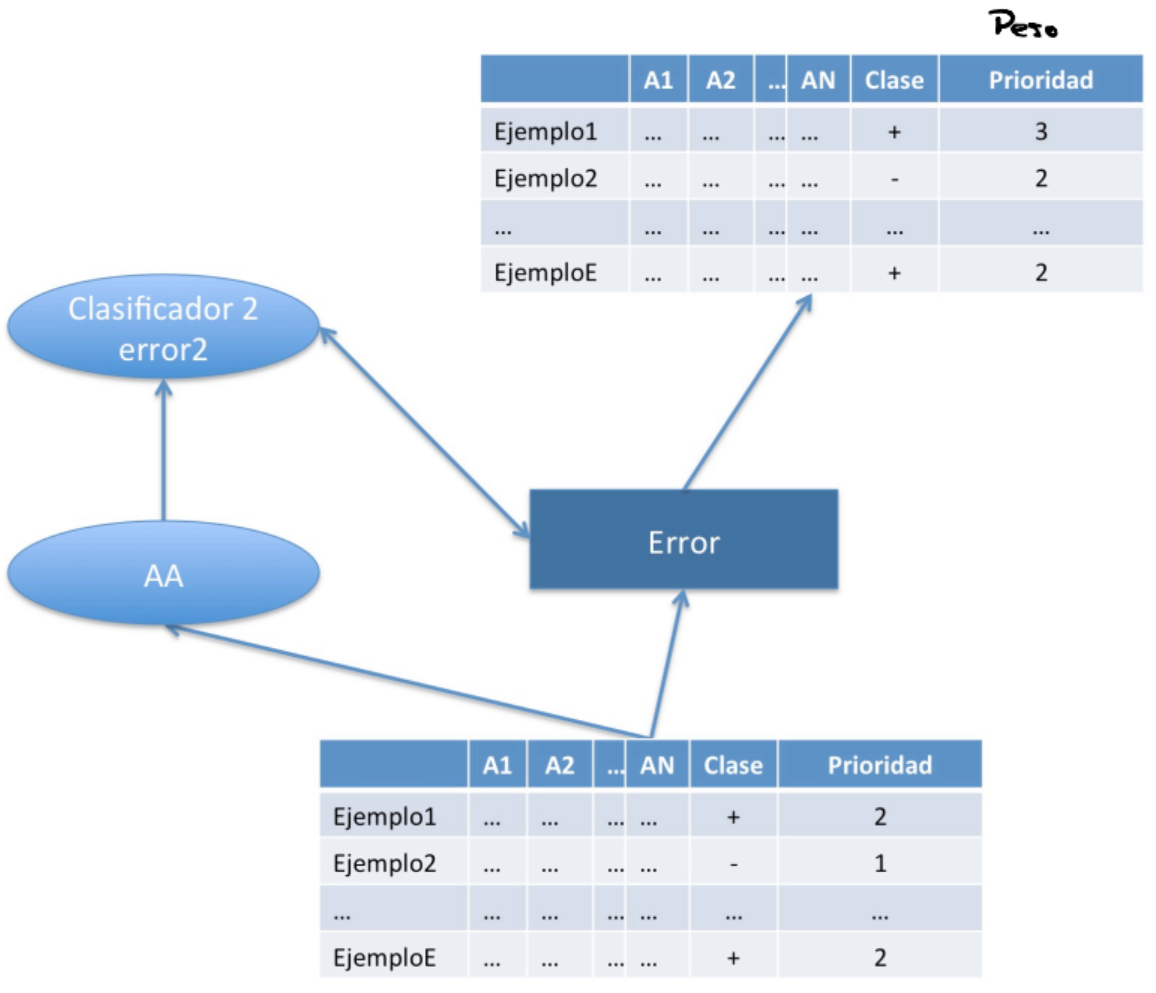
\includegraphics[scale=.25]{2021-04-10 00_10_42-ensembles-reglasAsociacion.pdf - Foxit Reader.png}}
\end{figure}

Se tienen unas instancias con unos pesos, se utiliza un algoritmo de aprendizaje que genera un modelo, se evalúan las instancias y según las mal clasificadas se recalculan los pesos de las instancias (que lo solucionaran los futuros clasificadores)

\textbf{Procedimiento AdaBoostM1(E, B, T)}, donde E es el conjunto de entrenamiento E, B el algoritmo de aprendizaje base y T el número de iteraciones.

Inicializar pesos: $w(x_i) = \frac 1 n$. Inicialmente todas las instancias (x) tienen el mismo peso.

Para $t = 1$ hasta $T$:
\begin{itemize}
  \item Normalizar pesos $w(x_i)$ (suman todas 1 en total)
  \item $C_t = B(E_t)$ Se construye un clasificador con el conjunto de entrenamiento con pesos.
  \item \textbf{Error por instancia:} $ierror(x_i)$ (0 si bien clasificado, 1 si mal clasificado)
  \item \textbf{Error del clasificador:} $error_{C_t} = \frac {\sum_i w(x_i)\cdot ierror(x_i)} {\sum_i w(x_i)}$ Medida ponderada, para tener en cuenta los pesos de las instancias y poder darles luego más importancia.
  \item \textbf{Peso del clasificador:} $peso_{C_t} = ln \left( \frac{1-error_{C_t}}{error_{C_t}} \right)$ Da más peso a los clasificados que cometen menos error (son más precisos)
  \item \textbf{Actualización de pesos:} $w(x_i) = w(x_i) \times e^{(peso_{C_t} \times ierror(x_i))}$ Da más peso a las instancias predichas incorrectamente. De esta manera se trata de que se llegue a clasificar bien (se va especializando)
\end{itemize}
Devolver clasificador C* donde cada clasificador se pondera por su peso.

De esta manera tenemos T clasificadores, a los que pasaremos instancias y tendremos en cuenta el peso del clasificador (ponderar el resultado) para elegir la clase final.

\subsection{Manipulación de atributos}
Se generan distintos clasificadores con distintos subconjuntos de atributos.

Problemas cuando eliminar atributos provoca un mal comportamiento de los clasificadores.

\subsection{Bosques aleatorios (Random Forests) [Breiman, 2001]}
Por un lado, se modifican instancias y por otros atributos.

\textbf{Aprendizaje:} Se construyen k árboles de decisión (regresión) aleatorios.
\begin{itemize}
  \item elegir aleatoriamente $|E|$ ejemplos (con reemplazo) de los E originales.
  \item en cada nodo del árbol de decisión (regresión), elegir aleatoriamente $m \ll |A|$ atributos.
  \item usualmente $m = \sqrt{|A|}$.
  \item expandir el mejor atributo (de los m), los mejores estarán en la raíz.
  \item no se podan los árboles.
\end{itemize}

\textbf{Clasificación:} Se elige la moda de los votos de cada clasificador.

\textbf{Regresión:} Se hace la media.

\subsection{Error Correcting Output Code (ECOC)}
Manipulación de las salidas (clases)

Se utiliza para problemas con muchas clases como Reconocimiento de dígitos o clasificación de artículos de periódicos.

A cada clase se le asigna un código binario (vector de n bits), que se denomina un error correcting output code.

Se construye un clasificador binario para cada bit y para clasificar se utilizan todos los clasificadores para generar un código. Se devuelve la clase cuyo código sea más cercano al generado, para esto se puede usar la distancia de Hamming para cada bit con las clases.

\subsection{Stacking - Stacked Generalization [Wolpert, 1992]}
Genera los clasificadores a partir de algoritmos distintos y se combinan las decisiones de los clasificadores mediante otro clasificador, un meta-clasificador.

Tiene dos niveles de aprendizaje (Nivel-0 y Nivel-1)
\begin{itemize}
  \item Nivel 0: Entrenar los clasificadores.
  \item Nivel 1: Entrenar el metaclasificador.
\end{itemize}

\textbf{Entrenamiento:}
\begin{itemize}
  \item Divide los datos en k-folds de forma similar a validación cruzada.
  \item Se realizan k iteraciones. Se utilizan k-1 folds para entrenar los clasificadores de Nivel-0 y el otro para hacer predicciones (probar) de cada clasificador.
  \item El conjunto de entrenamiento de Nivel-1 se construye utilizando los atributos originales y las k predicciones para cada instancia (utiliza las predicciones de los clasificadores como atributos del metaclasificador, pero mantiene la clase de la instancia).
\end{itemize}
Al clasificar, primero se pasa por los clasificadores de nivel 0, para construir la instancia que se pasara al metaclasificador, que proporciona la clase final.
\pagebreak
\section{Reglas de asociación}
Se emplea en aprendizaje no supervisado.

\subsection{Conjuntos más frecuentes de elementos}
\textbf{Objetivo:} 

Dados un conjunto de ejemplos no etiquetados (en forma de conjunto de ítems) y un umbral de cobertura (coverage, support) de subconjuntos. 

Trata de determinar el subconjunto de ítems que son más frecuentes (frequent itemsets).

Si un conjunto es \textbf{frecuente}, cualquier \textbf{subconjunto es también} frecuente.

Si un conjunto \textbf{NO es frecuente}, cualquier \textbf{superconjunto tampoco} lo es.

Teniendo unos conjuntos de elementos, podemos determinar la cobertura de un subconjunto de elementos según en cuantos de esos conjuntos aparecen esos elementos juntos.

\subsubsection{Algoritmo APRIORI [Agrawal and Srikant, 1994]}

$i = 1$

$L_1 =$ encontrar todos los ítems que aparecen en al menos un C \% de los ejemplos en E.

El proceso consiste en generar subconjuntos de tamaño i, y en $L_i$ metemos aquellos que cumplen la cobertura mínima requerida, y en $L_{i+1}$ se hacen subconjuntos de tamaño i+1 con los L anteriores.

Repetir

\hspace{6mm} $i = i + 1$

\hspace{6mm} $S_i =$ encontrar todos los subconjuntos de i ítems, combinando conjuntos frecuentes previos

\hspace{6mm} $L_i =$ podar aquellos elementos de $S_i$ que aparecen en menos de un C \% de los ejemplos en E

Hasta qué $L_i = \emptyset$. Devolver la unión de todos los $L_i$

Los subconjuntos de salida son aquellos que no son subconjuntos de otros, partiendo de coger el del último L no vacío.

\begin{figure}[H]
  \ffigbox[\FBwidth]
  {\caption{APRIORI}}
  {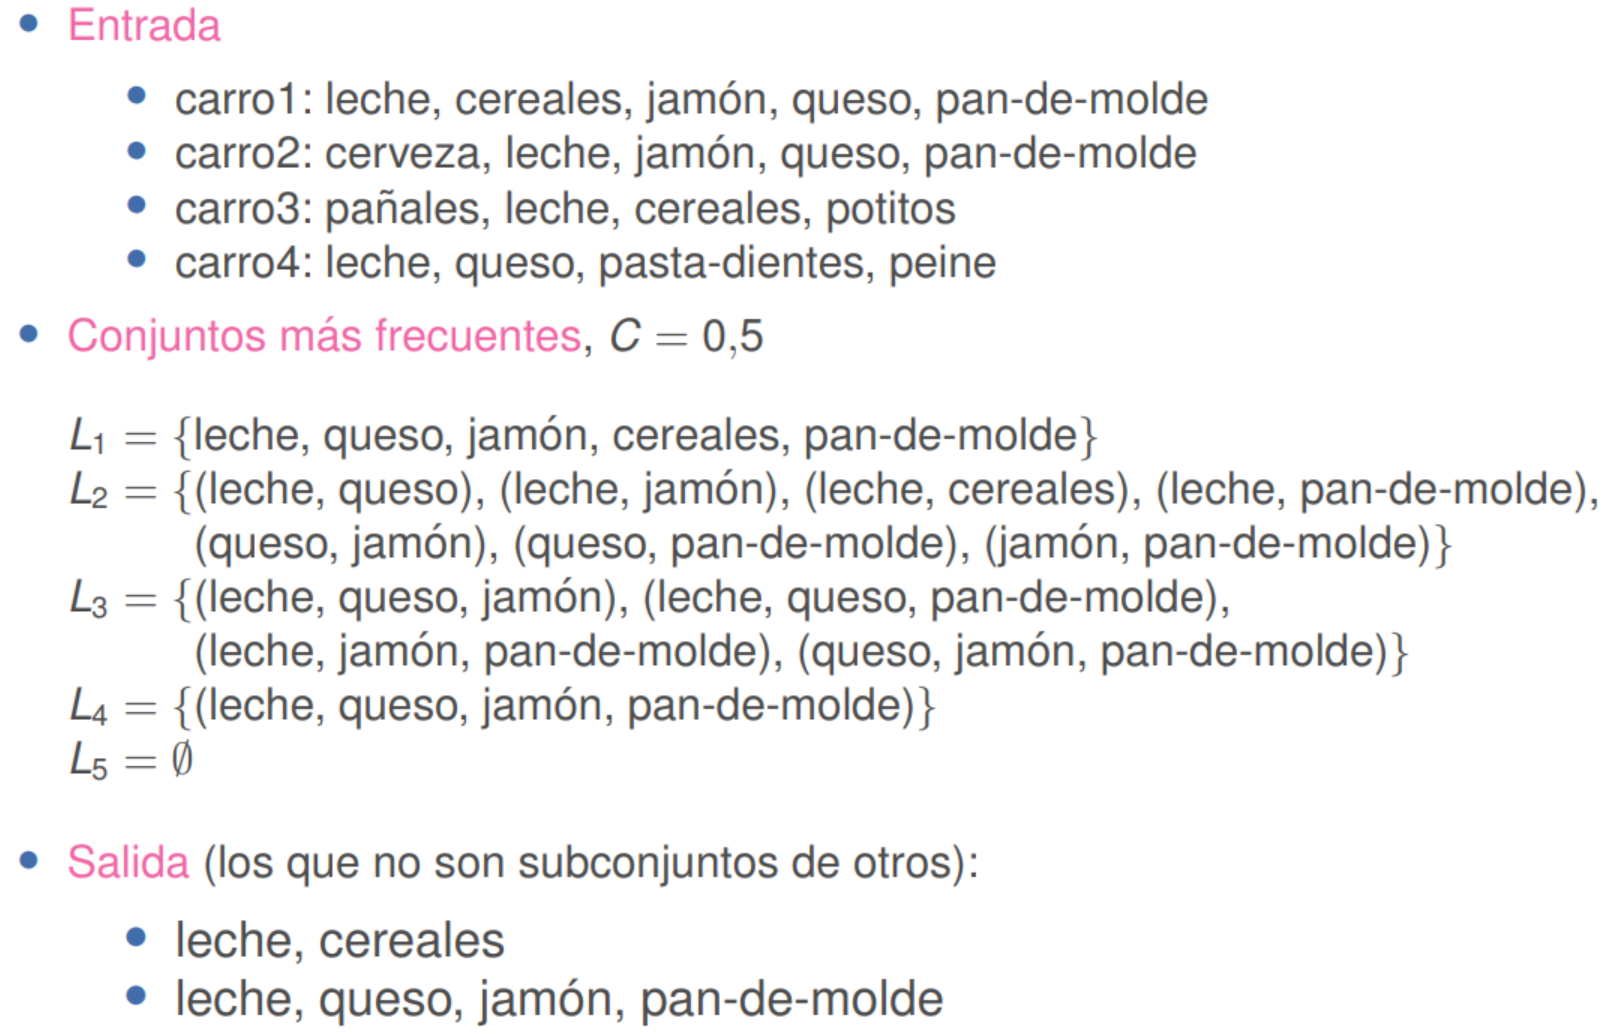
\includegraphics[scale=.4]{2021-04-10 01_06_33-ensembles-reglasAsociacion.pdf - Foxit Reader.png}}
\end{figure}

\subsection{Reglas de asociación}
\textbf{Objetivo:} Dados conjuntos de ejemplos, trata de determinar reglas que relacionen los elementos.

Se suelen utilizar como entrada los conjuntos más frecuentes.

Se calcula la precisión (confianza) de cada regla.

Se suelen escoger las que maximicen la precisión, las que sobrepasen un umbral de precisión y las N que tengan mayor precisión.

\begin{center}
  $X \Rightarrow Y$
\end{center}

\textbf{Soporte de la regla:} número de veces que el par antecedente-consecuente se dan juntos en los ejemplos.
$$C = \frac{|X, Y|}{|N|}$$

\textbf{Precisión (confianza) de la regla:} número de veces que el par antecedente-consecuente se dan juntos en los ejemplos sobre el número de veces que el antecedente es cierto.
$$P = \frac{|X, Y|}{|X|}$$

La idea es elegir las reglas cuya cobertura es mayor que un umbral de cobertura y cuya precisión sea mayor que un umbral de precisión.

\begin{figure}[H]
  \ffigbox[\FBwidth]
  {\caption{Ejemplo. Reglas de asociación I}}
  {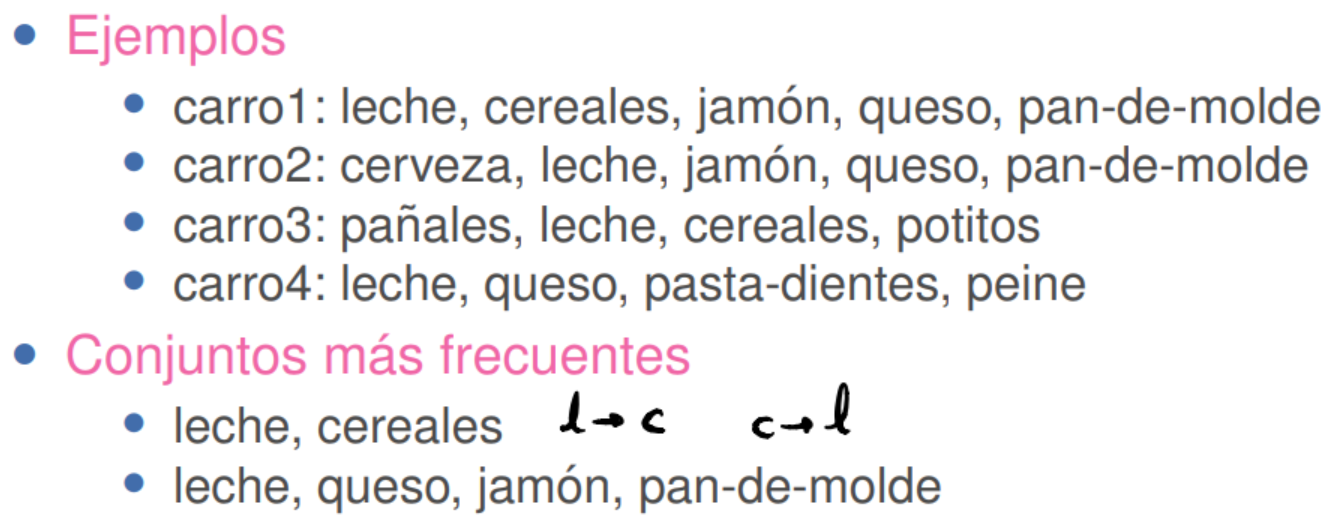
\includegraphics[scale=.3]{2021-04-10 01_17_45-ensembles-reglasAsociacion.pdf - Foxit Reader.png}}
\end{figure}

\begin{figure}[H]
  \ffigbox[\FBwidth]
  {\caption{Ejemplo. Reglas de asociación II}}
  {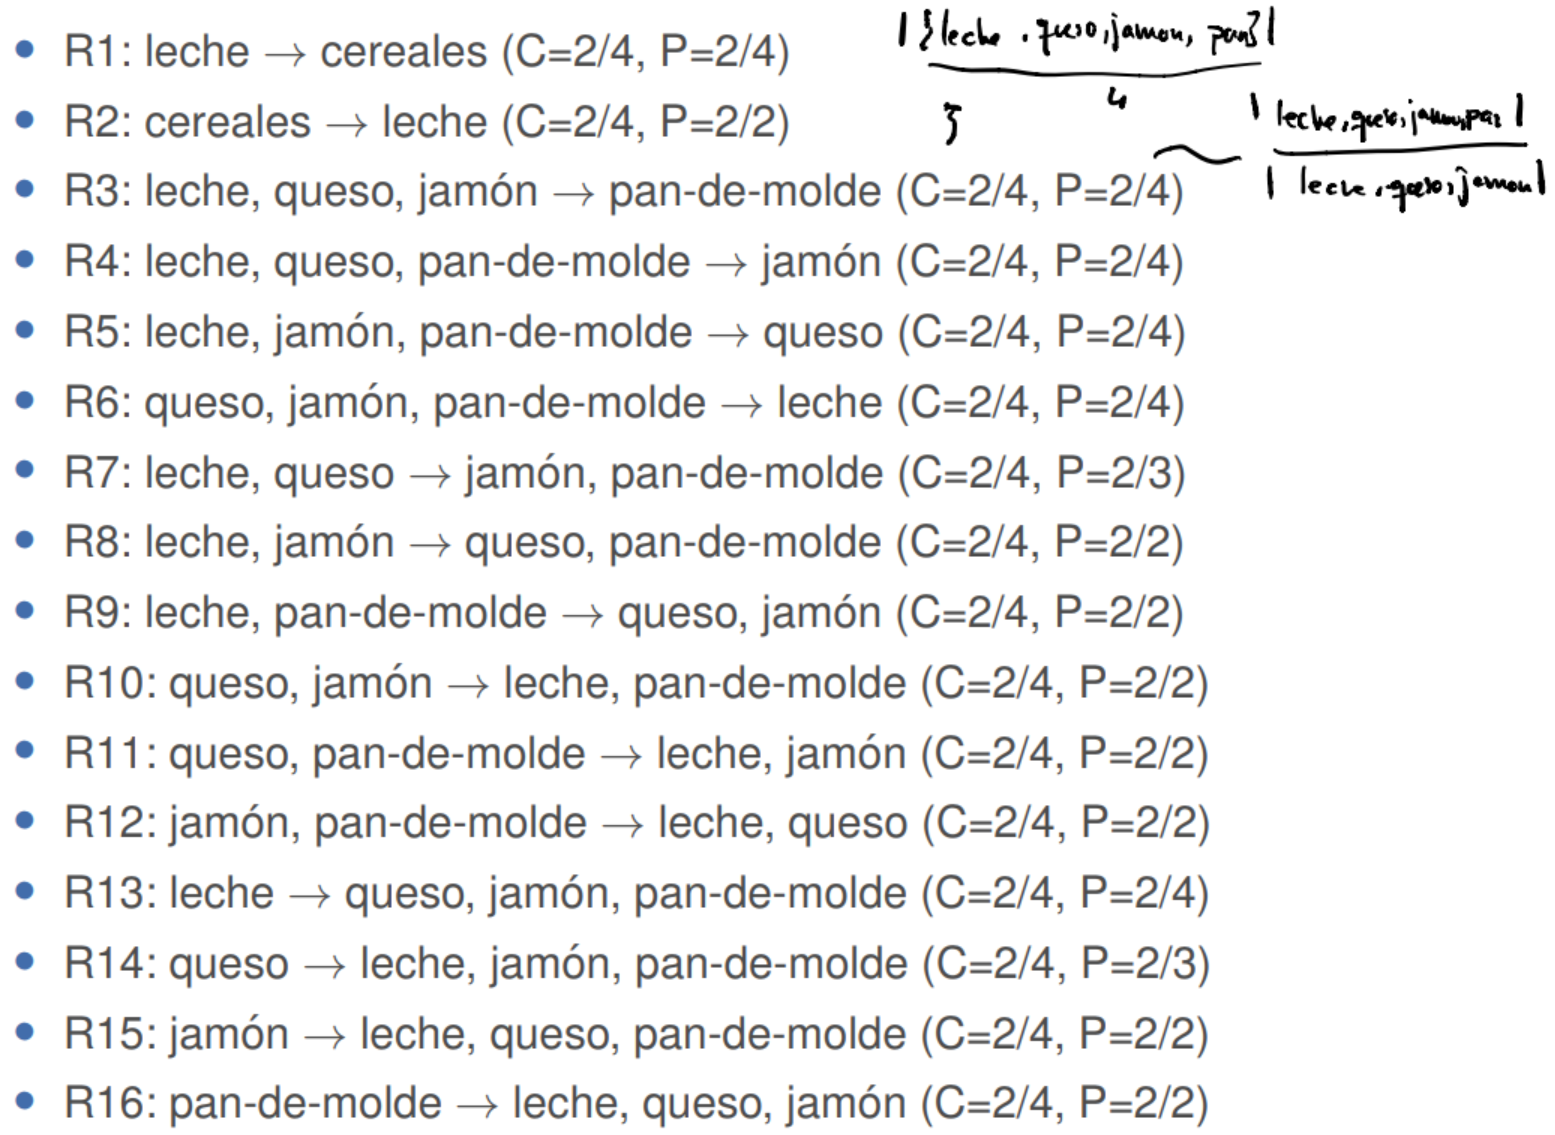
\includegraphics[scale=.3]{2021-04-10 01_18_02-ensembles-reglasAsociacion.pdf - Foxit Reader.png}}
\end{figure}

\textbf{Si se parte de ejemplos atributo-valor:} Se define un elemento por cada valor del atributo (Si salario puede ser alto o bajo, los elementos serán salarioAlto y salarioBajo), de tal manera que un ejemplo/instancia se define como el conjunto de los elementos de sus valores de atributos (sin que haya más de un elemento que se refiera al mismo atributo). Se ejecuta APRIORI: genera reglas de asociación.

\textbf{Ejemplo:}

\textbf{Si} numero-habitacionesAlto Y salarioMedio \textbf{Entonces} numero-hijosAlto

\textbf{Si} salarioAlto \textbf{Entonces} precio-viviendaAlto

\chapter{Tema 7: Aprendizaje por Refuerzo}
Consiste en aprender a decidir, ante una situación determinada, que acción es la más adecuada para lograr un objetivo.

Se utiliza una Política que acción, que dado un estado del agente nos diga cuál es la acción debe ejecutar, $\pi: s \rightarrow a$. 

Se construye a partir de experiencias de interacción con el entorno: $<s_i, a_i, s'_i, r_i>$ (estado actual, acción, estado siguiente, refuerzo)
\begin{figure}[H]
  \ffigbox[\FBwidth]
  {\caption{Diagrama Aprendizaje por refuerzo}}
  {\includegraphics[scale=.3]{default.jpg}}
\end{figure}

Mediante un proceso iterativo de prueba y error, en que se van proporcionando señales de refuerzo que premia (positivo) o castigan (negativo) las decisiones en el proceso de maximizar el refuerzo.

Por debajo del aprendizaje por refuerzo hay un Proceso de Decisión de Márkov.

\section{MDP - Markov Decision Process}

Se tiene una serie de estados en los que se pueden realizar unas determinadas acciones, aunque también se hay estados absorbentes en los que no se puede aplicar ninguna acción.

Las acciones \textbf{deterministas} siempre produce la misma transición de estado y el mismo refuerzo, sin embargo, en los \textbf{no deterministas/estocástico} un mismo estado y una acción pueden producir distintos resultados, son funciones estocásticas.

Se define con la tupla $<S, A, T, R>$:
\begin{itemize}
  \item S - Conjunto de Estados.
  \item A - Conjunto de Acciones.
  \item T - Función de Transición $T(s, a, s')$; dado un estado, una acción y el estado siguiente nos dice la probabilidad de que ocurra esa transición.
  \item R - Función de Refuerzo $R: S \times A \times S \rightarrow \mathbb{R}$, proporciona el refuerzo recibido al ejecutar la acción $a$ en estado $s$ y llegar al $s'$.
\end{itemize}

\subsection{Propiedad de Márkov}
Se asume que se cumple esta propiedad cuando realizamos un MDP.

\textbf{Propiedad de Márkov:} El pasado más allá del estado inmediatamente anterior no son relevantes, la acción a ejecutar solo depende del estado actual. El estado actual y el refuerzo obtenido son condicionalmente independientes de la historia pasada.
\begin{figure}[H]
  $$P(s_{t+1}, r_{t+1}| s_t,a_t)$$
    \captionsetup{justification=centering}
  \caption{Propiedad de Márkov}
\end{figure}

\subsection{Métodos de Resolución}
Hay dos posibilidades:
\begin{itemize}
  \item \textbf{Se conoce el modelo}, la Función de Transición de estados y la Función de Refuerzo del MDP.
  
  En este caso se utiliza \textbf{Programación Dinámica}, hay dos opciones.
  \begin{itemize}
    \item \textbf{Iteración de valor.}
    \item \textbf{Iteración de la política.}
  \end{itemize}

  \item \textbf{No se conoce el modelo}, hay dos opciones:
  \begin{itemize}
    \item \textbf{Aprender el modelo} y usar métodos basados en el modelo, Programación Dinámica.
    \item \textbf{Aprender las funciones de valor y/o políticas directamente}: métodos libres de modelo o Aprendizaje por Refuerzo.
  \end{itemize}
\end{itemize}

\subsection{Políticas y Optimalidad}

El \textbf{objetivo es encontrar una política}, $\pi: S \rightarrow A$, que nos diga para cada estado posible cuál es la acción que debe ejecutarse para maximizar el refuerzo acumulado en el tiempo.

\textbf{Criterio de optimalidad de horizonte infinito descontado}: Asumiendo que se suma hasta infinito, se valora más que se obtenga el mayor refuerzo lo antes posible, para esto se utiliza un factor de descuento, $0 \leq \gamma \leq 1$, que reduce la importancia de las ganancias futuras.
$$\sum ^\infty _{k=0} \gamma^k r_{t+1+k}$$

\pagebreak

\subsubsection{Función de Valor (V) - valor-estado}
Dada una política $\pi$ y un estado inicial s, $V^\pi (s)$ representa el refuerzo descontado en el tiempo si se aplica la política $\pi$ partiendo de s. En el caso no determinista es un valor esperado.

\begin{figure}[H]
  $$V^\pi(s_t)=E \left[ \sum ^\infty _{k=0} \gamma^k r_{t+1+k} \right]$$
  \captionsetup{justification=centering}
  \caption{Función de Valor}
\end{figure}

\subsubsection{Política óptima}
La política óptima $\pi^*$, es aquella que maximiza $V^\pi (s)$ para todos los estados. $V^* (s)$ es máximo refuerzo descontado acumulado en el tiempo que el agente puede conseguir comenzando en el estado s y siguiendo la política óptima $\pi^*$.

$$\pi ^* \equiv \arg \max_\pi V^\pi (s), \forall s \equiv V^* (s)$$


\subsubsection{Función de valor-acción (Q)}
Dada una política $\pi$, un estado inicial s y una acción a, $Q^\pi (s, a)$ representa el refuerzo descontado acumulado en el tiempo si se aplica la acción a en el estado s, y a partir de ahí se ejecuta la política $\pi$.

\begin{figure}[H]
  \begin{eqnarray*}
    Q^* (s, a) &=& \max_\pi Q^\pi (s,a), \forall s \in S, \forall a \in A \\
    V^* (s) &=& \max_a Q^* (s,a), \forall s \in S
  \end{eqnarray*} 
  \captionsetup{justification=centering}
  \caption{Función de valor-acción}
\end{figure}

Política optima en función de Q, maximiza el refuerzo de cada acción que se puede ejecutar en ese estado.
$$\pi^* (s) = \arg \max_{a \in A} Q^* (s,a), \forall s \in S$$
\pagebreak
\subsubsection{Ecuaciones de Bellman}
Ecuaciones recurrentes que se basan en calcular el refuerzo total óptimo maximizando sobre la elección de una primera acción y considerando un futuro óptimo.
\begin{figure}[H]
  \begin{eqnarray*}
    Q^* (s, a) &=& \sum _{s'} T(s,a, s') [R(s,a,s') + \gamma V^* (s')]\\
    V^* (s) &=& \max_a Q^*(s,a) = \max _a \sum _{s'} T(s,a, s') [R(s,a,s') + \gamma V^* (s')]
  \end{eqnarray*} 
  \captionsetup{justification=centering}
  \caption{Ecuaciones de Bellman}
\end{figure}

\subsection{Resolver el MDP: Aproximaciones Basadas en el Modelo}
La Función de Transición y la Función de Refuerzo son conocidas, se trata de resolver las ecuaciones de Bellman mediante Programación Dinámica y tenemos dos opciones que resuelven el mismo problema:
\subsubsection{Algoritmo Iteración de valor - Value Iteration}
\begin{itemize}
  \item Inicializar: $V(s) = 0$ para todo $s$
  \item Repetir hasta convergencia
  \begin{enumerate}
    \item Dados $V(s)$ para todo $s$, actualizar los valores para la nueva iteración teniendo en cuenta los de la anterior.
    $$V(s) = \max _a \sum _{s'} T(s,a, s') [R(s,a,s') + \gamma V^* (s')], \forall s$$
    \item La política generada en la iteración consiste en quedarnos con la acción que genera el mayor valor para cada estado posible. Aunque solo nos interesará en la última iteración que será la óptima.
    $$\pi(s) = \arg \max_a \sum _{s'} T(s,a, s') [R(s,a,s') + \gamma V^* (s')], \forall s$$
  \end{enumerate}
\end{itemize}
Cuando el algoritmo converge (los valores se estabilizan) la política es óptima.
\begin{figure}[H]
  \ffigbox[\FBwidth]
  {\caption{Algoritmo Iteración de valor}}
  {\includegraphics[scale=.3]{2021-04-16 13_01_42-refuerzo.pdf - Foxit Reader.png}}
\end{figure}

\subsubsection{Algoritmo Iteración de política - Policy Iteration}
Es como hacer Iteración valor, pero en la Ecuación de Bellman en vez de evaluar todas las acciones se evalúa solo la acción que proporciona la política que vamos actualizando, en cuanto al cálculo de la política es igual, por lo que debemos tener en cuenta todas las acciones en todos los estados (lo que parecía que nos ahorrábamos calcular, se calcula ahora).
\begin{itemize}
  \item Elegir una política $\pi$ arbitraria (aleatoria)
  \item Repetir hasta convergencia
  \begin{enumerate}
    \item Evaluación de la política: resolver las ecuaciones $\forall s \in S$
    $$V(s) = \sum _{s'} T(s,\pi(s), s') [R(s,\pi(s),s') + \gamma V^* (s')]$$
    \item Mejora de la política $\forall s \in S$
    $$\pi(s) = \arg \max_a \sum _{s'} T(s,a, s') [R(s,a,s') + \gamma V^* (s')], \forall s$$
  \end{enumerate}
\end{itemize}
Cuando el algoritmo converge (la política se estabiliza) la política es óptima.

\section{Aprendizaje por Refuerzo}
\subsection{Modelo desconocido}
Problema de Aprendizaje por Refuerzo (definido como un MDP):
\begin{itemize}
  \item Conjunto de todos los posibles estados, S.
  \item Conjunto de todas las posibles acciones, A.
  \item Función de Transición de estados desconocida $T: S\times A \times S \rightarrow \mathbb{R}$.
  \item Función de Refuerzo $R: S \times A \times S \rightarrow \mathbb{R}$.
\end{itemize}
\textbf{Objetivo:} aprender la política de acción,$\pi: S \rightarrow A$ , que maximice el refuerzo esperado acumulado en el tiempo mediante exploración del entorno.

\subsection{Aproximaciones Basadas en el Modelo}
\begin{enumerate}
  \item Se aprende el modelo (T y R) y se resuelven las ecuaciones por Programación Dinámica ( Iteración de valor o Política)
  \begin{itemize}
    \item Técnicas costosas computacionalmente.
    \item No útil para respuestas en tiempo real
    \item Se debe asegurar que se aprende el entorno completamente.
    \item No es sensible a cambios en el entorno 
  \end{itemize}
  \item Se aprende el modelo a la vez que la función Q (algoritmo Dyna-Q)
\end{enumerate}

\subsection{Aproximaciones libres de Modelo}
Aprende directamente del entorno mediante prueba y error.
\begin{itemize}
  \item Actualización directa de la función de valor Q a partir de interacciones con el entorno.
  \item Basados en procesos de prueba y error.
  \item NO aprenden el MDP subyacente.
\end{itemize}
Métodos Monte Carlo y métodos de Diferencia Temporal (Q-learning, SARSA)

\subsection{Métodos Monte Carlo (MC)}
El objetivo es estimar $Q^*$, el refuerzo que voy a obtener a futuro si aplico la opción óptima.

Basado en: 
\begin{itemize}
  \item Alternar la evaluación de política y su mejora, en sucesivas ejecuciones de episodios de aprendizaje.
  \item Actualización de Q basada en la media de los refuerzos en los episodios.
  \item Actualiza Q al final de cada episodio.
\end{itemize}

\subsubsection{Monte Carlo con Arranque Exploratorio}
\begin{itemize}
  \item Inicializar, $\forall s \in S, \forall a \in A$:
  \begin{itemize}
    \item $Q(s, a)$ valor arbitrario.
    \item $\pi(s)$ valor arbitrario.
    \item $ganancias(s, a)$ lista vacía.
  \end{itemize}
  \item Repetir para siempre:
  \begin{enumerate}
    \item Generar un episodio usando arranque exploratorio (comienza en un estado aleatorio) y la política $\pi$.
    \item Para cada par $(s, a)$ que aparece en el episodio:
    \begin{itemize}
      \item $R(s, a) = r + \gamma r'+ \gamma r''+ \gamma r'''+\dots$ refuerzo descontado acumulado tras (empezando a descontando con el refuerzo siguiente) la PRIMERA ocurrencia del par $(s, a)$. 
      \item Añadir $R(s, a)$ a $ganancias(s, a)$, cada par tiene su lista de refuerzos almacenados.
      \item $G = promedio(ganancias(s, a))$
      \item $Q(s, a) \leftarrow (1-\alpha)Q(s, a) + \alpha G$ (Caso determinista $\alpha = 1$, $Q(s, a) \leftarrow G$)
    \end{itemize}
    \item Para cada $s$ en el episodio: $\pi(s) \leftarrow \arg \max_a Q(s, a)$
  \end{enumerate}
\end{itemize}

\subsection{Métodos de Diferencia Temporal (TD)}
El objetivo es estimar $Q^*$.

Combinación de las ideas de Programación Dinámica y los métodos de Monte Carlo:
\begin{itemize}
  \item Aprendizaje por prueba y error. Estimaciones sobre estimaciones.
  \item Basado en el cálculo de las funciones de valor-acción Q.
  \item Se actualiza Q en el paso del episodio.
\end{itemize}

Algoritmos:
\begin{itemize}
  \item Q-Learning: off-policy (no lleva una política que vaya actualizando)
  \item SARSA (State–action–reward–state–action): on-policy
\end{itemize}

\subsubsection{Q-Learning}
Se basa en estimar de forma iterativa la función de valor-acción óptima, $Q^*(s, a)$. 

La función Q la podemos representar en forma de tabla con |S| filas y |A| columnas, en cada casilla se pondrá el refuerzo acumulado en el tiempo cuando en ese estado se ejecuta esa acción asumiendo refuerzo futuro óptimo.

Esta tabla que se genera nos facilita obtener la política óptima, de tal manera que la mejor acción de cada estado es el máximo de su fila.
$$\pi(s) = \arg \max _a Q^* (s, a)$$

Consiste en que después de cada transición se recalcula la tabla Q entera aproximándose poco a poco a la óptima, y se van generando episodios de aprendizaje, una serie de transiciones consecutivas hasta que termina o se para. $\underbrace{sas'} \underbrace{a'r's''} \underbrace{a''r''s'''}...$

\textbf{Funciones de Actualización de Q}
\begin{itemize}
  \item Función de Actualización \textbf{determinista}
  \begin{figure}[H]
    $$Q(s, a) \leftarrow r + \gamma \max_{a'} Q(s’, a')$$

    \captionsetup{justification=centering}
    \caption{Función de Actualización de Q Determinista}
  \end{figure}
  \item Función de actualización \textbf{no determinista} (en general)
  \begin{figure}[H]
    $$Q(s, a) \leftarrow (1-\alpha) Q(s, a) + \alpha[r + \gamma \max_{a'} Q(s’, a')]$$

    \captionsetup{justification=centering}
    \caption{Función de Actualización de Q No Determinista}
  \end{figure}
\end{itemize}

$\alpha \in [0,1]$ representa la tasa de aprendizaje, la agresividad con la que se actualiza la tabla.

$\gamma$ es el factor de descuento, como van perdiendo importancia las decisiones más alejadas del estado actual del agente.

\textbf{Algoritmo de Q-Learning($\gamma, \alpha$)}
En el que se realizan varios escenarios para ir mejorando la tabla Q, en cada uno de los escenarios se va evaluando la mejor acción para generar un estado completo (s, a, r, s') y se actualiza la tabla antes de transitar a él.
\begin{itemize}
  \item Inicializar $Q(s, a), \forall s \in S, a \in A$ (lo habitual es inicializar a 0)
  \item Repetir (para cada episodio)
  \begin{itemize}
    \item Inicializa el estado inicial, s, aleatoriamente.
    \item Repetir (para cada paso del episodio)
    \begin{itemize}
      \item Selecciona una acción a y la ejecuta.
      \item Recibe el estado actual s', y el refuerzo, r.
      \item $Q(s, a) \leftarrow (1-\alpha) Q(s, a) + \alpha[r + \gamma \max_{a'} Q(s’, a')]$      
      \item Asigna $s \leftarrow s'$
    \end{itemize}
  \end{itemize}
  \item Devuelve $Q(s, a)$.
\end{itemize}

\textbf{Ejemplo Q-Learning}

\begin{figure}[H]
  \ffigbox[\FBwidth]
  {\caption{Ejemplo Q-Learning I}}
  {\includegraphics[scale=.2]{2021-04-16 13_05_26-refuerzo.pdf - Foxit Reader.png}
  \includegraphics[scale=.25]{2021-04-16 13_05_47-refuerzo.pdf - Foxit Reader.png}}
\end{figure}
\begin{figure}[H]
  \ffigbox[\FBwidth]
  {\caption{Ejemplo Q-Learning II}}
  {\includegraphics[scale=.2]{2021-04-16 13_07_03-refuerzo.pdf - Foxit Reader.png}
  \includegraphics[scale=.2]{2021-04-16 13_07_51-refuerzo.pdf - Foxit Reader.png}}
\end{figure}

\subsection{Exploración vs. Explotación}

\textbf{Exploración:} Acciones aleatorias.

\textbf{Explotación:} Utilizar acciones de la política actual $\pi (s)=\arg \max _a Q (s, a)$

\textbf{Estrategias principales de selección de acciones}, para balancear la exploración y la explotación sesgando la selección de acciones con conocimiento del dominio:
\begin{itemize}
  \item \textbf{$\epsilon-greedy$:} Ejecuta una acción aleatoria con probabilidad $\epsilon$ y la acción $\arg \max_a Q(s, a)$ con probabilidad $1-\epsilon$
  \item \textbf{Softmax:} A cada acción que se puede ejecutar en un estado se le asigna una probabilidad.
  $$ P(a_i|s)= \frac{e^{Q(s, a_i)/\tau}} {\Sigma_{a_j \in A} e^{Q(s, a_j)/\tau}} $$
  
  Se utiliza un parámetro llamado Temperatura $\tau$, si es alta la acción es equiprobable (exploración pura), si es media es más probabilidad la que tiene mayor $Q(s, a)$ y si es baja se sigue la política (exploración pura).

  Lo ideal es que de más probabilidad a aquellas con mayor $Q(s, a)$, de tal manera que es aleatorio, pero la mejor acción es más probable.
\end{itemize}

\subsection{Aplicaciones}
Tiene muchas aplicaciones entre las que destaca la planificación en tiempo real y para entornos estocásticos.
\begin{itemize}
  \item Control de dispositivos de salud.
  \item Control de robots.
  \item Control de procesos de fabricación.
  \item Control de temperatura.
  \item Predicción de series.
  \item Juegos: AlphaGo, TD-Gammon.
  \item Logística.
  \item Problemas canónicos: navegación en un grid, balance de un sistema cart-pole.
\end{itemize}

\section{Representación de la función Q}
\subsection{Pac-Man}
\textbf{Observaciones:} coordenadas discretas x e y de Pac-Man y fantasmas.

\textbf{Acciones:} movimientos de tamaño 1 en las 4 direcciones.

\textbf{Objetivo:} comer fantasmas.

\subsection{Representación Tabular de la Función Q}
\textbf{Problema:} espacio de estados continuo o de gran tamaño.

\textbf{Solución:} métodos de generalización, abstracción: 
\begin{itemize}
  \item \textbf{Aproximaciones ad-hoc} basadas en conocimiento del dominio.
  \item \textbf{Discretización} del espacio de estados, pasar de continuo a discreto.
  \item \textbf{Aproximación de funciones}, en vez de una tabla discreta que sea una función.
\end{itemize}

\subsection{Mountain-Cart}
\textbf{Observaciones:} valores continuos de posición $x$ y velocidad $v$ del coche.

\textbf{Acciones:} aplicación de fuerza hacia la derecha, izquierda, o nula.

\textbf{Objetivo:} alcanzar la bandera con velocidad 0.

\section{Generalización en Aprendizaje por Refuerzo}
\subsection{Discretización del Espacio de Estados}
Los problemas que surgen al discretizar son:
\begin{itemize}
  \item Las discretizaciones erróneas pueden romper fácilmente la propiedad de Márkov.
  
  Al discretizar puede dejar de ser determinista, ya que puede ocurrir que al hacer una acción no se salga siempre del estado (como ocurriría en Pac-man si en vez de ir casilla a casilla son de 2x2).

  \item El número de regiones necesarias para discretizar el espacio de estados.
\end{itemize}

\subsection{Discretización uniforme del espacio de estados}
Discretizar cada atributo en un número dado de niveles de discretización o regiones, todas las regiones del mismo tamaño.

Esto supone un problema porque no se tiene en cuenta el número de ejemplos por región, por lo que puede haber regiones que no tengan ninguno y otras que estén superpobladas.

Se debería especializar más en las que tienen más ejemplos.

\subsection{Discretización de Resolución Variable: Árboles KD}
La discretización más fina en las regiones que más ejemplos hay.

Los nodos y hojas del árbol representan regiones del espacio de estados.

En cada nodo del árbol, una región se divide en otras dos, esta división se realizará según un criterio.

Con esta técnica una región se irá partiendo en dos hasta que cumpla las condiciones establecidas, y se crearan regiones más grandes para las menos pobladas y más pequeñas para las superpobladas.

\begin{figure}[H]
  \ffigbox[\FBwidth]
  {\caption{Discretización: Árbol KD}}
  {\includegraphics[scale=.25]{2021-04-24 14_09_21-refuerzo.pdf - Foxit Reader.png}}
\end{figure}

\subsection{Clustering (Agrupamiento) para Q-Learning}
\begin{enumerate}
  \item Discretización no uniforme del espacio de estados (k-means).
  \item Los clústeres obtenidos se consideran la nueva representación del espacio de estados.
  
  $sars' \rightarrow C_5arC_7$
  \item Se aplica Q-Learning sobre la nueva representación.
\end{enumerate}

\chapter{Tema 8: Programación Lógica Inductiva - ILP}
Aprendizaje para cuando tenemos los datos expresados de manera relacional.

Se hace cuando el conocimiento no se puede representar como atributo-valor o tengan relación entre los datos difíciles de expresar.

Método que emplearemos: FOIL - First Order Inductive Learner (Quinlan 1990).

Es aprendizaje supervisado, inductivo, generaliza con los ejemplos.

\section{Aprendizaje Relacional}
TILDE - Árboles de decisión.

WARMR - Reglas de Asociación, conjuntos frecuentes.

\section{Proposicionalización}
Lo que se puede hacer con la información relacional es pasarla a proposicional, hace mediante:
\begin{itemize}
  \item \textbf{Agregación}: Sumar los valores de distintos atributos para juntarlos en un atributo, el problema es que se pierde información.
  \item \textbf{Introducir atributos nuevos} en la tabla original, tantos como registros haya. El problema es que muchos atributos tendrán valores desconocidos.
\end{itemize}

\section{Elementos de representación}
\begin{itemize}
  \item \textbf{Términos}: Cualquier secuencia que empieza en minúsculas es una constante y en mayúsculas es una variable. También funciones que tiene como parámetros constantes y variables. $a$, $X$ y $fun(X,Y)$
  \item \textbf{Fórmulas atómicas}: Predicados definidos sobre términos. $tipo-cliente(X, bueno)$
  \item \textbf{Literal}: Fórmula atómica o su negación ($\neg$).
  \item \textbf{Clausula}: Disyunción de literales, oes de literales. $cliente(X,Y)\vee cliente(X,Z)$
  \item \textbf{Fórmulas bien formadas}: Fórmulas atómicas unidas por conectivas ($\wedge, \vee, \rightarrow, \neg$) y cuantificadas ($\forall, \exists$)
  \item \textbf{Clausula de Horn:} Clausula, disyunción de literales, que como mucho tiene un literal positivo. $\neg p \vee \neg q \vee \neg r \vee s$ que es $p \wedge q \wedge r \rightarrow s$ ($cuerpo \rightarrow cabeza$ que en prolog es $consecuente:-antecedente$).
  \item \textbf{Regla de Horn:} Conjunto de cláusulas de Horn. Si se da una de las cláusulas se cumple la regla.
  \item \textbf{Definición implícita:} Definido como una regla de Horn, de manera genérica.
  \item \textbf{Definición explicita:} Definido como todos los argumentos válidos que hace que se cumplan.
\end{itemize}

\section{Generalización simple. Subsunción}
Dada una sustitución $\theta= \{v_1/t_1, . . . , v_n/t_n\}$ y una fórmula $F$, $F\theta$ es el resultado de aplicar la sustitución sobre F.

Que una sentencia sea más general que otra quiere decir que conociendo la general se puede deducir el otro.

\textbf{Átomo A subsume al átomo B}, $A \succeq B$, si al aplicar la sustitución sobre A es igual a B.

\textbf{Cláusula C subsume a la cláusula D}, $C \succeq D$, si al aplicar la sustitución sobre C está contenida en D.

\section{Generalización como consecuencia lógica}
\textbf{Consecuencia lógica:} La consecuencia lógica se indica con $C \vDash D$, indica que conocido el antecedente se puede deducir el consecuente.

\textbf{Consecuencia lógica relativa:} La consecuencia lógica se indica con $B,C \vDash D$, indica que conocido el antecedente y un conocimiento base se puede deducir el consecuente.

\section{ILP - Programación Inductiva Lógica}
Lo que buscamos es generar una hipótesis de manera que junto al conocimiento base, los ejemplos sean una consecuencia lógica relativa.
$$B,H \vDash E$$
\begin{itemize}
  \item \textbf{B}: Conocimiento base.
  \item \textbf{E}: Conjunto de Ejemplos.
  \item \textbf{H}: Hipótesis.
\end{itemize}

Se trata de una búsqueda en el espacio de cláusulas que se llama \textbf{Refinamiento de Cláusulas}, los algoritmos que se emplean son:
\begin{itemize}
  \item Más específico a más general, como GOLEM.
  \item Más general a más específico, como FOIL o PROLOG.
\end{itemize} 

\section{FOIL - First Order Inductive Learner}
Aprendizaje inductivo de reglas de Horn, de más general a más específico, mediante una búsqueda en escalada con heurística en el espacio de cláusulas.

\subsection{Algoritmo de FOIL}
\textbf{Función FOIL (E+, E-, P, B): REGLA}

$E^+$ y $E^-$ ejemplos positivos y negativos del concepto meta resp., P predicado a aprender, B conocimiento de base.
\begin{itemize}
  \item Hasta que $E^+ = \emptyset$, es decir que están cubiertos por alguna cláusula:
  \begin{itemize}
    \item $N = E^-$
    \item Clausula limpia, $CUERPO = \emptyset$
    \item Hasta que $N = \emptyset$, que no deje pasar ejemplos negativos
    \begin{itemize}
      \item $L = literal-maxima-ganancia(E^+, E^-, P, B, N, CUERPO)$
      \item Se añade un literal al cuerpo, $CUERPO = CUERPO, L$
      \item Se quitan de N los ejemplos negativos que no deja pasar el literal, $N = N - \{e \in N | L \nvDash e\}$
    \end{itemize}  
    \item Se añade la cláusula a las reglas, $REGLA = REGLA \cup [P:-CUERPO]$
    \item Se quitan los ejemplos positivos cubiertos por la regla, $E^+ = E^+ - \{e \in E^+ | CUERPO \vDash e\}$
  \end{itemize}
  \item Devolver $REGLA$
\end{itemize}
\pagebreak
\subsection{Heurística de FOIL}
$$G(L)=k\times [I(n^+,n^-)-I(n^+_L, n^-_L)]$$
\begin{itemize}
  \item $G(L)$: Ganancia que se obtiene al añadir el literal L a la cláusula.
  \item $k$: Número de ejemplos positivos que se cumplen con el conocimiento base B con L.
  \item $n^+$: Número de tuplas de la cláusula que hacen ciertos ejemplos positivos.
  \item $n^-$: Número de tuplas de la cláusula que hacen ciertos ejemplos negativos.
  \item $n^+_L$: Número de tuplas de la cláusula con el L que hacen ciertos ejemplos positivos.
  \item $n^-_L$: Número de tuplas de la cláusula con el L que hacen ciertos ejemplos negativos.
  \item $I(x, y)=-\log_2 \left( \frac{x}{x-y} \right)$ la x son las positivas y la y la negativa.
\end{itemize}

\subsection{Tipos de literales}
\begin{itemize}
  \item Literales: $Q(V_1, V_2, ..., V_n)$, $\neg Q(V_1, V_2, ..., V_n)$.
  \item Desigualdades: $X_i < c, X_i < X_j, X_i > c, X_i > X_j, X_i <= c, X_i <= X_j, X_i >= c, X_i >= X_j$.
  \item Igualdades: $X_i = c, X_i = X_j, X_i \neq c, X_i \neq X_j$.
\end{itemize}
Los literales deben proceder de B.

En los literales se pueden utilizar variables nuevas.

En las comparaciones o desigualdades se usan variables que aparecen previamente.

\subsection{Otras restricciones}
\begin{itemize}
  \item Q debe tener al menos una variable ya existente
  \item No permite funciones ni constantes en las reglas aprendidas.
  \item El conocimiento debe estar definido extensionalmente, que es costoso.
  \item Se puede hacer poda cuando la ganancia este por debajo de un umbral.
  \item FOIL permite obtener definiciones recursivas.
\end{itemize}

\subsection{Sesgo o bias}
El espacio de búsqueda es mucho mayor que con representación atributo-valor, por lo que es necesario restringir:
\begin{itemize}
  \item El lenguaje en las cláusulas, no permitiendo funciones, ni contantes o solo atributos nuevos en los literales (al menos uno conocido).
  \item Profundidad de recursión o número de variables.
  \item Predicados procedentes del conocimiento base.
  \item Heurísticas: definida por la función de ganancia.
  \item Modos de los predicados.
\end{itemize}

\subsection{Otros algoritmos relacionales}
\begin{itemize}
  \item Reglas de decisión relacionales: PROGOL, GOLEM
  \item Árboles de decisión relacionales: TILDE
  \item Árboles de regresión relacionales: S-CART, TILDE-RT
  \item Basado en instancias relacionales: RIBL
  \item Aprendizaje modelos probabilísticos relacionales
  \item Por refuerzo relacional: RRL
  \item Clustering relacional: FORC=K-MEDIAS relacional
  \item Reglas de asociación o conjuntos frecuentes relacionales: APRIORI, WARMR
  \item Aprendizaje de atributos relevantes con ILP: LINUS
  \item Híbridos: árboles de decisión con IBL en los nodos hoja
\end{itemize}

\chapter{Resumen}
\section{Selección}
\textbf{Clase etiqueta:} Árboles y reglas de decisión, KNN, Ensembles, Naïve Bayes, FOIL.

\textbf{Probabilidad de las clases o text mining:} Naïve Bayes.

\textbf{Muchos datos y difícil atributo-valor:} Relacional.

\textbf{Clase numérica:} M5, CART, Ensembles o KNN.

\textbf{Agrupar elementos:} k-medias.

\textbf{Agrupar jerárquicamente o grupos:} Aglomerativos.

\textbf{Asociaciones o elementos por su frecuencia:} APRIORI y Reglas de asociación.

\textbf{Tomar decisiones, transiciones y recompensa:} Q-learning, Monte Carlo o Dyna-Q

\textbf{Tomar decisiones, pero (S, A, T, R) conocido:} Programación dinámica.

\section{Aprendizaje supervisado}
Si va a haber atributos con valores vacíos usar representación relacional.
\begin{itemize}
  \item \textbf{Árboles de reglas de decisión:} Definir el nivel de poda, limpieza de los atributos y la selección de los atributos
  \begin{itemize}
    \item \textbf{ID3:} No con atributos numéricos o discretos con muchos valores.
    \item \textbf{C4.5 y J48:} Con atributos numéricos o cuando se tengan muchos.
  \end{itemize}
  \item \textbf{Aprendizaje basado en instancias (IBK):} KNN.
  \begin{itemize}
    \item Definir el valor de k y la medida de similitud.
    \item Limpiar los atributos con wrapper, normalizar o ponderar (si no se normaliza)
    \item Limpiar el conjunto de ejemplos, borrando o con centroides.
  \end{itemize}
  \item \textbf{Naïve Bayes (text mining):} Clasificación probabilística.
  \begin{itemize}
    \item No hay parámetros que configurar, es calcular las tablas.
    \item Permite trabajar con valores continuos (no hace falta discretizar)
  \end{itemize}
  \item \textbf{Deep Learning (imágenes y sonido):} Trabaja con los datos en bruto.
  \item \textbf{Relacional: FOIL}, es aprendizaje relacional y hay que definir Conocimiento base, el predicado a aprender y los ejemplos que se usaran para entrenar.
\end{itemize}
\textbf{Tipos:}
\begin{itemize}
  \item \textbf{Clasificación}
  \begin{itemize}
    \item Árboles y reglas de Decisión: ID3, C4.5, J48
    \item Aprendizaje basado en instancias: KNN
    \item Conjuntos de clasificadores
    \item Naïve Bayes y Clasificador Bayesiano
    \item Relacional: FOIL
  \end{itemize}
  \item \textbf{Regresión}
  \begin{itemize}
    \item Aprendizaje basado en instancias: KNN
    \item CART y M5
    \item Conjuntos de clasificadores
    \item Naïve Bayes, Redes neuronales, Deep Learning
  \end{itemize}
  \item \textbf{En relacional mirar la lista}, tiene posibles para todos
\end{itemize}

\section{Aprendizaje no supervisado}
\begin{itemize}
  \item \textbf{Clustering:} k-medias
  \begin{itemize}
    \item Definir el valor de k, medida de distancia, semillas y normalización/ponderar.
  \end{itemize}
  \item \textbf{Aglomerativos:} Clustering jerárquico, que genera un dendrograma.
  \begin{itemize}
    \item Definir medida de distancia, como tratar jerarquía y normalización/ponderar.
  \end{itemize}
  \item \textbf{Reglas de asociación y Conjuntos frecuentes:} APRIORI, aprendizaje asociativo
  \begin{itemize}
    \item Definir la cobertura.
    \item Si hay valores numéricos continuos discretizar.
    \item Explicar: primero conjuntos frecuentes y genera las reglas.
    \item Definir como será las reglas objetiva.
    \item Si se quiere tener en cuenta el orden, se busca no solo que aparezcan sino también el orden. Cuando aumenta el tamaño del conjunto salen más combinaciones.
  \end{itemize}
\end{itemize}

\section{Aprendizaje por refuerzo}
Definir Estados, Acciones, función de Transición (si es conocida) y función de Refuerzo (retardada casi siempre, los inmediatos llevan a comportamientos cortoplacistas)

\begin{itemize}
  \item \textbf{Q-learning}
  \begin{itemize}
    \item Indicar el factor de reducción $\gamma$ y de aprendizaje $\alpha$ si no es determinista.
    \item Determinar que exploración/explotación usaremos: $\epsilon$-greedy o Softmax
    \item Si la situación para la que se crea es crítica, entrenarlo en un simulador realista.
  \end{itemize}
  \item \textbf{Basada en el modelo: Dyna-Q}, no es buena para tiempo real.
\end{itemize}

\textbf{Factores que apuntan a este aprendizaje:}
\begin{itemize}
  \item Tarea de toma de decisiones secuenciales.
  \item Se puede entender un MDP subyacente.
  \item No se conoce a priori cuál es la mejor acción en cada situación.
  \item Que sea de prueba y error.
  \item El beneficio/impacto solo se conoce al final del episodio.
\end{itemize}

\section{Normalizar valores numericos}
$$z_i = \frac{x_i - \min x}{\max x - \min x}$$

\section{Tratamiento de valores nominales en distancias}
\begin{itemize}
  \item \textbf{Binarios:} Asignar a cada opción uno de los valores y hacer Hamming, 1 o 0.
  \item \textbf{Ordinarios:} Primaria, ESO o Bachillerato. Asignar números según el orden y usarlos normal; 0, 1 y 3.
  \item \textbf{Categóricos:} Rojo, Verde o Azul. Asignar números arbitrarios y usarlos normal; 1, 2 y 3.
\end{itemize}
\textbf{Distancia Hamming:} En vez de poner $(x_i - x_j)^2$ en la distancia euclídea se pone 0 o 1.
\begin{itemize}
  \item 0 si $x_i = x_j$
  \item 1 si $x_i \neq x_j$
\end{itemize}

\end{document}
